\section{Fields and Galois Theory}
The first principal theme of this chapter is the structure theory of fields. We shall 
study a field $F$ in terms of a specified subfield $K$ ($F$ is said to be an extension field of $K$). The basic facts about field extensions are developed, in particular, the distinction between algebraic and transcendental extensions. For the most part we deal only with algebraic extensions in this section. Arbitrary field extensions are considered in the next chapter. The structure of certain fields and field extensions is thoroughly analyzed: simple extensions; splitting fields (normal extensions) and algebraic closures; finite fields; and separable algebraic extensions. 
The Galois theory of field extensions (the other main theme of this chapter) had its historical origin in a classical problem in the theory of equations. Various results of Galois theory have important applications, especially in the study of algebraic numbers and algebraic geometry.
\subsection{Field Extensions}
The basic facts needed for the study of field extensions are presented first, followed by a discussion of simple extensions. Finally a number of essential properties of algebraic extensions are proved. In the appendix, several famous geometric problems of antiquity are settled, such as the trisection of an angle by ruler and compass constructions.
\begin{definition}
A field $F$ is said to be an \textbf{extension field} of $K$ (or simply an extension of $K$) provided that $K$ is a subfield of $F$.
\end{definition}
If $F$ is an extension field of $K$, then it is easy to see that $1_K=1_F$. Furthermore, $F$ is a vector space over $K$. Throughout this chapter the dimension of $K$-vector space $F$ will be denoted $[F:K]$. $F$ is said to be a \textbf{finite dimension extension} or \textbf{infinite dimensional extension} of $K$ according as $[F:K]$ is finite or infinite. By Theorem 5.25 we have $[F:K]=[F:E][E:K]$ if $F$ is an extension of $E$, and $E$ is an extension of $K$. Furthermore $[F:K]$ is finite if and only if $[F:E]$ and $[E:K]$ are both finite.\par
In the situation $F\supset E\supset K$, $E$ is said to be an \textbf{intermediate field} of $K$ and $F$. If $F$ is a field and $X\subset F$, then the \textbf{subfield} [resp. \textbf{subring}] \textbf{generated by $X$} is the intersection of all subfields [resp. subrings] of $F$ of $F$ that contain $X$. If $f$ is an extension of $K$ and $X\subset F$, then the subfield [resp. subring] generated by $K\cup X$ is called the \textbf{subfield} [resp. \textbf{subring}] \textbf{generated by $X$ over $K$} and is denoted $K(X)$ [resp. $K[X]$]. Note that $K[X]$ is necessarily an integral domain.\par
If $X=\{u_1,\cdots,u_n\}$, then the subfield $K(X)$ [resp. subring $K[X]$] of $F$ is denoted $K(u_1,\cdots,u_n)$ [resp. $K[u_1,\cdots,u_n]$]. The field $K(u_1,\cdots,u_n)$ is said to be \textbf{finitely generated extension} of $K$. If $X=\{u\}$, then $K(u)$ is said to be a \textbf{simple extension} of $K$. A routine verification shows that neither $K(u_1,\cdots,u_n)$ nor $K[u_1,\cdots,u_n]$ depends on the order of the $u_i$ and 
$$
K\left( u_1,\cdots ,u_{n-1} \right) \left( u_n \right) =K\left( u_1,\cdots ,u_n \right) ,\hspace{0.5cm}K\left[ u_1,\cdots ,u_{n-1} \right] \left[ u_n \right] =K\left[ u_1,\cdots ,u_n \right] .
$$
If $F$ is a field and $u,v\in F$, we shall write $uv^{-1}=u/v$ under some circumstances.\par
We now introduce some basic properties of the field $K(X)$ and the ring $K[X]$.
\begin{theorem}
If $F$ is an extension field of a field $K$, $u,u_i\in F$ and $X\subset F$, then \par
(i) The subring $K[u]$ [resp. $K[u_1,\cdots,u_m]$; $K[X]$] consists of all elements of the form $f(u)$ [resp. $g(u_1,\cdots,u_m)$; $h(u_1,\cdots,u_n)$], where $f$ is a polynomial with coefficients in $K$ [resp. $g$ is a polynomial in $m$ indeterminates with coefficients in $K$; each $u_i\in X$ and $h$ is a polynomial in $n$ indeterminates with coefficients in $K$].\par
(ii) The subfield $K(u)$ [resp. $K(u_1,\cdots,u_m)$; $K(X)$] consists of all elements of the form $f(u)/g(u)$ [resp. $h(u_1,\cdots,u_m)/k(u_1,\cdots,u_m)$; $f(u_1,\cdots,u_n)/g(u_1,\cdots,u_n)$], where $f$ and $g$ are polynomials with coefficients in $K$ and $g(u)\ne 0$ [resp. $h$ and $k$ are polynomials in $m$ indeterminates with coefficients in $K$ and $k(u_1,\cdots,u_m)\ne 0$; each $u_i\in X$, and $f$ and $g$ are polynomials in $n$ indeterminates with coefficients in $K$ and $g(u_1,\cdots,u_n)\ne 0$].\par
(iii) For each $v\in K(X)$ [resp. $K[X]$], there is a finite subset $X^\prime$ of $X$ such that $v\in K(X^\prime)$ [resp. $v\in K[X^\prime]$].
\end{theorem}
\begin{proof}
We only prove the most generalized situation, and the others follows immediately.\par
(i) Let $E$ be the set of all $h(x_1,\cdots,x_n)$, where $n\in\mathbb{N}$, $x_i\in X$ and $h$ a polynomial with $n$ intermediates. By definition of $K[X]$ we have $K[X]\supset E$. Now we show the converse inclusion, which suffices to show that $E$ is a ring. Suppose $h_1(x_1,\cdots,x_m)$ and $h_2(x_{m+1},\cdots,x_n)\in E$, then clearly $h(x_1,\cdots,x_n)=h_1(x_1,\cdots,x_m)+h_2(x_{m+1},\cdots,x_n)\in E$, therefore $E$ is an additive group. Similarly we have $E$ a ring, and hence $K[X]\subset E$. Therefore $K[X]=E$.\par
(ii) Let $E$ be the set of all $f(u_1,\cdots,u_n)/g(u_1,\cdots,u_n)$, where $n\in\mathbb{N}$, $u_i\in X$ and $f,g$ polynomials with $n$ intermediates, and $g9u-1,\cdots,u_n)\ne 0$. Clearly $K(X)\supset E$. For the converse inclusion, suppose $f(u_1,\cdots,u_m)/g(u_1,\cdots,u_m)$ and $f_1(u_{m+1},\cdots,u_n)/g_1(u_{m+1},\cdots,u_n)\in E$. Define 
$$
h\left( x_1,\cdots ,x_n \right) =f\left( x_1,\cdots ,x_m \right) g_1\left( x_{m+1},\cdots ,x_n \right) -f_1\left( x_{m+1},\cdots ,x_n \right) g\left( x_1,\cdots ,x_m \right) 
$$
and 
$$
k\left( x_1,\cdots ,x_n \right) =g\left( x_1,\cdots ,x_m \right) g_1\left( x_{m+1},\cdots ,x_n \right) ,
$$
then 
$$
\frac{f\left( u_1,\cdots ,u_m \right)}{g\left( u_1,\cdots ,u_m \right)}-\frac{f_1\left( u_{m+1},\cdots u_n \right)}{g_1\left( u_{m+1},\cdots ,u_n \right)}=\frac{h\left( u_1,\cdots ,u_n \right)}{k\left( u_1,\cdots ,u_n \right)}\in E.
$$
Therefore $E$ is an additive group. Similarly one may show that the nonzero elements of $E$ form a group under multiplication, whence $E$ is a field. Since $K\subset E$ and $X\subset E$, we have $K(X)\subset E$, hence $K(X)=E$.\par
(iii) By (ii), suppose $u\in K(X)$, then $u=h(u_1,\cdots,u_n)/k(u_1,\cdots,u_n)$. Therefore let $X^\prime=\{u_1,\cdots,u_n\}\subset X$.
\end{proof}
If $L$ and $M$ are subfields of a field $F$, the \textbf{composite} of $L$ and $M$ in $F$, denoted $LM$ is the subfield generated by the set $L\cup M$. An immediate consequence of this definition is that $LM=L(M)=M(L)$. It is easy to show that if $K$ is a subfield of $L\cap M$ such that $M=K(S)$ where $S\subset M$, then $LM=L(S)$. The composite of any finite number of subfields $E_1,\cdots,E_n$ is defined to be the subfield generated by $E_1\cup\cdots\cup E_n$, and is denoted by $E_1\cdots E_n$.\par
The next step in the study of field extensions is to distinguish two fundamentally different situations that occur.
\begin{definition}
Let $F$ be am extension field of $K$. An element $u$ of $F$ is said to be \textbf{algebraic} over $K$ provided that $u$ is the root of some nonzero polynomial $f\in K[x]$. Otherwise $u$ is said to be \textbf{transcendental} over $K$. $F$ is called an \textbf{algebraic extension} of $K$ if every element of $F$ is algebraic over $K$. Otherwise $F$ is called a \textbf{transcendental extension} of $K$.
\end{definition}
\begin{note}\em
If $u\in K$, then clearly $u$ is algebraic in $K$ since $u$ is the root of the polynomial $x-u$. If $u$ is algebraic over some subfield $K^\prime$ of $K$, then $u$ is algebraic over $K$, since $K^\prime[x]\subset K[x]$. If $u\in F$ is a root of $f\in K[x]$ with the leading coefficient $c\ne 0$, then $u$ is also a root of $c^{-1}f$, which is monic. Note that a transcendental extension over $K$ may contain some algebraic elements that does not belong to $K$.
\end{note}
Here are some examples.
\begin{example}\em
(i) Let $\mathbb{Q}\subset\mathbb{R}\subset\mathbb{C}$, which denotes the field of all rationals, reals and complex numbers. Then $\mathrm{i}$ is algebraic over $\mathbb{Q}$ since $\mathrm{i}$ is a root of the polynomial $x^2+1\in\mathbb{Q}[x]$. However, $\pi$ is transcendental over $\mathbb{C}$, which is not a trivial consequence.\par
(ii) If $K$ is a field, then the polynomial ring $K[x_1,\cdots,x_n]$ is an integral domain. The quotient field of $K[x_1,\cdots,x_n]$, which consists all $f/g$ with $f,g\in K[x_1,\cdots,x_n]$, is denoted by $K(x_1,\cdots,x_n)$. We call $K(x_1,\cdots,x_n)$ the \textbf{field of rational functions}. Then the field extension $K\subset K(x_1,\cdots,x_n)$ is transcendental. Indeed one can show that every element in $K(x_1,\cdots,x_n)$ that does not contain in $K$ is transcendental over $K$.
\end{example}
In the next two theorem we deal with field extensions that "add only one element in the original field", which we call \textbf{simple extension}. We shall characterize them up to isomorphism.
\begin{theorem}
If $F$ is an extension field of $K$ and $u\in F$ is transcendental over $K$, then there is an isomorphism of fields $K(u)\cong K(x)$ which is the identity on $K$.
\end{theorem}
\begin{note}\em
We shall denote the field extension by $K(u)$, and the field of rationals by $K(x)$.
\end{note}
\begin{proof}
Consider the homomorphism of fields $\varphi:K(x)\to F$ given by $f/g\to f(u)/g(u)$. Since $u$ is transcendental over $K$, we have $f(u)\ne 0$, $g(u)\ne 0$, and hence the homomorphism is well-defined. Clearly $\mathrm{Ker}\varphi=0$ and $\mathrm{Im}\varphi=K(u)$, therefore by the first isomorphism theorem we have $K(u)\cong K(x)$.
\end{proof}
\begin{theorem}
If $F$ is an extension field of $K$ and $u\in F$ is algebraic over $K$, then \par
(i) $K(u)\cong K[u]$;\par
(ii) $K(u)\cong K[x]/(f)$, where $f\in K[x]$ is an irreducible monic polynomial of degree $n\ge 1$, uniquely determined by the condition that $f(u)=0$ and $g(u)=0$ if and only if $f\mid g$;\par
(iii) $[K(u):K]=n$;\par
(iv) $\{1_K,u,\cdots,u^{n-1}\}$ is a basis of the vector space $K(u)$ over $K$;\par
(v) Every element of $K(u)$ can be written uniquely in the form $a_0+a_1u+\cdots+a_{n-1}u^{n-1}$.
\end{theorem}
\begin{proof}
We shall first prove (ii), during which we shall prove (i).\par
(ii) Consider the homomorphism $\varphi:K[x]\to K[u]$ given by $g\mapsto g(u)$. Clearly $\varphi$ is a nonzero epimorphism. Since $K[x]$ is a principal ideal domain and $\mathrm{Ker}\varphi$ is an ideal of $K[x]$, there exists some $f\in K[x]$ such that $K[x]/(f)\cong K[u]$. Now we determine $f$. Clearly $\mathrm{Ker}\varphi\ne 0$ and $\mathrm{Ker}\varphi$ is proper, therefore $f$ is a polynomial of degree $\ge 1$. It is also clear that if the leading coefficient of $f$ is $c$, then $(c^{-1}f)=(f)$, hence we may suppose $f$ is monic. Since $K[u]$ is an integral domain and $K[u]\cong K[x]/(f)$, we have $(f)$ a prime ideal. Note that $K[x]$ is a principal ideal, we have $f$ is irreducible and $(f)$ maximal. Therefore $K[x]/(f)$ is a field, and since $K(u)$ is the smallest field that contain both $K$ and $u$, we have $K[x]/(f)\cong K[u]\supset K(u)$. However $K[u]\subset K(u)$, therefore $K[u]=K(u)$. This actually proved (i). Now suppose $g(u)=0$, where $g\in K[x]$. Then $g\in (f)$ and hence $f\mid g$. Therefore $f$ is determined by the condition that $f(u)=0$ and $g(u)=0$ if and only if $f\mid g$.\par
Note that (iii) and (v) are trivial consequences of (iv), we only prove (iv).\par
(iv) We first show that the set $\{1_K,u,\cdots,u^{n-1}\}$ spanned the whole $K(u)$. Let $g(u)\in K(u)$, then by the division algorithm there exists $h,r\in K[x]$ such that $g=hf+r$, with $\mathrm{deg}r<\mathrm{deg}f$. Therefore $g(u)=r(u)$, hence $g(u)=\sum_{k=0}^ma_ku^k$. Since $\mathrm{deg}r<n$, we may let $m=n-1$, therefore $\{1_K,u,\cdots,u^{n-1}\}$ spanned the whole $K(u)$.\par
Now we show the linear independence. Suppose $a_0+a_1u+\cdots+a_{n-1}u^{n-1}=0$, then let $h(x)=a_0+a_1x+\cdots+a_{n-1}x^{n-1}$, $u$ is a zero of $h$. Therefore $h\in (f)$ and hence $f\mid h$. However $\mathrm{deg}f>\mathrm{deg}h$, this can happen only when $h\equiv 0$, which is $a_i=0$, therefore $\{1_K,u,\cdots,u^{n-1}\}$ is a basis of $K(u)$.
\end{proof}
\begin{definition}
Let $F$ be an extension field of $K$ and $u\in F$ algebraic over $K$. The monic irreducible polynomial $f$ of Theorem 6.5 id called the \textbf{irreducible} (or \textbf{minimal}) \textbf{polynomial of $u$}. The \textbf{degree} of $u$ over $K$ is $\mathrm{deg}f=[K(u):K]$.
\end{definition}
Suppose $E$ is an extension of $K$ and $F$ is an extension of $L$. If $\sigma:K\to L$ is an isomorphism, a recurrent question in the study of field extensions is: under what circumstances can $\sigma$ be extended to an isomorphism $\tau:E\to F$ such that $\tau\mid_K=\sigma$? We shall answer this question now for simple extension fields and in so doing obtain criteria for two simple extensions $K(u)$ and $K(v)$ to be isomorphic.\par
\begin{theorem}
Let $\sigma:K\to L$ be an isomorphism of fields, $u$ an element of some extension field of $K$ and $v$ an element of some extension field of $L$. Assume either \par
(i) $u$ is transcendental over $K$ and $v$ is transcendental over $L$, or\par
(ii) $u$ is a root of an irreducible polynomial $f\in K[x]$ and $v$ is a root of $\sigma f\in L[x]$. Then $\sigma$ extends to an isomorphism of fields $K(u)\cong L(v)$ which maps $u$ to $v$.
\end{theorem}
\begin{proof}
(i) Recall that $\sigma$ may extend onto $K[x]\to L[x]$ naturally by $\sum a_nx^n\mapsto\sum\sigma(a_n)x^n$, which is also an isomorphism. Now define $\tau:K(x)\to L(x)$ by $f/g\mapsto \sigma(f)/\sigma(g)$, which is easily seen an isomorphism. Therefore we have 
$$
K\left( u \right) \cong K\left( x \right) \cong L\left( x \right) \cong L\left( v \right) ,
$$
which finished the proof.\par
(ii) Assume that $f$ is monic. Since $\sigma:K[x]\to L[x]$ is an isomorphism, we have $\sigma(f)$ irreducible and monic. Therefore we may define the following isomorphisms: 
$$
\varphi :K\left[ x \right] /\left( f \right) \rightarrow K\left[ u \right] ,\hspace{0.5cm}g+\left( f \right) \rightarrow g\left( u \right) ,
$$
$$
\psi :L\left[ x \right] /\left( \sigma f \right) \rightarrow L\left[ v \right] ,\hspace{0.5cm}h+\left( \sigma f \right) \mapsto h\left( v \right) ,
$$
and 
$$
\theta :K\left[ x \right] /\left( f \right) \rightarrow L\left[ x \right] /\left( f \right) ,\hspace{0.5cm}g+\left( f \right) \mapsto \sigma g+\left( \sigma f \right) ,
$$
whence we have the composition 
$$
K\left[ u \right] \overset{\varphi ^{-1}}{\longrightarrow}K\left[ x \right] /\left( f \right) \overset{\theta}{\longrightarrow}L\left[ x \right] /\left( \sigma f \right) \overset{\psi}{\longrightarrow}L\left[ v \right] ,
$$
which is an isomorphism. Since $K[u]\cong K(u)$ and $L[v]\cong L(v)$, define $\tau:\psi\theta\varphi^{-1}$, then $\tau:K(u)\cong L(v)$, and $\tau\mid_K=\sigma$, which finished the proof.
\end{proof}
\begin{corollary}
Let $E$ and $F$ be the field extensions of $K$, let $u\in E$ and $v\in F$ be algebraic over $K$. Then $u$ and $v$ are roots of the same irreducible polynomial $f\in K[x]$ if and only if there is an isomorphism of fields $K(u)\cong K(v)$ which sends $u$ onto $v$ and is the identity on $K$.
\end{corollary}
\begin{proof}
Since $u$ and $v$ are algebraic, if $u$ and $v$ are roots of the same irreducible polynomial $f\in K[x]$ we have $K(u)\cong K(v)$ satisfies the condition by Theorem 6.7. Conversely, suppose there is an isomorphism of fields $K(u)\cong K(v)$ which sends $u$ onto $v$ and is the identity on $K$, denote it as $\sigma$, then for $f=\sum_{i=0}^nk_ix^i\in K[x]$, we have 
$$0=f(u)=\sum_{i=0}^nk_iu^i.$$
Therefore 
$$
0=\sigma \left( \sum_{i=0}^n{k_iu^i} \right) =\sum_{i=0}^n{\sigma \left( k_i \right) \sigma \left( u^i \right)}=\sum_{i=0}^n{k_i\sigma ^i\left( u \right)}=\sum_{i=0}^n{k_iv^i}=f\left( v \right) ,
$$
whence $f(v)=0$ and hence $u$ and $v$ are both roots of$f$.
\end{proof}
Up to this point we have always dealt with a root of polynomial $f\in K[x]$ in some given extension field $F$ of $K$. The next theorem shows that it is not necessary to have $F$ given in advance.
\begin{theorem}
If $K$ is a field and $f\in K[x]$ a polynomial of degree $n$, then there exists a simple extension field $F=K(u)$ of $K$ such that \par
(i) $u\in F$ is a root of $F$;\par
(ii) $[K(u):K]\le n$, with equality holding if and only if $f$ is irreducible in $K[x]$;\par
(iii) If $f$ is an irreducible polynomial in $K[x]$, then $K(u)$ is unique up to isomorphism which is the identity on $K$.
\end{theorem}
\begin{proof}
(i) We may assume that $f$ is irreducible, otherwise we take an irreducible factor of $f$. Then $(f)$ is a maximal ideal of $K[x]$, whence $K[x]/(f)$ is a field. Consider the canonical projection $\pi:K[x]\to K[x]/(f)$, when restricted to $K$, it is a monomorphism since the only constant in the ideal is $0$. Therefore $\pi(K)\cong K$, and $K[x]/(f)$ may be considered as an extension of $K$. Let $x\in K[x]$ and $u=\pi(x)$, then it is routine to verify that $K(u)=K[x]/(f)$.\par
(ii) This follows from theorem 6.5.\par
(iii) This follows from Corollary 6.8.
\end{proof}
We now develop the essential basic facts about algebraic field extensions.
\begin{theorem}
If $F$ is a finite dimensional extension field of $K$, then $F$ is finitely generated and algebraic over $K$.
\end{theorem}
\begin{proof}
If $[F:K]=n$ is finite and $u\in F$, then clearly $\{1_K,u,\cdots,u^n\}$ is linearly dependent. Therefore there exists a polynomial such that $a_0+a_1u+\cdots+a_nu^n=0$, whence $u$ is algebraic over $K$. Therefore $F$ is an algebraic extension over $K$. Let $\{v_1,\cdots,v_n\}$ be a basis of $F$, then clearly $F=K(v_1,\cdots,v_n)$ is finitely generated.
\end{proof}
\begin{theorem}
If $F$ is an extension field of $K$ and $X$ is the subset of $F$ such that $F=K(X)$ and every element of $X$ is algebraic over $K$, then $F$ is an algebraic extension of $K$. If $X$ is a finite set, then $F$ is finite dimensional over $K$.
\end{theorem}
\begin{proof}
If $v\in F$, then by Theorem 6.2 there exists $u_1,\cdots,u_n\in X$ such that $v\in K(u_1,\cdots,u_n)$. Consider the following tower of subfields: 
$$
K\subset K\left( u_1 \right) \subset K\left( u_1,u_2 \right) \subset \cdots \subset K\left( u_1,\cdots ,u_{n-1} \right) \subset K\left( u_1,\cdots ,u_n \right) .
$$
Since each $u_i$ is algebraic over $K$, it is also algebraic over $K(u_1,\cdots,u_{i-1})$. Therefore $[K(u_1,\cdots,u_i):K(u_1,\cdots,u_{i-1}]=r_i$ is finite. Now we have 
$$
\left[ K\left( u_1,\cdots ,u_n \right) :K \right] =\prod_{i=1}^n{\left[ K\left( u_1,\cdots ,u_i \right) :K\left( u_1,\cdots ,u_{i-1} \right) \right]}=r_1r_2\cdots r_n
$$
is finite, whence $K(u_1,\cdots,u_n)$ is an algebraic extension over $K$ by Theorem 6.10. Since that $v\in F$ is arbitrary, we have $K(X)$ is algebraic over $K$.\par
Now if $X$ is a finite set, say $X=\{u_1,\cdots,u_n\}$, then a similar argument shows that $[F:K]=r_1\cdots r_n$ is finite.
\end{proof}
\begin{theorem}
If $F$ is an extension field of $E$ and $E$ is an extension field of $K$, which both are algebraic, then $F$ is an extension field of $K$ that is also algebraic.
\end{theorem}
\begin{proof}
Let $u\in F$. Since $u$ is algebraic over $E$, $a_0+a_1u+\cdots+a_nu^n=0$ for some $a_i\in E$, $0\le i\le n$. Therefore $u$ is algebraic over $K(b_0,\cdots,b_n)$. Then by Theorem 6.11 we have $[K(b_0,\cdots,b_n):K]$ is finite. Note also $[K(b_0,\cdots,b_n)(u):K(b_0,\cdots,b_n)]$ is finite since $u$ is algebraic over $K$, we have 
$$
\left[ K\left( b_0,\cdots ,b_n \right) \left( u \right) :K \right] =\left[ K\left( b_0,\cdots ,b_n \right) \left( u \right) :K\left( b_0,\cdots ,b_n \right) \right] \left[ K\left( b_0,\cdots ,b_n \right) :K \right] <\infty ,
$$
whence $u\in K(b_0,\cdots,b_n)(u)$ is algebraic over $K$. Since $u$ is arbitrary, we conclude that $F$ is algebraic over $K$.
\end{proof}
\begin{theorem}
Let $F$ be an extension field of $K$ and $E$ the set of all elements of $F$ which are algebraic over $K$. Then $E$ is a subfield of $F$.
\end{theorem}
\begin{proof}
Let $u,v\in E$. Then $K(u,v)$ is an algebraic extension field of $K$. Therefore $u-v\in K(u,v)$, $u/v\in K(u,v)$ and $u-v\in E$, $u/v\in E$. Therefore $E$ is a field.
\end{proof}
In the remainder of this section, we deal with the famous problem of antiquity: Is it possible to trisect an arbitrary angle by ruler and compass constructions?\par
We first introduce some terminologies. If $F$ is a subfield of $\mathbb{R}$ of real numbers, the \textbf{plane of $F$} is the subset of the plane consisting of all points $(c,d)$ with $c\in F$, $d\in F$. If $P$, $Q$ are distinct points in the plane of $F$, the unique line through $P$ and $Q$ is called a \textbf{line in $F$} and the circle with center $P$ and radius the line segment $PQ$ is called a \textbf{circle in $F$}. It is readily verified in analytic geometry that a line in $F$ has an equation of the form $ax+by+c=0$ and every circle in $F$ an equation of the form $x^2+y^2+ax+by+c=0$, where $a,b,c\in F$.
\begin{lemma}\em
Let $F$ be a subfield of $\mathbb{R}$ of real numbers and let $L_1$, $L_2$ be nonparallel lines in $F$ and $C_1$, $C_2$ distinct circles in $F$. Then \par
(i) $L_1\cap L_2$ is a point in the plane of $F$;\par
(ii) $L_1\cap C_1=\emptyset$ or consists of one or two points in the plane $F(\sqrt{u})$ for some $u\in F$, $u\ge 0$;\par
(iii) $C_1\cap C_2=\emptyset$ or consists of one or two points in the plane of $F(\sqrt{n})$ for some $u\in F$.
\end{lemma}
\begin{proof}
(i) is trivial by solving the simultaneous equation of two lines in the field $F$. Note that by subtraction we may deduce (iii) into condition (ii), hence it suffices to prove the condition (ii).\par
We only deal the condition of the most complicated, i.e. no coefficients are zero in $F$, otherwise the conditions are trivial. Suppose $L_1:dx+ey+f=0$. We may assume that $d=1$ in this case, and the circle $C_1:x^2+y^2+ax+by+c=0$. Solve the simultaneous equation of the line and the circle, we obtain 
$$
y_{1,2}=\frac{-\left( 2ef-ae+b \right) \pm \sqrt{\left( 2ef-ae+b \right) ^2-4\left( e^2+1 \right) \left( f^2-af+c \right)}}{2\left( e^2+1 \right)}.
$$
Let 
$$
u=\left( 2ef-ae+b \right) ^2-4\left( e^2+1 \right) \left( f^2-af+c \right) ,
$$
we have $y\in F(\sqrt{u})$. Similarly we have $x\in F(u)$.
\end{proof}
From now on, we say a real number $c$ is \textbf{constructible}, if the point $(c,0)$ can be constructed by a finite sequence of ruler and compass constructions that begin with points and integer coordinates. It is well-known the following fact:\par
(i) Every rational number is constructible;\par
(ii) If $c$ is constructible with $c>0$, then $\sqrt{c}$ is constructible;\par
(iii) If $c$ and $d$ are constructible, then $c\pm d$, $cd$ and $c/d$ ($d\ne 0$) are constructible, so that the constructible numbers form a subfield of the real numbers that contains rationals.
\begin{proposition}
If a real number $c$ is constructible, then $c$ is algebraic of degree a power of $2$ over the field $\mathbb{Q}$ of rationals.
\end{proposition}
\begin{proof}
In each steps, points constructed through ruler and compass is either in $\mathbb{Q}$ or in $\mathbb{Q}(\sqrt{u})$ for some $u>0$, by the previous lemma. Clearly $[\mathbb{Q}(\sqrt{u}):\mathbb{Q}]=2$, hence the extension field adjoining the newly constructed point and $\mathbb{Q}$ has dimension $1$ or $2$ over $\mathbb{Q}$. By a finite sequence of ruler and compass constructions, we obtain a finite tower of fields: 
$$
\mathbb{Q} \subset \mathbb{Q} \left( \sqrt{u_1} \right) \subset \mathbb{Q} \left( \sqrt{u_1},\sqrt{u_2} \right) \subset \cdots \subset \mathbb{Q} \left( \sqrt{u_1},\cdots ,\sqrt{u_n} \right) ,
$$
and $[\mathbb{Q}(\sqrt{u_1},\cdots,\sqrt{u_i}):\mathbb{Q}(\sqrt{u_1},\cdots,\sqrt{u_{i-1}}]$ is either $1$ or $2$. Therefore $[\mathbb{Q}(\sqrt{u_1},\cdots,\sqrt{u_n}):\mathbb{Q}]$ is a power of $2$.
\end{proof}
\begin{corollary}
An angle of $60^\circ$ cannot be trisected by ruler and compass constructions.
\end{corollary}
\begin{proof}
If it were possible to trisect a $60^\circ$ angle, then we would be able to construct a right triangle with one acute angle of $20^\circ$. Therefore $\cos 20^\circ$ is constructible. However $\cos 3\alpha=4\cos^3\alpha-3\cos\alpha$ gives that $\cos 20^\circ$ is the root of the polynomial $8x^3-6x-1$. But this polynomial is irreducible in $\mathbb{Q}[x]$, therefore $\cos 20^\circ$ has a degree $3$ over $\mathbb{Q}$, a contradiction!
\end{proof}
\begin{center}
\begin{large}
    \textbf{Exercises for 6.1}
\end{large}
\end{center}
Unless specified otherwise $F$ is always an extension field of $K$, and we denote this as $F/K$. $\mathbb{Q}$, $\mathbb{R}$ and $\mathbb{C}$ denote the fields of rational, real and complex numbers respectively.
\begin{problem}\em
(a) $[F:K]=1$ if and only if $F=K$;\par
(b) If $[F:K]$ is prime, then there are no intermediate fields between $F$ and $K$;\par
(c) If $u\in F$ has degree $n$ over $K$, then $n$ divides $[F:K]$.
\end{problem}
\begin{proof}
(a) Suppose $[F:K]=1$. Then $F$ is a vector space over $K$ with dimension one. Therefore $F$ is spanned by $\{1_K\}$ and hence $F=K$. Conversely, if $F=K$, then trivially $[F:K]=1$.\par
(b) Suppose $E$ is an intermediate field between $F$ and $K$. Then $[F:K]=[F:E][E:K]$. However $[F:K]$ is prime, then either $F=E$ or $E=K$ by (a).\par
(c) Consider $K(u)$, we have $[F:K]=[F:K(u)][K(u):K]=n[F:K(u)]$, hence $n\mid[F:K]$.
\end{proof}
\begin{problem}\em
Give an example of a finitely generated field extension, which is not finite dimensional.
\end{problem}
\begin{proof}
Consider $\mathbb{Q}(\pi)$ over $\mathbb{Q}$.
\end{proof}
\begin{problem}\em
If $u_1,\cdots,u_n\in F$ then the field $K(u_1,\cdots,u_n)$ is (isomorphic to) the quotient field of the ring $K[u_1,\cdots,u_n]$.
\end{problem}
\begin{proof}
By Theorem 6.2, we have $K(u_1,\cdots,u_n)\cong K(x_1,\cdots,x_n)$, which is the quotient field of the ring of polynomials $K[x_1,\cdots,x_n]$. Since $K[u_1,\cdots,u_n]\cong K[x_1,\cdots,x_n]$, this finished the proof.
\end{proof}
\begin{problem}\em
Let $L$ and $M$ be subfields of $F$ and $LM$ their composite.\par
(a) If $K\subset L\cap M$ and $M=K(S)$ for some $S\subset M$, then $LM=K(S)$.\par
(b) When is it true that $LM$ is the set theoretic union $L\cup M$?
\end{problem}
\begin{proof}
(a) On the one hand, we note that $LM=LM(S)\supset L(S)$; On the other hand, we have $L(S)\supset K(S)=M$, hence $ML\subset LL(S)=L(S)$. Therefore $ML=L(S)$.\par
(b) If $L\cup M$ is a field, then by definition of $LM$ we have $LM=L\cup M$.
\end{proof}
\begin{problem}\em
Every element of $K(x_1,\cdots,x_n)$ which is not in $K$ is transcendental over $K$.
\end{problem}
\begin{proof}
Let $P/Q\in K(x_1,\cdots,x_n)$. Suppose $f$ is the root of some polynomial $f\in K[x]$, then since $P/Q$ is a root of $f$, we may suppose $f(x)=(x-P/Q)\sum c_nx^n$, whence $f(x)=\sum c_nx^{n+1}-P/Q\sum c_nx^n$. However $x_i$ is transcendental over $K$, therefore $c_n=0$ for all $n$, this implies $f\equiv 0$.
\end{proof}
\begin{problem}\em
If $v$ is algebraic over $K(u)$ for some $u\in F$ and $v$ is transcendental over $K$, then $u$ is algebraic over $K(v)$.
\end{problem}
\begin{proof}
Let $P_i(u)/Q_i(u)\in K(u)$ such that 
$$
\frac{P_0\left( u \right)}{Q_0\left( u \right)}+\frac{P_1\left( u \right)}{Q_1\left( u \right)}v+\cdots +\frac{P_n\left( u \right)}{Q_n\left( u \right)}v^n=0.
$$
Now if $n=0$, then $P_0(u)=0$, hence $u$ is algebraic over $K$, hence over $K(v)$. Otherwise we obtain $f_0(u)+f_1(u)v+\cdots+f_n(u)v^n=0$ for some $f_n\in K[x]$ by a reduction of fraction to a common denominator. Now define 
$$
g\left( x,y \right) =f_0\left( x \right) +f_1\left( x \right) y+\cdots +f_n\left( x \right) y^n\in K\left( u \right) \left[ x,y \right] .
$$
Since $v$ is transcendental over $K$, there exists some $f_i$ has degree $n\ge 1$. Therefore we may rewrite $g(x,y)$ into the following: 
$$
g\left( x,y \right) =g_0\left( y \right) +g_1\left( y \right) x+\cdots +g_m\left( y \right) x^m,
$$
note that $g(u,v)=0$, we finished the proof.
\end{proof}
\begin{problem}\em
If $u\in F$ is algebraic of odd degree over $K$, then so is $u^2$ and $K(u)=K(u^2)$.
\end{problem}
\begin{proof}
Observe that $K(u)=K(u^2)(u)$, hence $[K(u):K(u^2)]$ is either $1$ or $2$. Since $[K(u):K]=[K(u):K(u^2)][K(u^2):K]$ and $[K(u):K]$ is odd, we have $[K(u):K(u^2)]=1$. Hence $K(u)=K(u^2)$ and $[K(u^2):K]=[K(u):K]$.
\end{proof}
\begin{problem}\em
If $x^n-a\in K[x]$ is irreducible and $u\in F$ is a root of $x^n-a$ and $m$ divides $n$, then the degree of $u^m$ over $K$ is $n/m$. What is the irreducible polynomial for $u^m$ over $K$?
\end{problem}
\begin{proof}
Suppose $n=mk$. Then it suffices to show that $u^m$ is of degree $k$ over $K$. Indeed, the basis of $K(u^m)$ as a vector space over $K$ is $\{1_K,u^m,u^{2m},\cdots,u^{(k-1)m}\}$, therefore $[K(u^m):K]=k$. Now consider $x^k-1$, we claim this is the irreducible polynomial of $u^m$. Clearly $(u^m)^k-1=0$. If there is a polynomial that divides $x^k-1$, note that 
$$
x^n-1=x^{mk}-1=\left( x^k-1 \right) \left( 1+x^m+x^{2m}+\cdots \right) ,
$$
we have $x^n-1$ is not irreducible, a contradiction!
\end{proof}
\begin{problem}\em
If $F$ is algebraic over $K$ and $D$ is an integral domain such that $K\subset D\subset F$, then $D$ is a field.
\end{problem}
\begin{proof}
Let $u,v\in D$. Since $D$ is an integral domain, we have $u-v\in D$. Now it suffices to show that $u/v\in D$. We show that $v^{-1}\in D$ exists. Since $F$ is algebraic over $K$, we know that $v$ is algebraic over $K$. Let $f\in K[x]$ be the irreducible polynomial of $v$, then $f(v)=0$. Suppose $f(x)=a_0+a_1x+\cdots+a_nx^n$, then observe that 
$$
-a_0\left( a_1+a_2v+\cdots +a_nv^{n-1} \right) v=-a_0\cdot \left( 0-a_0 \right) =1_K,
$$
whence $v^{-1}\in D$ and hence $u/v\in D$. Therefore $D$ is a field.
\end{proof}
\begin{problem}\em
(a) Give an example of a field extension $K\subset F$ such that $u,v\in F$ are transcendental over $K$, but $K(u,v)\not\cong K(x_1,x_2)$.\par
(b) State and prove a generalization of Theorem 6.4.
\end{problem}
\begin{proof}
(a) Consider $\mathbb{Q}(\pi,2\pi)$.\par
(b) Let $F$ be an extension field of $K$ and $u_1,\cdots,u_n\in F$ is transcendental over $K$. If $u_{i+1}\notin K(u_1,\cdots,u_i)$, then $K(u_1,\cdots,u_n)\cong K(x_1,\cdots,x_n)$ which is the identity on $K$. The proof of which is a direct application of induction and we skip the details.
\end{proof}
\begin{problem}\em
If $d\ge 0$ is an integer that is not a square, describe $\mathbb{Q}(\sqrt{d})$ and find a set of elements that generate the whole field.
\end{problem}
\begin{proof}
$\mathbb{Q}(\sqrt{d})=\{a+b\sqrt{d}:a,b\in\mathbb{Q}\}$. A basis of $\mathbb{Q}(\sqrt{d})$ as a vector space over $\mathbb{Q}$ is described as $\{1,\sqrt{d}\}$.
\end{proof}
\begin{problem}\em
Consider the extension field $\mathbb{Q}(u)$ generated by a real root of polynomial $x^3-6x^2+9x+3$. Express $u^4$ in terms of the basis $\{1,u,u^2\}$.
\end{problem}
\begin{proof}
It is easy to see that the polynomial $x^3-6x^2+9x+3$ is irreducible over $\mathbb{Q}$ by Eisenstein's criterion. Now by division algorithm we have 
$$
x^4=x\cdot \left( x^3-6x^2+9x+3 \right) +6x^3-9x^2-3x,
$$
we have 
$$
\begin{aligned}
u^4&=u\cdot \left( u^3-6u^2+9u+3 \right) +6u^3-9u^2-3u
\\
&=u\cdot 0-9u^2-3u+6
\\
&=-9u^2-3u+6,
\end{aligned}
$$
hence $u^4=-9u^2-3u+6$.
\end{proof}
\begin{problem}\em
(a) If $F=\mathbb{Q}(\sqrt{2},\sqrt{3})$, find $[F:\mathbb{Q}]$ and a basis of $F$.\par
(b) Do the same for $F=\mathbb{Q}(\mathrm{i},\sqrt{3},\omega)$, where $\mathrm{i}=\sqrt{-1}$ and $\omega$ is a complex (not real) cube root of $1$.
\end{problem}
\begin{proof}
(a) Consider the tower of fields: 
$$
\mathbb{Q} \subset \mathbb{Q} \left( \sqrt{2} \right) \subset \mathbb{Q} \left( \sqrt{2},\sqrt{3} \right) .
$$
Each step of extension is easily seen of degree $2$, and hence 
$$
\left[ \mathbb{Q} \left( \sqrt{2},\sqrt{3} \right) :\mathbb{Q} \right] =\left[ \mathbb{Q} \left( \sqrt{2},\sqrt{3} \right) :\mathbb{Q} \left( \sqrt{2} \right) \right] \left[ \mathbb{Q} \left( \sqrt{2} \right) :\mathbb{Q} \right] =4.
$$\par
(b) Observe that $\omega\in\mathbb{Q}(\sqrt{3},\mathrm{i})$, so we actually have only two step of extensions: 
$$
\mathbb{Q} \subset \mathbb{Q} \left( \mathrm{i} \right) \subset \mathbb{Q} \left( \mathrm{i},\sqrt{3} \right) =\mathbb{Q} \left( \mathrm{i},\sqrt{3},\omega \right) .
$$
Therefore we have 
$$
\left[ \mathbb{Q} \left( \mathrm{i},\sqrt{3},\omega \right) :\mathbb{Q} \right] =\left[ \mathbb{Q} \left( \mathrm{i},\sqrt{3} \right) :\mathbb{Q} \right] =\left[ \mathbb{Q} \left( \mathrm{i},\sqrt{3} \right) :\mathbb{Q} \left( \mathrm{i} \right) \right] \left[ \mathbb{Q} \left( \mathrm{i} \right) :\mathbb{Q} \right] =4.
$$
\end{proof}
\begin{problem}\em
In the field $K(x)$, let $u=x^3/(x+1)$. Show that $K(x)$ is a simple extension of $K(u)$. Find $[K(x):K(u)]$.
\end{problem}
\begin{proof}
Observe that $K(x)=K(u)(x)$. Now by $u=x^3/(x+1)$ we have $x^3-ux-u=0$. Now define $p(t)=t^3-ut-u$, by Eisenstein's criterion we know that $p(t)$ is irreducible, therefore $p(t)$ is the irreducible polynomial of $x$ in $K(u)$, and hence $[K(x):K(u)]=3$.
\end{proof}
\begin{problem}\em
Find an irreducible polynomial $f$ of degree $2$ over the field $\mathbb{Z}_2$. Construct an extension field of $\mathbb{Z}_2$ of order $4$.
\end{problem}
\begin{proof}
Consider $f(x)=x^2-x-1$. Clearly $f$ is irreducible over $\mathbb{Z}_2$. Consider the field $\mathbb{Z}_2\left[\frac{1+\sqrt{5}}{2}\right]$, which is an extension field over $\mathbb{Z}_2$, it is easy to see that this is an extension field of $\mathbb{Z}_2$ of order $4$.
\end{proof}
\begin{problem}\em
If $u,v\in F$ are algebraic over $K$ of degrees $m$ and $n$ respectively, then $[K(u,v):K]\le mn$. If $(m,n)=1$, then $[K(u,v):K]=mn$.
\end{problem}
\begin{proof}
Consider the tower of fields: 
$$
K\subset K\left( u \right) \subset K\left( u,v \right) .
$$
By condition we have $[K(u):K]=m$ and $K[(u,v):K(u)]\le n$. Therefore 
$$
\left[ K\left( u,v \right) :K \right] =\left[ K\left( u,v \right) :K\left( u \right) \right] \left[ K\left( u \right) :K \right] \le mn.
$$
Now if $(m,n)=1$, suppose $[K(u,v):K]=d$, we have $m\mid d$ and $n\mid d$, therefore $mn\mid d$. However $d\le mn$, this implies $d=mn$.
\end{proof}
\subsection{The Fundamental Theorem}
Let $F$ be a field. The set $\mathrm{Aut}F$ of all (field) automorphisms $F\to F$ form a group under the operation of composition of functions. In general, it is not abelian. It was Galois' remarkable discovery that many questions about fields (especially about the roots of polynomials over a field) are in fact equivalent to certain group-theoretical questions in the automorphism group of the field. When these questions arise, they usually involve not only $F$, but also a (suitably chosen) subfield of $F$; in other words we deal with field extensions. 
If $F$ is an extension field of $K$, we have seen that the $K$-module (vector space) structure of $F$ is of much significance. Consequently, it seems natural to consider those automorphisms of $F$ that are also $K$-module maps. Clearly the set of all such automorphisms is a subgroup of $\mathrm{Aut}F$. We have the following formal definitions.
\begin{definition}
Let $E$ and $F$ be extension fields of a field $K$. A nonzero map $\sigma:E\to F$ which is both a field and a $K$-module homomorphism is called a \textbf{$K$-homomorphism}. Similarly if a field automorphism $\sigma\in\mathrm{Aut}F$ is a $K$-homomorphism, then $\sigma$ is called a \textbf{$K$-automorphism} of $F$. The group of all $K$-automorphisms of $F$ is called the \textbf{Galois group} of $F$ over $K$ and it denoted $\mathrm{Aut}(F/K)$.
\end{definition}
\begin{example}\em
Let $F=K(x)$, where $K$ is a field. For each $a\in K$ that not $0$ we may define a $K$-automorphism $\sigma_a:F\to F$ given by $f(x)/g(x)\mapsto f(ax)/g(ax)$. This is easily verified to be a $K$-automorphism of $F$. Similarly for each $b\in K$, we have $\tau_b:f(x)/g(x)\mapsto f(x+b)/g(x+b)\in\mathrm{Aut}(F/K)$ or $\mathrm{Aut}_KF$.
\end{example}
\begin{theorem}
Let $F$ be an extension field of $K$ and $f\in K[x]$. Then if $u\in F$ is a root of $f$ and $\sigma\in\mathrm{Aut}(F/K)$, then $\sigma(u)$ is also a root of $f$.
\end{theorem}
\begin{proof}
Suppose $f(x)=\sum_{i=0}^nk_ix^i$, then $\sum_{i=0}^nk_iu^i=0$, hence 
$$
0=\sigma \left( \sum_{i=0}^n{k_iu^i} \right) =\sum_{i=0}^n{\sigma \left( k_i \right) \sigma \left( u^i \right)}=\sum_{i=0}^n{k_i\sigma ^i\left( u \right)},
$$
hence $f(\sigma(u))=0$.
\end{proof}
One of the principal applications of Theorem 6.17 is in the situation where $u$ is algebraic over $K$ with irreducible polynomial $f\in K[x]$ of degree $n$. Then any $\sigma\in\mathrm{Aut}(K(u)/K)$ is completely determined by its action on $u$. Since $\sigma(u)$ is a root of $f$ by Theorem 6.17, we have $|\mathrm{Aut}(K(u)/K)|\le m$, where $m$ is the number of distinct roots of $f$ in $K(u)$.
\begin{example}\em
(i) Clearly if $F=K$, then $\mathrm{Aut}(F/K)=1$. However the converse is false. Consider $\mathbb{Q}(\sqrt[3]{2})$. The irreducible polynomial of $\sqrt[3]{2}$ is $x^3-2$, where the rest roots does not lie in $\mathbb{Q}(\sqrt[3]{2})$, hence the only element in $\mathrm{Aut}(\mathbb{Q}(\sqrt[3]{2})/\mathbb{Q})$ is the identity map. However $\mathbb{Q}\ne\mathbb{Q}(\sqrt[3]{2})$.\par
(ii) Consider $\mathbb{C}=\mathbb{R}(\mathrm{i})$. The irreducible polynomial of $\mathrm{i}$ is $x^2+1$, where the other root is $-\mathrm{i}$. Therefore there are two elements $\sigma_1:z\to z$ and $\sigma_2:z\to\overline{z}$ in $\mathrm{Aut}(\mathbb{C}/\mathbb{R})$, and hence $\mathrm{Aut}(\mathbb{C}/\mathbb{R})\cong\mathbb{Z}_2$.\par
(iii) Consider $F=\mathbb{Q}(\sqrt{2},\sqrt{3})$. Then the basis of $F$ over $\mathbb{Q}$ is $\{1,\sqrt{2},\sqrt{3},\sqrt{6}\}$. Identify the extension $F/\mathbb{Q}$ by two simple extensions: 
$$
\mathbb{Q} \supset \mathbb{Q} \left( \sqrt{2} \right) \supset \mathbb{Q} \left( \sqrt{2},\sqrt{3} \right) =\mathbb{Q} \left( \sqrt{2} \right) \left( \sqrt{3} \right) .
$$
Therefore the element in Galois group is determined by $\sigma(\sqrt{2})=\pm\sqrt{2}$ and $\sigma(\sqrt{3})=\pm\sqrt{3}$, hence there are four elements in $\mathrm{Aut}(F/\mathbb{Q})$ and $\mathrm{Aut}(F/\mathbb{Q})\cong\mathbb{Z}_2\oplus\mathbb{Z}_2$.
\end{example}
It is shown that (at the end of this section) for any given finite group $G$, there is an extension with Galois group $G$. It is still an open question as to whether or 
not every finite group is the Galois group of some extension over a specific field 
(such as $\mathbb{Q}$). \par
The basic idea of what is usually called Galois Theory is to set up some sort of correspondence between the intermediate fields of a field extension $K\subset F$ and the subgroups of the Galois group $\mathrm{Aut}(F/K)$.
\begin{theorem}
Let $F$ be an extension field of $K$, $E$ an intermediate field and $H$ a subgroup of $\mathrm{Aut}(F/K)$. Then \par
(i) $H^\prime=\{v\in F:\forall\sigma\in H,\sigma(v)=v\}$ is an intermediate field of the extension.\par
(ii) $E^\prime=\mathrm{Aut}(F/E)=\{\sigma\in\mathrm{Aut}(F/K):\forall u\in E,\sigma(u)=u\}$ is a subgroup of $\mathrm{Aut}(F/K)$.
\end{theorem}
\begin{proof}
(i) Clearly $K\subset H^\prime\subset F$. It suffices to show that $H^\prime$ is a field, which is trivial by definition.\par
(ii) Trivial.
\end{proof}
The field $H^\prime$ is called the \textbf{fixed field} of $H$ if $F$.
\begin{definition}
Let $F$ be an extension field of $K$ such that the fixed field of the Galois group $\mathrm{Aut}(F/K)$ is $K$ itself. Then $F$ is said to be the \textbf{Galois extension} of $K$ or to be \textbf{Galois} over $K$.
\end{definition}
\begin{note}\em
By definition it is immediate that $F$ is Galois over $K$ if and only if for all $u\in F-K$, there exists a $K$-automorphism $\sigma\in\mathrm{Aut}(F/K)$ such that $\sigma(u)\ne u$. If $F$ is an arbitrary extension field of $K$ and $K_0$ is the fixed field of $\mathrm{Aut}(F/K)$, then it is easy to see that $F$ is Galois over $K_0$, that $K\subset K_0$, and that $\mathrm{Aut}(F/K)=\mathrm{Aut}(F/K_0)$. If $F/K$ is a Galois extension, then we usually denote $\mathrm{Aut}(F/K)=\mathrm{Gal}(F/K)$.
\end{note}
Suppose $F/K$ is a field extension. Suppose $L$ and $M$ are intermediate fields of $F/K$, and $L\subset M$. Then the \textbf{relative dimension} of $L$ and $M$ is defined to be $[M:L]$. Similarly if $H$ and $J$ are subgroups of $\mathrm{Aut}(F/K)$ with $H<J$, then the \textbf{relevant index} of $J$ and $H$ is defined to be $[J:H]$.\par
We shall now state and prove the main theorem of this section: \textbf{the fundamental theorem of Galois theory}.
\begin{theorem}
If $F$ is a finite dimensional Galois extension of $K$, then there is a one-to-one correspondence between the set of all intermediate fields of the extension and the set of all subgroups of the Galois group $\mathrm{Gal}(F/K)$ given by $E\mapsto\mathrm{Aut}(F/E)$ such that:\par
(i) The relative dimension of two intermediate fields is equal to the relative index of the corresponding subgroups. In particular, $\mathrm{Gal}(F/K)$ has order $[F:K]$.\par
(ii) $F$ is Galois over every intermediate field $E$, but $E$ is Galois over $K$ if and only if the corresponding subgroup $\mathrm{Aut}(F/E)$ is normal in $\mathrm{Gal}(F/K)$. In this case $\mathrm{Gal}(F/K)/\mathrm{Aut}(F/E)$ is isomorphic to the Galois group $\mathrm{Gal}(E/K)$.
\end{theorem}
We shall continue to use the $\prime$ notation in Theorem 6.18. Here is an illustration of the notations we shall adapt in the sequel: 
$$
\begin{matrix}
	F&		\Longrightarrow&		1\\
	\cup&		&		\land\\
	M&		\Longrightarrow&		M^{\prime}=\mathrm{Aut}\left( F/M \right)\\
	\cup&		&		\land\\
	L&		\Longrightarrow&		L^{\prime}=\mathrm{Aut}\left( F/L \right)\\
	\cup&		&		\land\\
	K&		\Longrightarrow&		G=\mathrm{Gal}\left( F/K \right)\\
\end{matrix}\hspace{2cm}\begin{matrix}
	F&		\Longleftarrow&		1\\
	\cup&		&		\land\\
	H^{\prime}&		\Longleftarrow&		H\\
	\cup&		&		\land\\
	J^{\prime}&		\Longleftarrow&		J\\
	\cup&		&		\land\\
	K&		\Longleftarrow&		G\\
\end{matrix}
$$
\begin{lemma}\em
Let $F$ be an extension field of $K$ with intermediate fields $L$ and $M$. Let $H$ and $J$ be the subgroups of $G=\mathrm{Aut}(F/K)$. Then\par
(i) $F^\prime=1$ and $K^\prime=G$;\par
(i$^\prime$) $1^\prime=F$;\par
(ii) $L\subset M\Rightarrow M^\prime< L^\prime$;\par
(ii$^\prime$) $H<J\Rightarrow J^\prime\subset H^\prime$;\par
(iii) $L\subset L^{\prime\prime}$ and $H<H^{\prime\prime}$, where $L^{\prime\prime}=(L^\prime)^\prime$ and $H^{\prime\prime}=(H^\prime)^\prime$;\par
(iv) $L^\prime=L^{\prime\prime\prime}$ and $H^\prime=H^{\prime\prime\prime}$.
\end{lemma}
\begin{proof}
(i) Note that 
$$
F^{\prime}=\mathrm{Aut}\left( F/F \right) =1,K^{\prime}=\mathrm{Aut}\left( F/K \right) =G,1^{\prime}=\left\{ v\in F:\mathrm{id}\left( v \right) =v \right\} =F.
$$\par
(ii) Since $L\subset M$ we have $\mathrm{Aut}(F/M)\subset\mathrm{Aut}(F/L)$, therefore $M^\prime<L^\prime$. Similarly if $H<J$, then $J^\prime\subset H^\prime$.\par
(iii) Suppose $l\in L$. Then 
$$
l\in L^{\prime\prime}=\left\{ v\in F:\forall \sigma \in \mathrm{Aut}\left( F/L \right) ,\sigma \left( v \right) =v \right\} ,
$$
hence $L\subset L^{\prime\prime}$. Similarly we have $H<H^{\prime\prime}$.\par
(iv) Firstly by (iii) we have $L\subset L^{\prime\prime}$, therefore by (ii) we have $L^{\prime\prime\prime}< L^\prime$. Conversely, by (iii) with $H$ replaced by $L^\prime$ we have $L^{\prime\prime\prime}\subset L^\prime$. Therefore $L^{\prime\prime\prime}=L^\prime$. Similarly we have $H^\prime=H^{\prime\prime\prime}$.
\end{proof}
\begin{note}\em
By definition of a Galois extension we know that $K=G^\prime$ if and only if $G/K$ is a Galois extension. Therefore since $K^\prime=G$ in all case, we have $K=K^{\prime\prime}$ if and only if $G/K$ is a Galois extension. Similarly $F/E$ is Galois if and only if $E=E^{\prime\prime}$.
\end{note}
Now let $X$ be an intermediate field or subgroup of the Galois group. $X$ is called \textbf{closed} if $X=X^{\prime\prime}$. Note that $F/K$ is Galois if and only if $K$ is closed.
\begin{theorem}
If $F$ is an extension field of $K$, then there is a one-to-one correspondence between the closed intermediate fields of the extension and the closed subgroups of the Galois group, given by $E\to E^\prime=\mathrm{Aut}(F/E)$.
\end{theorem}
\begin{proof}
Define $\sigma:E\to E^\prime$ and $\tau:H\to H^\prime$. Then clearly $\sigma\tau=1_H$ and $\tau\sigma=1_E$ since $E$ and $H$ here are all closed and the fact that $H=H^{\prime\prime}$, $E=E^{\prime\prime}$.
\end{proof}
This theorem is not very helpful until we have some more specific information as to which intermediate fields and which subgroups are closed. Eventually we shall show that in an algebraic Galois extension all intermediate fields are closed and that in the finite dimensional case all subgroups of the Galois group are closed as well. We begin with some technical lemmas that give us estimates of various relative dimensions.
\begin{lemma}\em
Let $F$ be an extension field of $K$ and $L$, $M$ intermediate fields with $L\subset M$. If $[M:L]$ is finite, then $[L^\prime:M^\prime]\le[M:L]$. In particular, if $[F:K]$ is finite, then $|\mathrm{Aut}(F/K)|\le [F:K]$.
\end{lemma}
\begin{proof}
We prove by induction. If $[M:L]=1$, then the proposition is trivial. Now suppose the proposition is true for all $i<n$. Choose $u\in M-L$. Since $[M:L]$ is finite, we have $u$ algebraic over $L$, therefore let $f\in L[x]$ be the irreducible polynomial of $u$ over $L$ of degree $k\ge 1$, we have $[L(u):L]=k$ and $[M:L(u)]=n/k$, with the following relation: 
$$
\begin{matrix}
	M&		\mapsto&		M^{\prime}\\
	\cup&		&		\land\\
	L\left( u \right)&		\mapsto&		L\left( u \right) ^{\prime}\\
	\cup&		&		\land\\
	L&		\mapsto&		L^{\prime}\\
\end{matrix}
$$
There are now two cases. If $k<n$, then by the induction hypothesis we have $[L^\prime:L(u)^\prime]\le k$ and $[L(u)^\prime:M^\prime]\le n/k$. Hence $[L^\prime:M^\prime]=[L^\prime:L(u)^\prime][L(u)^\prime:L]\le n$ and the theorem is proved. If $k=n$, then $M=L(u)$. We now construct an injection of the set $S$ of all cosets of $M^\prime$ in $L^\prime$, which $|S|=[L^\prime:M^\prime]$, to the set $T$ of all roots (in $F$) of the polynomial $f\in L[x]$, which $|T|\le n$. Let $\tau M^\prime$ be a coset of $L^\prime$, then for each $\sigma\in M^\prime$, since $u\in M$, we have $\tau\sigma(u)=\tau(u)$, hence every element of the coset $\tau M^\prime$ has the same effect on $u$ and maps $u\mapsto\tau(u)$. Since $\tau\in L^\prime$ and $u$ is a root of $f$, we have $\tau(u)$ again a root of $f$. Therefore we may define the mapping $\iota: S\to T$ given by $\tau M^\prime\mapsto\tau(u)$. By the preceding discussion we have $\iota$ well-defined. We now show that it is injective. Suppose $\tau(u)=\tau_0(u)$, then $\tau_0^{-1}\tau(u)=u$, hence $\tau_0^{-1}\tau$ fixed $u$. Therefore $\tau_0^{-1}\tau$ fixes $L(u)=M$ element-wise since $L(u)$ has a basis $\{1_L,u,\cdots,u^{n-1}\}$. This implies $\tau M=\tau_0M$ and hence $\iota$ is injective.\par
Now we have $|S|\le |T|$ and hence $[L^\prime:M^\prime]\le n=[M:L]$, this finished the proof. The final statement follows immediately since 
$$|\mathrm{Aut}(F/K)|=[\mathrm{Aut}(F/K):1]=[K^\prime:F^\prime]\le[F:K].$$
\end{proof}
\begin{lemma}\em
Let $F$ be an extension field of $K$ and let $H$, $J$ be subgroups of the Galois group $\mathrm{Aut}(F/K)$ with $H\le J$. If $[J:H]$ is finite, then $[H^\prime:J^\prime]\le[J:H]$.
\end{lemma}
\begin{proof}
Let $[J:H]=n$ and suppose that $[H^\prime:J^\prime]>n$. Then there exist $u_1,\cdots,u_{n+1}\in H^\prime$ such that are linearly independent over $J^\prime$. Let $\{\tau_1,\cdots,\tau_n\}$ be a complete set of representatives of the left cosets of $H$ in $J$, i.e. $J=\tau _1H\cup \tau _2H\cup \cdots \cup \tau _nH$ and $\tau_iH\cap\tau_jH=\emptyset$ if $i\ne j$. Consider the following system of $n$ homogeneous linear equations in $n+1$ unknowns with coefficients $\tau_i(u_j)$ in the field $F$: 
$$
\begin{cases}
	\tau _1\left( u_1 \right) x_1+\tau _1\left( u_2 \right) x_2+\cdots +\tau _1\left( u_{n+1} \right) x_{n+1}=0,\\
	\tau _2\left( u_1 \right) x_1+\tau _2\left( u_2 \right) x_2+\cdots +\tau _2\left( u_{n+1} \right) x_{n+1}=0,\\
	\vdots\\
	\tau _n\left( u_1 \right) x_1+\tau _n\left( u_2 \right) x_2+\cdots +\tau _n\left( u_{n+1} \right) x_{n+1}=0,\\
\end{cases}
$$
By linear algebra we know that such an system always has a nonzero solution. Among all such nontrivial solutions choose one solution with a minimal number of nonzeros, say $x_1=a_1$, $\cdots$, $x_{n+1}=a_{n+1}$ with a minimal number of nonzero $a_i$. By reindexing we may suppose $x_1=a_1$, $\cdots$, $x_r=a_r$ and $x_{r+1}=\cdots=x_{n+1}=0$ ($a_i\ne 0$ when $1\le i\le r$). We may also suppose that $a_1=1_F$.\par
Suppose $\tau_1\in H$. Note that this will imply $\tau_i\notin H$ for all $i\ne 1$. Therefore $\tau_1(u_i)=u_i\in H^\prime$ for all $i$. Since $a_i$ form a solution, we have 
$$
u_1a_1+u_2a_2+\cdots +u_ra_r=0.
$$
The linear independence of $u_i$ implies that some $a_i$, say $a_2$, does not lie in $J^\prime$. Therefore there exists some $\sigma\in J$ such that $\sigma(a_2)\ne a_2$. Now we consider the following system of equations: 
$$
\begin{cases}
	\sigma \tau _1\left( u_1 \right) x_1+\sigma \tau _1\left( u_2 \right) x_2+\cdots +\sigma \tau _1\left( u_{n+1} \right) x_{n+1}=0,\\
	\sigma \tau _2\left( u_1 \right) x_1+\sigma \tau _2\left( u_2 \right) x_2+\cdots +\sigma \tau _2\left( u_{n+1} \right) x_{n+1}=0,\\
	\vdots\\
	\sigma \tau _n\left( u_1 \right) x_1+\sigma \tau _n\left( u_2 \right) x_2+\cdots +\sigma \tau _n\left( u_{n+1} \right) x_{n+1}=0,\\
\end{cases}
$$
since $\sigma$ is an automorphism we have that solutions for the first system satisfy the second with a composition of $\sigma$. We claim that the second system, except for the order of the equations, is identical with the first system. To see this, we note that for any $\sigma\in J$, $\{\sigma\tau_1,\cdots,\sigma\tau_n\}\subset J$ is a complete set of coset representatives of $H$ in $J$, and if $\zeta$ and $\theta$ are both elements in the same coset of $H$ in $J$, then (since $u_i\in H$) we have $\zeta(u_i)=\theta(u_i)$ for $i=1,2,\cdots,n+1$. Therefore there are some reordering $i_1,\cdots,i_{n+1}$ of $1,2,\cdots,n+1$, such that for each $k=1,2,\cdots,n+1$ $\sigma\tau_k$ and $\sigma\tau_{i_k}$ are in the same coset of $H$ in $J$, and the $k$th equation of the second system is identical with the $i_k$th equation of the first. Therefore two systems actually coincide and hence a multiplication of $\sigma$ to the solution of the first system is still a solution.\par
Now $x_1=\sigma a_1$, $\cdots$, $x_r=\sigma a_r$, $x_{r+1}=\cdots=x_{n+1}=0$ is a solution to the first system. Therefore 
$$
\mathbf{x}=\left( \begin{array}{c}
	a_1\\
	a_2\\
	\vdots\\
	a_r\\
	0\\
	\vdots\\
	0\\
\end{array} \right) -\left( \begin{array}{c}
	\sigma a_1\\
	\sigma a_2\\
	\vdots\\
	\sigma a_r\\
	0\\
	\vdots\\
	0\\
\end{array} \right) =\left( \begin{array}{c}
	a_1-\sigma a_1\\
	a_2-\sigma a_2\\
	\vdots\\
	a_r-\sigma a_r\\
	0\\
	\vdots\\
	0\\
\end{array} \right) =\left( \begin{array}{c}
	0\\
	a_2-\sigma a_2\\
	\vdots\\
	a_r-\sigma a_r\\
	0\\
	\vdots\\
	0\\
\end{array} \right) 
$$
is a solution to the system. However this contradict to the assumption that $(a_1,\cdots,a_r,0,\cdots,0)^\mathrm{T}$ is the solution with maximal nonzeros.
\end{proof}
\begin{lemma}\em
Let $F$ be a field extension field of $K$, $L$ and $M$ are intermediate fields with $L\subset M$, and $H$, $J$ subgroups of the Galois group $\mathrm{Aut}(F/K)$ with $K\le J$.\par
(i) If $L$ is closed and $[M:L]$ finite, then $M$ is closed and $[L^\prime:M^\prime]=[M:L]$;\par
(ii) If $H$ is closed and $[J:H]$ finite, then $J$ is closed and $[H^\prime:J^\prime]=[J:H]$;\par
(iii) If $F$ is a finite dimensional Galois extension of $K$, then all intermediate fields and all subgroups of the Galois group are closed and $\mathrm{Gal}(F/K)=[F:K]$.
\end{lemma}
\begin{proof}
(i) By the preceding lemmas and the fact that $M$ and $L$ are closed we have 
$$
\left[ L^{\prime}:M^{\prime} \right] \ge \left[ M^{\prime\prime}:L^{\prime\prime} \right] =\left[ M:L \right] \ge \left[ L^{\prime}:M^{\prime} \right] ,
$$
therefore $[L^\prime:M^\prime]=[M:L]$.\par
(ii) Similar to (i), and use the fact that $J\subset J^{\prime\prime}$, we have 
$$
\left[ J:H \right] \le \left[ J^{\prime\prime}:H \right] =\left[ J^{\prime\prime}:H^{\prime\prime} \right] \le \left[ H^{\prime}:J^{\prime} \right] \le \left[ J:H \right] ,
$$
therefore $[H^\prime:J^\prime]=[J:H]$.\par
(iii) Let $E$ be an intermediate field of $F/K$. Then since $[F:K]$ is finite, we have $[E:K]$ finite. Also note that $K$ is closed, we have $[K^\prime:E^\prime]=[E:K]$. In particular, if $E=F$, we obtain $\mathrm{Gal}(F/K)=[F:K]$. Therefore every subgroup $J$ of $\mathrm{Gal}(F/K)$ is finite. Since $1$ is closed (ii) implies $J$ is closed.
\end{proof}
Now the first part of the fundamental theorem is done by combining Lemma 6.5 and Theorem 6.21. To prove the second part, we need to determine which intermediate fields correspond to normal subgroups of the Galois group under the Galois correspondence. This will be our next objective.\par
If $E$ is an intermediate field of the extension $K\subset F$, $E$ is said to be \textbf{stable} (relative to $K$ and $F$) if every $K$-automorphism $\sigma\in\mathrm{Aut}(F/K)$ maps $E$ to itself. If $E$ is stable and $\sigma^{-1}\in\mathrm{Aut}(F/K)$ is the inverse automorphism, then $\sigma^{-1}$ also maps $E$ into itself. We shall now show that $E$ is stable if and only if $E/K$ is a Galois extension.
\begin{lemma}\em
Let $F$ be an extension field of $K$.\par
(i) If $E$ is stable intermediate field of the extension, then $E^\prime=\mathrm{Aut}(F/E)$ is a normal subgroup of $\mathrm{Gal}(F/K)$;\par
(ii) If $H$ is a normal subgroup of $\mathrm{Gal}(F/K)$, then the fixed field $H^\prime$ of $H$ is a stable intermediate field of the extension.
\end{lemma}
\begin{proof}
(i) Since $E$ is stable, for all $\sigma\in\mathrm{Gal}(F/K)$ we have $\sigma(u)=u$ for all $u\in E$. Now let $\tau\in\mathrm{Aut}(F/E)$, then $\tau(\sigma(u))=\sigma(u)$, and hence for all $\sigma\in\mathrm{Gal}(F/K)$ and $\tau\in\mathrm{Aut}(F/E)$, we have $\sigma^{-1}\tau\sigma\in\mathrm{Aut}(F/E)$, which implies $\mathrm{Aut}(F/E)\lhd\mathrm{Gal}(F/K)$.\par
(ii) If $\sigma\in\mathrm{Aut}(F/K)$ and $\tau\in H$, then $\sigma^{-1}\tau\sigma\in H$ by normality. Therefore for any $u\in H^\prime$, $\sigma^{-1}\tau\sigma(u)=u$, which implies $\tau(\sigma(u))=\sigma(u)$, therefore $\sigma(u)\in H^\prime$ and hence $H^\prime$ is stable.
\end{proof}
In the next three lemmas we explore in some detail the relationships between stable intermediate fields and Galois extensions and the relationship of both to Galois group.
\begin{lemma}\em
If $F$ is a Galois extension field of $K$ and $E$ is stable intermediate field of the extension, then $E$ is Galois over $K$.
\end{lemma}
\begin{proof}
If $u\in E-K$, then there exists $\sigma\in\mathrm{Gal}(F/K)$ such that $\sigma(u)\ne u$ since $F/K$ is a Galois extension. Note that $\sigma\mid_E\in\mathrm{Aut}(E/K)$ by stability, therefore $E/K$ is a Galois extension since $\sigma\mid_E(u)\ne u$ for $u\in E$.
\end{proof}
\begin{lemma}\em
If $F$ is an extension field over $K$ and $E$ is an intermediate field of the extension such that $E$ is algebraic and Galois over $K$, then $E$ is stable.
\end{lemma}
\begin{proof}
If $u\in E$, since $u$ is algebraic over $K$, we may choose its irreducible polynomial $f\in K[x]$. Let $u_1,\cdots,u_r$ be the roots of $f$ in $E$, then $r\le n=\mathrm{deg}f$. If $\sigma\in\mathrm{Gal}(E/K)$, then $\sigma$ simply permute the roots of $f$. This implies that the polynomial $g(x)=(x-u_1)\cdots(x-u_r)\in K[x]$. Now $u$ is a root of $g$ and hence $f\mid g$. However $\mathrm{deg}g\le\mathrm{deg}f$, hence $f=g$. Therefore all roots of $f$ are distinct and lie in $E$. Now if $\sigma\in\mathrm{Aut}(F/K)$, then $\sigma(u)$ is a root of $f$ and hence $\sigma(u)\in E$. Therefore $E$ is stable relative to $F$ and $K$.
\end{proof}
Let $E$ be an intermediate field of the extension $K\subset F$. A $K$-automorphism $\tau\in\mathrm{E/K}$ is said to be \textbf{extendible} to $F$ if there exists some $\sigma\in\mathrm{Aut}(F/K)$ such that $\sigma\mid_E=\tau$. It is easy to see that the extendible $K$-automorphisms form a subgroup of $\mathrm{Aut}(E/K)$. Recall that if $E$ is stable, $\mathrm{Aut}(F/E)$ is a normal subgroup of $G=\mathrm{Aut}(F/K)$, the quotient group $G/E^\prime$ is defined.
\begin{lemma}\em
Let $F$ be an extension field of $K$ and $E$ a stable intermediate field of the extension. Then the quotient group $\mathrm{Aut}(F/K)/\mathrm{Aut}(E/K)$ is isomorphic to the group of all $K$-automorphisms of $E$ that are extendible to $F$.
\end{lemma}
\begin{proof}
Since $E$ is stable, the assignment $\sigma\mapsto\sigma\mid_E$ gives a group homomorphism with image precisely those $\sigma\in\mathrm{Aut}(E/K)$ that can be extended onto $F$. Note that the kernel of the map is $\mathrm{Aut}(F/E)$, this gives the isomorphism between $\mathrm{Aut}(F/K)/\mathrm{Aut}(E/K)$ and the group of all $K$-automorphisms of $E$ that are extendible to $F$ by the first isomorphism theorem.
\end{proof}
We now give a proof of Theorem 6.20.
\begin{proof}
(i) follows immediately from Lemma 6.5 and Theorem 6.21. Now we proof (ii).\par
By Lemma 6.5 we know that if $E$ is a intermediate field of the extension $F/K$, then $E$ is closed. Therefore by Remark 6.4 we know $F/E$ is Galois. Now suppose $E/K$ is Galois. Since $E/K$ is finite dimensional, we have $E$ algebraic over $K$. Therefore $E$ is stable by Lemma 6.8. Apply Lemma 6.6 to see $E^\prime$ is normal in $\mathrm{Gal}(F/K)$. Conversely, if $E^\prime$ is normal in $\mathrm{Gal}(F/K)$, then by Lemma 6.6 we have the fixed field $E^{\prime\prime}$ is a stable intermediate field. But $E=E^{\prime\prime}$ since all intermediate fields are closed and hence $E/K$ is a Galois extension.\par
Suppose $E$ is an intermediate field that is Galois over $K$. Since $E$ and $E^\prime$ are closed and $G^\prime=K$, we have 
$$
\left| G/E^{\prime} \right|=\left[ G:E^{\prime} \right] =\left[ E^{\prime\prime}:G^{\prime} \right] =\left[ E:K \right] 
$$
by Lemma 6.5. By Lemma 6.9 we have $G/E^\prime$ isomorphic to a subgroup of $\mathrm{Gal}(E/K)$. But part (i) of the theorem shows that $|\mathrm{Gal}(E/K)|=[E:K]$, hence $G/E^\prime\cong\mathrm{Gal}(E/K)$.
\end{proof}
The modern development of Galois Theory owes a great deal to Emil Artin. Although our treatment is ultimately due to Artin (via I. Kaplansky) his approach differs from the one given here in terms of emphasis. Artin's viewpoint is that the basic object is a given field $F$ together with a (finite) group $G$ of automorphisms of $F$. One then constructs the subfield $K$ of $F$ as the fixed field of $G$.
\begin{theorem}(Artin)
Let $F$ be a field, $G$ a group of automorphisms of $F$ and $K$ the fixed field of $G$ in $F$. Then $F$ is Galois over $K$. If $G$ is finite, then $F$ is a finite dimensional Galois extension of $K$ with Galois group $G$.
\end{theorem}
\begin{proof}
In any case $G$ is a subgroup of $\mathrm{Aut}(F/K)$. If $u\in F-K$, then since the fixed field of $G$ is $K$, there exists some $\sigma\in G\subset\mathrm{Aut}(F/K)$ such that $\sigma(u)\ne u$, hence $F/K$ is a Galois extension. If $G$ is finite, then $[F:K]=[1^\prime:G^\prime]\le[G:1]=|G|$. Consequently, $F$ is a finite dimensional extension over $K$, whence $G=G^{\prime\prime}$. Since $G^\prime=K$, we have $K^\prime=G^{\prime\prime}=G$, this finished the proof.
\end{proof}
Let $K$ be a field, $K[x_1,\cdots,x_n]$ the polynomial domain and $K(x_1,\cdots,x_n)$ the field of rational functions. Since $K(x_1,\cdots,x_n)$ is the quotient field of $K[x_1,\cdots,x_n]$, we have $K[x_1,\cdots,x_n]\subset K(x_1,\cdots,x_n)$ with the usual identification $f=f/1_K$. Let $S_n$ be the symmetric group of on $n$ letters. A rational function $\varphi\in K(x_1,\cdots,x_n)$ is said to be \textbf{symmetric} in $x_1,\cdots,x_n$ over $K$ provided for all $\sigma\in S_n$, 
$$
\varphi \left( x_1,x_2,\cdots ,x_n \right) =\varphi \left( x_{\sigma \left( 1 \right)},x_{\sigma \left( 2 \right)},\cdots ,x_{\sigma \left( n \right)} \right) .
$$
Trivially every constant polynomial is symmetric. More generally, we have the \textbf{elementary symmetric functions} in $x_1,\cdots,x_n$ over $K$ defined to be the polynomials 
$$
f_k=\sum_{1\le i_1<i_2<\cdots <i_k\le n}{x_{i_1}x_{i_2}\cdots x_{i_k}}.\hspace{0.5cm}\left( 1\le k\le n \right) 
$$
We show that such $f_k$ are indeed symmetric. Define $g(y)\in K[x_1,\cdots,x_n][y]$ such that 
$$
g\left( y \right) =\prod_{i=1}^n{\left( x-y_i \right)}=\sum_{i=0}^n{\left( -1 \right) ^if_iy^{n-i}}.
$$
Take $\sigma\in S_n$, then the assignment $x_i\mapsto x_{\sigma(i)}$ and 
$$
f\left( x_1,\cdots ,x_n \right) /g\left( x_1,\cdots ,x_n \right) \mapsto f\left( x_{\sigma \left( 1 \right)},\cdots ,x_{\sigma \left( n \right)} \right) /g\left( x_{\sigma \left( 1 \right)},\cdots ,x_{\sigma \left( n \right)} \right) 
$$
defines a $K$-automorphism of the field $K(x_1,\cdots,x_n)$ which will also be denoted $\sigma$. Therefore we may consider $S_n$ as a subgroup of the Galois group $\mathrm{Aut}(K(x_1,\cdots,x_n)/K)$ and the fixed field of $S_n$ is precisely field of those symmetric functions. Denote such field $E$. By Theorem 6.22 we know that $K(x_1,\cdots,x_n)/E$ is a Galois extension of dimension $|S_n|=n!$.
\begin{proposition}
If $G$ is a finite subgroup, then there exists a Galois field extension with Galois group isomorphic to $G$.
\end{proposition}
\begin{proof}
Suppose $|G|=n$. Then by Cayley theorem $G$ is isomorphic to some subgroup of $S_n$. Therefore we may see $G\subset S_n$. By the discussion preceding the theorem we know that $S_n$ is the Galois group of some Galois extension $K(x_1,\cdots,x_n)/K$, where $K$ is an arbitrarily chosen field. By the fundamental theorem we know that there is a correspondence between subgroups of $S_n$ and intermediate fields of $K(x_1,\cdots,x_n)/K$, hence denote the fixed field of $G$ as $E_1$, we have $K(x_1,\cdots,x_n)/E_1$ a Galois extension with Galois group $G$.
\end{proof}
The remainder of this section is devoted to proving two classical theorems about symmetric functions, which will be useful in solving the general function of degree $n$. Throughout the remainder we shall always denote $K$ a field, $E$ the subfield of all symmetric functions and $f_i$ denote the elementary symmetric functions. We have a tower of fields: 
$$
K\subset K\left( f_1,\cdots ,f_n \right) \subset E\subset K\left( x_1,\cdots ,x_n \right) .
$$
Our first result is $E=K(f_1,\cdots,f_n)$. To prove this, we need the following lemma: 
\begin{lemma}\em
Let $K$ be a field, $f_1,\cdots,f_n$ the elementary symmetric functions in $K(x_1,\cdots,x_n)$ and $k$ an integer $1\le k\le n-1$. If $h_1,\cdots,h_k$ are the elementary functions in $K(x_1,\cdots,x_k)$, then each $h_j$ can be written as a polynomial over $K(f_1,\cdots,f_n,x_{k+1},\cdots,x_n)$.
\end{lemma}
\begin{proof}
We prove by induction on $k$ in a reversed order. Suppose $k=n-1$, then the statement is true since $h_1=f_1-x_n$ and $h_j=f_j-h_{j-1}x_n$ with $2\le j\le n$. Now assume the statement is true with $k=r+1\le n-1$. Let $g_1,\cdots,g_{r+1}$ be the elementary symmetric functions in $K(x_1,\cdots,x_{r+1})$ and $h_1,\cdots,h_r$ the elementary symmetric functions in $K(x_1,\cdots,x_r)$. Since $h_1=g_1-x_{r+1}$ and $h_j=g_j-h_{j-1}x_{r+1}$, we conclude that the statement is true for $k=r$. Therefore the proof is finished by induction.
\end{proof}
\begin{theorem}
If $K$ is a field, $E$ the subfield of all symmetric rational functions in $K(x_1,\cdots,x_n)$ and $f_1,\cdots,f_n$ the elementary symmetric functions, then $E=K(f_1,\cdots,f_n)$.
\end{theorem}
\begin{proof}
Since $[K(x_1,\cdots,x_n):E]=n!$ and $K(f_1,\cdots,f_n)\subset E\subset K(x_1,\cdots,x_n)$, it suffices to show that $[K(x_1,\cdots,x_n):K(f_1,\cdots,f_n)]\le n!$. Let $F=K(f_1,\cdots,f_n)$ and consider the tower of fields: 
$$
F\subset F\left( x_n \right) \subset F\left( x_{n-1},x_n \right) \subset \cdots \subset F\left( x_2,\cdots ,x_n \right) \subset F\left( x_1,\cdots ,x_n \right) =K\left( x_1,\cdots ,x_n \right) .
$$
It suffices to show that $[F(x_k,\cdots,x_n):F(x_{k+1},\cdots,x_n)]\le k$. To do this, let 
$$
g_n\left( y \right) =\prod_{i=1}^n{\left( y-x_i \right)}=y^n-f_1y^{n-1}+\cdots +\left( -1 \right) ^nf_n\in F\left[ x \right] .
$$
Since $x_n$ is a root of $F$, we have $x_n$ is algebraic over $F$ and of degree $\le n$. Therefore $[F(x_n):F]\le n$. Now for $1\le k<n$, we consider 
$$
g_k\left( y \right) =\prod_{i=1}^k{\left( y-x_k \right)}\in F\left( x_{k+1},\cdots ,x_n \right) \left[ y \right] ,
$$
where the inclusion is due to Lemma 6.10. Therefore $x^k$ is a root of $g_k$ and hence algebraic over $F(x_{k+1},\cdots,x_n)$ of degree $\le k$. Therefore 
$$
\left[ F\left( x_1,\cdots ,x_n \right) :F \right] =\prod_{k=1}^n{\left[ F\left( x_k,\cdots ,x_n \right) :F \right]}\le \prod_{k=1}^n{k}=k!,
$$
this finished the proof.
\end{proof}
Next we will prove an analogous statement of Theorem 6.24 but in the polynomial ring.
\begin{lemma}\em
Let $K$ be a field and $E$ the subfield of all symmetric rational functions in $K(x_1,\cdots,x_n)$. Then the set $X=\{x_1^{i_1}x_2^{i_2}\cdots x_n^{i_n}:0\le i_k<k\ \text{for each}\ k\}$ is a basis of $K(x_1,\cdots,x_n)$ over $E$.
\end{lemma}
\begin{proof}
Since $[K(x_1,\cdots,x_n):K]=n!$ and $|X|=n!$, it suffices to show that $X$ spans $E$. To do this, consider the tower of fields: 
$$
E\subset E\left( x_n \right) \subset E\left( x_{n-1},x_n \right) \subset \cdots \subset E\left( x_1,\cdots ,x_n \right) =K\left( x_1,\cdots ,x_n \right) .
$$
Since $x_n$ is algebraic over $E$ of degree $\le n$, we have $\{x_n^{i_n}:0\le i_n<n\}$ is a basis of $E(x_n)$ over $E$. Similarly we have $\{x_k^{i_k}:0\le i_k<k\}$ is a basis of $E(x_k,\cdots,x_n)$ over $E(x_{k+1},\cdots,x_n)$. By an analogous argument to Theorem 5.25 we have $X$ spans $E$.
\end{proof}
\begin{proposition}
Let $K$ be a field and let $f_1,\cdots,f_n$ be the elementary symmetric functions in $K(x_1,\cdots,x_n)$.\par
(i) Every polynomial in $K[x_1,\cdots,x_n]$ can be written uniquely as a linear combination of the $n!$ elements $x_1^{i_1}x_2^{i_2}\cdots x_n^{i_n}$ with $0\le i_k<k$ for each $k$ with coefficients in $K[f_1,\cdots,f_n]$.\par
(ii) Every symmetric polynomial in $K[x_1,\cdots,x_n]$ lies in $K[f_1,\cdots,f_n]$.
\end{proposition}
\begin{proof}
(i) Let $g_k$ be the polynomial as defined in the proof of Theorem 6.24. Then $g_k$ is monic with degree $\le k$. Therefore $x_k^k$ can be expressed as a polynomial in $K[f_1,\cdots,f_n,x_{k+1},\cdots,x_n]$ with degree $<k$. If we do this from $x_1$ to $x_n$, and substitute $x_k^k$ into the representation with lower exponents with all elements with which the highest exponent of $x_k$ is larger than $k-1$, we deduce all elements of the form $x_1^{j_1}x_2^{j_2}\cdots x_n^{j_n}$ into elements in $X$ as defined in Lemma 6.11. Note that $X$ is linearly independent, therefore the coefficients of the rearrangement is uniquely determined.\par
(ii) By (i) we know that every $h\in K[x_1,\cdots,x_n]$ is a linear combination of elements in $X$ with coefficients in $K[f_1,\cdots,f_n]$. Therefore if $h$ is symmetric, then $h=hx_1^0x_2^0\cdots x_n^0\in K[f_1,\cdots,f_n]$. This proves every symmetric polynomial in $K[x_1,\cdots,x_n]$ lies in $K[f_1,\cdots,f_n]$.
\end{proof}
\begin{center}
\begin{large}
    \textbf{Exercises for 6.2}
\end{large}
\end{center}
Unless stated otherwise, $F$ is always an extension field of the field $K$ and $E$ is an intermediate field of extension.
\begin{problem}\em
$\mathrm{Aut}(\mathbb{R}/\mathbb{Q})$ is the identity group.
\end{problem}
\begin{proof}
Note that if $\sigma$ is an automorphism of $\mathbb{R}$, then $\sigma$ preserve the order, i.e. if $x<y$, then $\sigma(x)<\sigma(y)$. Now suppose $y\in\mathbb{R}$ and $\sigma\in\mathrm{Aut}(\mathbb{R}/\mathbb{Q})$. If $\sigma(y)>y$, we may choose $r\in\mathbb{Q}$ such that $\sigma(y)>r>y$, therefore $\sigma(y)>y$, a contradiction! Similarly it is impossible that $\sigma(y)<y$, therefore $\sigma(y)=y$ and hence $\sigma$ is the identity, which is the only element in $\mathrm{Aut}(\mathbb{R}/\mathbb{Q})$.
\end{proof}
\begin{problem}\em
If $0\leq d\in \mathbb{Q}$, then $\mathrm{Aut}(\mathbb{Q}(\sqrt{d})/\mathbb{Q})$ is the identity or is isomorphic to $\mathbb{Z}_2$.
\end{problem}
\begin{proof}
Suppose $\sqrt{d}\in\mathbb{Q}$, then $\mathbb{Q}(\sqrt{d})=\mathbb{Q}$, hence $\mathrm{Aut}(\mathbb{Q}(\sqrt{d})/\mathbb{Q})$ is the identity. Otherwise $\sqrt{d}$ is irrational, therefore an element $\sigma\in\mathrm{Aut}(\mathbb{Q}(\sqrt{d})/\mathbb{Q})$ is determined to be either an element, or $\sigma(\sqrt{d})=-\sqrt{d}$. Therefore $\mathrm{Aut}(\mathbb{Q}(\sqrt{d})/\mathbb{Q})\cong\mathbb{Z}_2$.
\end{proof}
\begin{problem}\em
What is the Galois group of $\mathbb{Q}(\sqrt{2}, \sqrt{3}, \sqrt{5})$ over $\mathbb{Q}$?
\end{problem}
\begin{proof}
Consider the following tower of fields: 
$$
\mathbb{Q} \subset \mathbb{Q} \left( \sqrt{2} \right) \subset \mathbb{Q} \left( \sqrt{2},\sqrt{3} \right) \subset \mathbb{Q} \left( \sqrt{2},\sqrt{3},\sqrt{5} \right) .
$$
During each step of extension there corresponds two automorphisms $\sqrt{d}\mapsto\sqrt{d}$ and $\sqrt{d}\mapsto-\sqrt{d}$, where $d\in\{2,3,5\}$. Therefore $\mathrm{Aut}(\mathbb{Q}(\sqrt{2},\sqrt{3},\sqrt{5})/\mathbb{Q})\cong\mathbb{Z}_2\oplus\mathbb{Z}_2\oplus\mathbb{Z}_2$.
\end{proof}
\begin{problem}\em
(i) If $0\leq d\in \mathbb{Q}$, then $\mathbb{Q}(\sqrt{d})$ is Galois over $\mathbb{Q}$.\par
(ii) $\mathbb{C}$ is Galois over $\mathbb{R}$.
\end{problem}
\begin{proof}
(i) If $\sqrt{d}\in\mathbb{Q}$, then $\mathbb{Q}(\sqrt{d})=\mathbb{Q}$ and the condition is trivial. Otherwise choose $a+b\sqrt{d}\in\mathbb{R}-\mathbb{Q}$, by Exercise 6.18 there exists $\sigma$ such that $\sigma(x+y\sqrt{d})=x-y\sqrt{d}$, hence $\mathbb{Q}(\sqrt{d})$ is Galois over $\mathbb{Q}$.\par
(ii) Since $\mathbb{C}=\mathbb{R}(\mathrm{i})$, let $a+b\mathrm{i}\in\mathbb{C}-\mathbb{R}$, then there exists an automorphism $\sigma$ such that $\sigma(a+b\mathrm{i})=a-b\mathrm{i}$, therefore $\mathbb{C}$ is Galois over $\mathbb{R}$.
\end{proof}
\begin{problem}\em
Let $f/g\in K(x)$ with $f/g\notin K$ and $f, g$ relatively prime in $K[x]$ and consider the extension of $K$ by $K(x)$.\par
(i) $x$ is algebraic over $K(f/g)$ and $[K(x):K(f/g)]=\max{(\deg{f}, \deg{g})}$.\par
(ii) If $E\neq K$ is an intermediate field, then $[K(x):E]$ is finite.\par
(iii) The assignment $x\mapsto f/g$ induces a homomorphism $\sigma:K(x)\to K(x)$ such that $\varphi(x)/\psi(x)\mapsto \varphi(f/g)/\psi(f/g)$. $\sigma$ is a $K$ automorphism of $K(x)$ if and only if $\max{(\deg{f}, \deg{g})}=1$.\par
(iv) $\mathrm{Aut}_K K(x)$ consists of all those automorphisms induced (as in (c)) by the assignment
$$x\mapsto (ax+b)/(cx+d),$$
where $a, b, c, d\in K$ and $ad-bc\neq 0$.
\end{problem}
\begin{proof}
(i) Observe that $x$ is a root of $\varphi(y)=(f/g)g(y)-f(y)\in K[f/g][y]$ which has a degree $\max\{\mathrm{deg}f,\mathrm{deg}g\}$. Now it suffices to show that $\varphi$ is irreducible.\par
Note that $f/g$ is transcendental over $K$ (by an argument analogous to Exercise 6.5). We may suppose $f/g=z$ for some $z$ which is transcendental over $K$. It is known by Gauss lemma that $\varphi$ is irreducible in $K(z)[y]$ provided it is irreducible in $K[z][y]$. The truth of this latter condition follows from the fact that $\varphi$ is linear in $z$ and $f,g$ are relatively prime.\par
(ii) Choose $f(x)/g(x)\in E-K$. Then we have the following field of tower: 
$$
K\subset K\left( f/g \right) \subset E\subset K\left( x \right) .
$$
By (i) we have 
$$
\left[ K\left( x \right) :E \right] \left[ E:K\left( f/g \right) \right] =\left[ K\left( x \right) :K\left( f/g \right) \right] <\infty ,
$$
therefore $[K(x):E]<\infty$.\par
(iii) The fact that $x\mapsto f/g$ induces a homomorphism $\sigma:K(x)\to K(x)$ such that $\varphi(x)/\psi(x)\mapsto\varphi(f/g)$ can be verified by definition. Now consider $[K(x):K(f/g)]$. Since $\sigma(x)=f/g$, we have $[K(x):K(f/g)]=1=\max\{\mathrm{deg}f,\mathrm{deg}g\}$, hence $\mathrm{deg}f=\mathrm{deg}g=1$. Therefore $\sigma$ is a $K$ automorphism of $K(x)$ if and only if $\max\{\mathrm{deg}f,\mathrm{deg}g\}=1$.\par
(iv) Let $\sigma:\varphi(x)/\psi(x)\mapsto\varphi(f/g)/\psi(f/g)$. Since $\sigma$ is an automorphism, by (iii) we have $\max\{\mathrm{deg}f,\mathrm{deg}g\}=1$. Therefore $$\sigma:x\mapsto\frac{ax+b}{cx+d}$$
with $ad-bc\ne 0$.
\end{proof}
\begin{problem}\em
Let $G$ be the subset of $\mathrm{Aut}_K K(x)$ consisting of the three automorphisms induced (as in Exercise {V.2.6} (c)) by $x\mapsto x$, $x\mapsto 1_K/(1_K-x)$, $x\mapsto (x-1_K)/x$. Then $G$ is a subgroup of $\mathrm{Aut}_K K(x)$. Determine the fixed field of $G$.
\end{problem}
\begin{proof}
Observe that $G$ is a cyclic group of order $3$. Therefore the element 
$$
t=x+\frac{1_K}{1_K-x}+\frac{x-1_K}{x}=\frac{x^3-3x+1_K}{x\left( x-1_K \right)}
$$
lies in the fixed field of $G$. Consider $K(t)$, we claim that $K(t)$ is the fixed field of $G$. Suppose $G^\prime$ is the fixed field of $G$, then we have the tower of fields 
$$K(t)\subset G^\prime\subset K(x).$$
Note that $|G|=3$, and the fact that 
$$
\left[ K\left( x \right) :G^{\prime} \right] \ge \left[ G:1 \right] =\left| G \right|=3,
$$
we have 
$$
3=\left[ K\left( x \right) :K\left( t \right) \right] =\left[ K\left( x \right) :G^{\prime} \right] \left[ G^{\prime}:K\left( t \right) \right] \ge 3\left[ G^{\prime}:K\left( t \right) \right] ,
$$
and hence $[G^\prime:K(t)]\le 1$. This has to be $G^\prime=K(t)$.
\end{proof}
\begin{note}\em
Indeed we have $|G|=[F:G^\prime]$ for a finite dimensional field extension $F/K$.
\end{note}
\begin{problem}\em
Assume $\mathrm{char}K=0$ and let $G$ be the subgroup of $\mathrm{Gal}(K(x)/K)$ that is generated by the automorphism induced by $x\mapsto x+1_K$. Then $G$ is an infinite cyclic group. Determine the fixed field $E$ of $G$. What is $[K(x):E]$?
\end{problem}
\begin{proof}
Consider $f/g\in K(x)$. Therefore if $f/g$ was fixed by $\sigma$, we have 
$$
\frac{f\left( x \right)}{g\left( x \right)}=\frac{f\left( x+1 \right)}{g\left( x+1 \right)}=\cdots =\frac{f\left( x+n \right)}{g\left( x+n \right)}=\cdots 
$$
for all $n\in\mathbb{N}$. Since $\mathrm{char}K=0$ these rational functions are distinct unless they are constant. Note that 
$$
g\left( t \right) \mid g\left( t+1 \right) \mid \cdots \mid g\left( t+n \right) \mid \cdots ,
$$
we conclude that $g$ is a constant. Similarly we have $f$ is a constant and hence $f/g\in K$. Therefore $\sigma$ fixed field of $G$ is precisely $K$, and we have $[K(x):E]=|\mathrm{Gal}(K(x)/K)|$.
\end{proof}
\begin{problem}\em
(a) If $K$ is an infinite field, then $K(x)$ is Galois over $K$.\par
(b) If $K$ is finite, then $K(x)$ is not Galois over $K$.
\end{problem}
\begin{proof}
(a) If $K(x)$ is not Galois over $K$, then there exists some intermediate fields $E$ such that is the fixed field of $\mathrm{Aut}(K(x)/K)$, where $[K(x):E]<\infty$ by Exercise 6.21(b). However by Exercise 6.21(d) and the fact that $K$ is infinite, we have $|\mathrm{Aut}(K(x)/K)|=|\mathrm{Gal}(K(x)/E)|=\infty$, a contradiction!\par
(b) If $K(x)$ is Galois over $K$, then by Exercise 6.21(d) and the fact that $K$ is finite, we have $|\mathrm{Gal}(K(x)/K)|<\infty$. Therefore $[K(x):K]\le|\mathrm{Gal}(K(x)/K)|<\infty$, which contradict to the fact that $x$ is transcendental over $K$.
\end{proof}
\begin{problem}\em
If $K$ is an infinite field, then the only closed subgroups of $\mathrm{Gal}(K(x)/K)$ are itself and its finite subgroups.
\end{problem}
\begin{proof}
By Exercise 6.24 we know that $K(x)/K$ is a Galois extension. Therefore every subgroup of $\mathrm{Gal}(K(x)/K)$ is closed. Now suppose $G\subset\mathrm{Gal}(K(x)/K)$, we show that $G$ is finite. Indeed, we have $[K(x):G^\prime]\ge[G:1]=|G|$ and by Exercise 6.21(b) we have $|G|\le[K(x):G^\prime]<\infty$, this finished the proof.
\end{proof}
\begin{problem}\em
In the extension of $\mathbb{Q}$ by $\mathbb{Q}(x)$, the intermediate field $\mathbb{Q}(x^2)$ is closed, but $\mathbb{Q}(x^3)$ is not.
\end{problem}
\begin{proof}
We first consider 
$$\mathbb{Q}\subset\mathbb{Q}(x^2)\subset\mathbb{Q}(x).$$
Note that $\mathbb{Q}(x^2)$ is closed is equivalent to say $\mathbb{Q}(x)$ is Galois over $\mathbb{Q}(x^2)$. Therefore let $f/g\in\mathbb{Q}(x)-\mathbb{Q}(x^2)$. Consider $\sigma:x\mapsto -x$, clearly $\sigma$ fixed $\mathbb{Q}(x^2)$, however $\sigma(f/g)\ne f/g$.\par
Now we consider the extension 
$$\mathbb{Q}\subset\mathbb{Q}(x^3)\subset\mathbb{Q}(x).$$
Consider $x+x^3\in\mathbb{Q}(x)-\mathbb{Q}(x^3)$. Clearly for all $\sigma\in\mathrm{Aut}(\mathbb{Q}(x)/\mathbb{Q}(x^3))$, we have $\sigma(x^3)=x^3$. Note that the extension $\mathbb{Q}(x)/\mathbb{Q}(x^3)$ is algebraic, since $x$ is a root of the polynomial $x^3-y^3\in\mathbb{Q}(x^3)[y]$, we have $\sigma(x)$ a root of $x^3-y^3$. However the only root in $\mathbb{Q}(x)$ is $x$, therefore $\sigma(x)=x$ and hence $\sigma$ fixed $x+x^3$. Therefore $\mathbb{Q}(x^3)$ is not closed.
\end{proof}
\begin{problem}\em
If $E$ is an intermediate field of the extension such that $E$ is Galois over $K$, $F$ is Galois over $E$, and every $\sigma\in \mathrm{Gal}(E/K)$ is extendible to $F$, then $F$ is Galois over $K$.
\end{problem}
\begin{proof}
Let $x\in F-K$. There are two cases: If $x\in E$, then since $E/K$ is Galois, there exists some $\sigma\in\mathrm{Gal}(E/K)$ such that $\sigma(x)\ne x$. Since $\sigma$ is extendible to $F$, we may consider $\sigma$ as an element of $\mathrm{Aut}(F/K)$, therefore there exists some $\sigma\in\mathrm{Aut}(F/K)$ such that $\sigma(x)\ne x$. If $x\notin E$, then since $F/E$ is Galois, there exists some $\tau\in\mathrm{Gal}(F/E)$ such that $\tau(x)=x^\prime\ne x$. Then let $1_K\in\mathrm{Gal}(E/K)$, we have $1_K\circ\tau\in\mathrm{Aut}(F/K)$ and $1_K\circ\tau(x)=x^\prime\ne x$. Therefore under both cases we may find some $\sigma\in\mathrm{Aut}(F/K)$ such that $\sigma(x)\ne x$, whence $F/K$ is a Galois extension.
\end{proof}
\begin{problem}\em
If $F$ is a finite dimensional Galois extension of $K$ and $E$ is an intermediate field, then there is a unique smallest field $L$ such that $E\subset L\subset F$ and $L$ is Galois over $K$; furthermore
$$\mathrm{Aut}(F/L)=\bigcap_{\sigma}\sigma(\mathrm{Aut}(F/E))\sigma^{-1},$$
where $\sigma$ runs over $\mathrm{Aut}(F/K)$.
\end{problem}
\begin{proof}
Consider the class $\{L_i\}_{i\in I}$ of all intermediate field such that $L_i$ is Galois over $K$. Define 
$$
L=\bigcap_{i\in I}{L_i}.
$$
Note that $F$ is a finite dimensional extension, $I$ is a finite index. We claim that $L$ is the smallest Galois extension over $K$. it suffices to show that $L$ is Galois over $K$. By the Fundamental Theorem we have $\mathrm{Gal}\left( F/L_i \right) \lhd \mathrm{Aut}\left( F/K \right) $ for all $i\in I$. Therefore 
$$
\mathrm{Aut}\left( F/L \right) =\mathrm{Aut}\left( F/\bigcap_{i\in I}{L_i} \right) =\bigvee_{i\in I}{\mathrm{Aut}\left( F/L_i \right)}\lhd \mathrm{Gal}\left( F/K \right) ,
$$
and again by the Fundamental Theorem we have $L$ is Galois over $K$.\par
Now we show the second assertion. On one hand, we have 
$$
\mathrm{Aut}\left( F/L \right) =\sigma \mathrm{Aut}\left( F/L \right) \sigma ^{-1}\subset \sigma \mathrm{Aut}\left( F/E \right) \sigma ^{-1}\subset \bigcap_{\sigma \in \mathrm{Gal}\left( F/K \right)}{\sigma \mathrm{Aut}\left( F/E \right) \sigma ^{-1}}.
$$
Now for another direction of inclusion, we show that 
$$
\bigcap_{\sigma \in \mathrm{Gal}\left( F/K \right)}{\sigma \mathrm{Aut}\left( F/E \right) \sigma ^{-1}}\lhd \mathrm{Gal}\left( F/K \right) .
$$
Take $\tau\in\mathrm{Gal}(F/K)$ and it follows 
$$
\tau \left( \bigcap_{\sigma \in \mathrm{Gal}\left( F/K \right)}{\sigma \mathrm{Aut}\left( F/E \right) \sigma ^{-1}} \right) \tau ^{-1}=\bigcap_{\sigma \in \mathrm{Gal}\left( F/K \right)}{\tau \sigma \mathrm{Aut}\left( F/E \right) \sigma ^{-1}\tau ^{-1}}=\bigcap_{\rho \in \mathrm{Gal}\left( F/K \right)}{\rho \mathrm{Aut}\left( F/E \right) \rho ^{-1}}.
$$
Now $\bigcap\left( F/K \right){\sigma \mathrm{Aut}\left( F/E \right) \sigma ^{-1}}=\mathrm{Aut}(F/L_j)$ for some $j\in I$. Therefore 
$$
\bigcap_{\sigma \in \mathrm{Gal}\left( F/K \right)}{\sigma \mathrm{Aut}\left( F/E \right) \sigma ^{-1}}\subset \bigvee_{i\in I}{\mathrm{Aut}\left( F/L_i \right)}=\mathrm{Aut}\left( F/\bigcap_{i\in I}{L_i} \right) =\mathrm{Aut}\left( F/L \right) .
$$
This finished the proof.
\end{proof}
\subsection{Splitting Fields, Algebraic Closure and Normality}
We turn now to the problem of identifying and constructing Galois extensions. Splitting fields, which constitute the principal theme of this section, will enable us to do this.
\begin{definition}
Let $K$ be a field and $f\in K[x]$ a polynomial of positive degree. An extension field $F$ of $K$ is said to be a \textbf{splitting field over $K$ of the polynomial $f$} if $f$ splits in $F[x]$ and $F=K(u_1,\cdots,u_n)$, where $u_1,\cdots,u_n$ are the roots of $f$ in $F$.
\end{definition}
\begin{note}\em
One may define an analogous concept for a set of polynomials $S$ instead of one single polynomial $f\in K[x]$. Then the definition reads: Let $S$ be a set of polynomials of positive degree in $K[x]$. An extension field $F$ of $K$ is said to be a \textbf{splitting field over $K$ of the set $S$ of polynomials} if every polynomial in $S$ splits in $F[x]$ and $F$ is generated over $K$ by the roots of all polynomials in $S$. However if $S=\{f_1,\cdots,f_n\}$, then the splitting field over $K$ of $S$ coincide with which over $K$ of $f_1\cdots f_n$. Therefore our investigation divides into two part: $S$ consists either one polynomial or infinitely many.
\end{note}
\begin{example}\em
(a) $\mathbb{Q}(\sqrt{2})$ is a splitting field over $\mathbb{Q}$ of $x^2-2\in\mathbb{Q}[x]$. The polynomial $x^2-2$ splits in $\mathbb{Q}(\sqrt{2})$ as $x^2-2=(x-\sqrt{2})(x+\sqrt{2})$.\par
(b) $\mathbb{C}$ is a splitting field over $\mathbb{R}$ of $x^2+1$ for the same reason of (a).\par
(c) $\mathbb{Q}(\sqrt[3]{2})$ is not a splitting field over $\mathbb{Q}$. If were, the only possible polynomial is $x^3-2$. However $x^3-2$ does not split in $\mathbb{Q}(\sqrt[3]{2})$.
\end{example}
The obvious question to be answered next is whether every set of polynomials has a splitting field. In the case of a single polynomial, the answer is relatively easy.
\begin{theorem}
If $K$ is a field and $f\in K[x]$ has degree $n\ge 1$, then there exists a splitting field $F$ o $f$ with $[F:K]\le n!$.
\end{theorem}
\begin{proof}
We prove by induction. If $n=1$ or $f$ split in $K$, then $F=K$ is a splitting field of $K$. Now suppose $n>1$ and $f$ does not split in $K$. Consider $g\in K[x]$ that $\mathrm{deg}g=n+1$ and $g$ irreducible. Then by Theorem 6.9 there exists a field extension $K(u)$ of $K$ such that $u$ is a root of $g$, and $[K(u):K]=n+1$. Therefore there exists $h\in K(u)[x]$ such that $f(x)=(x-u)h(x)\in K(u)[x]$ with $\mathrm{deg}h=n-1$. By induction hypothesis there is a splitting field $F$ of $K(u)$ with $h$ of dimension at most $(n-1)!$. Therefore $h$ splits over $K(u)$, hence $h=(x-u_1)\cdots(x-u_n)$ with $u_i\in F$. Clearly $u\in F$, therefore $f$ splits over $F$. Hence $F$ is a splitting field over $K$ and $[F:K]=[F:K(u)][K(u):K]\le (n-1)!\cdot n=n!$.
\end{proof}
Proving the existence of a splitting field of an infinite set of polynomials is considerably more difficult. We approach the proof obliquely by introducing a special case of such a splitting field which is of great importance in its own right.
\begin{theorem}
The following conditions on a field are equivalent: \par
(i) Every nonconstant polynomial $f\in F[x]$ has a root in $F$;\par
(ii) Every nonconstant polynomial $f\in F[x]$ splits over $F$;\par
(iii) Every irreducible in $F[x]$ has degree one;\par
(iv) There is no algebraic extension field of $F$ except $F$ itself;\par
(v) There exists a subfield $K$ of $F$ such that $F$ is algebraic over $K$ and every polynomial in $K[x]$ splits in $F[x]$.
\end{theorem}
\begin{proof}
We always denote $n$ as the degree of $f$ unless stated otherwise below.
(i)$\Rightarrow$(ii): Let $f\in F[x]$ such that $n\ge 1$. Then $f$ has a root in $F$, say $x_1$. Therefore $f(x)=(x-x_1)g(x)$ for some $g(x)$ with degree $n-1$. Now if $n=1$, the proof is finished. If $n>1$, we may repeat the procedure until the degree of $g$ is reduced to $0$.\par
(ii)$\Rightarrow$(iii): Let $f\in F[x]$ such that $n\ge 1$. Then $f$ splits in $F[x]$, hence we may suppose 
$$
f\left( x \right) =\prod_{i=1}^n{\left( x-x_i \right)}\in F\left[ x \right] .
$$
Now if $f$ is irreducible, we have $f\mid g$ if and only if $f=cg$, therefore $f(x)=x-x_i$ for some $x_i\in F$, which has degree one.\par
(iii)$\Rightarrow$(iv): Suppose $F(u)$ is an algebraic extension over $F$, and $u$ has an irreducible polynomial $f\in F[x]$. Since every irreducible polynomial in $F[x]$ has degree one, we have $f(x)=x-x_0$ for some $x_0\in F$. Therefore the only root of $f$ is $x_0=u$, which lies in $F$. This implies $F(u)=F$.\par
(iv)$\Rightarrow$(v): Take $K=F$.\par
(v)$\Rightarrow$(iv): Suppose $F/K$ is an algebraic extension such that every polynomial in $K[x]$ splits in $F[x]$. Then suppose $u$ is algebraic over $F$, then $u$ is algebraic over $K$, since $F/K$ is algebraic. Now $f$ splits in $F[x]$ and hence $u\in F$. Therefore $F(u)=F$.\par
(iv)$\Rightarrow$(i): Let $f\in F[x]$, then there exists some $u$ is algebraic over $F$ such that $F(u)$ is a field extension of $F$. However $F(u)=F$, hence $u\in F$ is a root of $f$.
\end{proof}
A field that satisfies the equivalent conditions of Theorem 6.28 is said to be \textbf{algebraically closed}. For instance, in complex analysis we have proved $\mathbb{C}$ is algebraically closed (and we will give a more "algebraic" method to prove this in the end of this section).
\begin{theorem}
If $F$ is an extension field of $K$, then the following conditions are equivalent: \par
(i) $F$ is algebraic over $K$ and $F$ is algebraically closed;\par
(ii) $F$ is a splitting field over $K$ of the set of all [irreducible] polynomials in $K[x]$.
\end{theorem}
\begin{proof}
(i)$\Rightarrow$(ii): If $f\in K[x]$ is a polynomial of degree $\ge 1$, then $f$ splits in $F[x]$ since $F$ is algebraically closed. Therefore $F$ is a splitting field over $K$ of $K$. Since this is true for all [irreducible] polynomials, we have $F$ a splitting field over $K$ of the set of all [irreducible] polynomials.\par
(ii)$\Rightarrow$(i): Let $f\in K[x]$ a polynomial of degree $\ge 1$, then $f$ is split over $F[x]$ by given conditions. Therefore by Theorem 6.28(v) we have $F$ algebraically closed as an extension field over $K$.
\end{proof}
An extension field $F$ of a field $K$ that satisfies the equivalent conditions of Theorem 6.29 is called an \textbf{algebraic closure} over $K$. For instance, $\mathbb{C}=\mathbb{R}(\mathrm{i})$ is an algebraic closure of $\mathbb{R}$. Clearly, if $F$ is an algebraic closure of $K$ and $S$ the set of some polynomials in $K[x]$, then $E=K(X)$ is a splitting field over $K$ of $S$, where $X$ is the set of all zeros of $f\in S$ in $F$. Therefore the existence of a splitting field is equivalent to the existence of an algebraic closure.
\begin{theorem}
Every field $K$ has an algebraic closure.
\end{theorem}
The chief difficulty in proving Theorem 6.30 is set-theoretic rather than algebraic. We shall skip the details of the proof. A reader who is curious about the proof may consult Hungerford \textit{Algebra} Page 259. From now on we shall always admit the existence of a splitting field of (a set of) polynomials.
\begin{theorem}
Let $\sigma:K\to L$ be an isomorphism of fields, $S=\{f_i\}$ a set of polynomials (of positive degree) in $K[x]$, and $S^\prime=\{\sigma f_i\}$ the corresponding set of polynomials in $L[x]$. If $F$ is a splitting field of $S$ over $K$ and $M$ is a splitting field of $S^\prime$ over $L$, then $\sigma$ is extendible to an isomorphism $F\cong M$.
\end{theorem}
\begin{proof}
We first suppose $S$ consists of only one polynomial. We prove by induction on $[F:K]=n$. If $n=1$, then $F=K$ and hence the conclusion is trivial. Now suppose $n\ge 2$. Therefore $f$ has a irreducible factor $g$ that has a degree less than $n$. Suppose $u$ is a root of $g$ in $F$, and $v$ is a root of $\sigma g$ in $M$. Since $\sigma$ is an isomorphism between $F$ and $M$, we have $\sigma g$ also irreducible in $L$. Therefore we may extend $\sigma$ to an isomorphism $\tau:K(u)\to L(v)$. Now $F$ is a splitting field of $K(u)$ and $M$ is a splitting field of $L(v)$. Now $[F:K(u)]<n$, and by induction hypothesis, we may extend $\tau$ to an isomorphism $F\cong M$, which is also an extension of $\sigma$.\par
Now suppose there are infinitely many polynomials in $S$. Let $\mathcal{S}$ consists of all triples $(E,N,\tau)$, where $E$ is an intermediate field of $F$ and $K$, $N$ is an intermediate field of $M$ and $L$, and $\tau:E\to N$ is an isomorphism that extends $\sigma$. Define $(E_1,N_1,\tau_1)\prec(E_2,N_2,\tau_2)$ if $E_1\subset E_2$, $N_1\subset N_2$ and $\tau_2\mid_{E_1}=\tau_1$. Then $\mathcal{S}$ is a nonempty partially ordered set in which every chain has an upper bound in $\mathcal{S}$. Therefore by Zorn's Lemma there is a maximal element $(F_0,M_0,\tau_0)\in\mathcal{S}$. By the maximality we have $F_0=F$, $M_0=M$ and hence $\tau_0$ is the desired extension of $\sigma$.
\end{proof}
\begin{corollary}
Let $K$ be a field and $S$ a set of polynomials (of positive degree) in $K[x]$. Then any two splitting fields over $K$ of $S$ over $K$ are $K$-isomorphic. In particular, any two algebraic closure of $K$ are $K$-isomorphic.
\end{corollary}
\begin{proof}
Let $\sigma=1_K$ and apply Theorem 6.31. Note that an algebraic closure over $K$ is a splitting field over $K$ of all irreducible polynomials $S$, hence any two algebraic closure of $K$ are $K$-isomorphic.
\end{proof}
In order to characterize Galois extensions in terms of splitting fields, we must first consider a phenomenon that occurs only in the case of fields of nonzero characteristic. Recall that if $K$ is a field, $f$ is a nonzero polynomial in $K[x]$, and $c$ is a root of $f$, then $f(x)=(x-c)^mg(x)$ where $g(c)\ne 0$ and $m$ is uniquely determined positive integer. The elements $c$ is a \textbf{simple} or \textbf{multiple root} of $f$ according to $m=1$ or $m>1$.
\begin{definition}
Let $K$ be a field and $f\in K[x]$ an irreducible polynomial. The polynomial $f$ is said to be \textbf{separable} if in some splitting field of $f$ over $K$ every root of $f$ is a simple root.\par
If $F$ is an extension field of $K$ and $u\in F$ is algebraic over $K$, then $u$ is said to be \textbf{separable} over $K$ provided its irreducible polynomial is separable. If every element of $F$ is separable over $K$, then $F$ is said to be a \textbf{separable extension} of $K$.
\end{definition}
\begin{note}\em
(i) In view of Corollary 6.32, it is clear that a separable polynomial $f\in K[x]$ has no multiple roots in any splitting fields of $f$ over $K$.\par
(ii) Suppose $f\in K[x]$ is a polynomial, we claim that $f$ is separable if and only if its derivative is nonzero. If $f^\prime\ne 0$, then $f$ and $f^\prime$ are relatively prime. Hence there exists $h,k\in K[x]$ such that $hf+kf^\prime=1_K$. Now if $u$ is a multiple root of $f$, we have $0=h(u)f(u)+k(u)f^\prime(u)=1_K$, a contradiction. Conversely, we suppose 
$$
f\left( x \right) =\prod_{i=1}^n{\left( x-x_i \right)}\in K\left[ x \right] ,
$$
and $x_i\ne x_j$ if $i\ne j$. Therefore 
$$
f^{\prime}\left( x \right) =\prod_{j=1}^n{\sum_{i\ne j}{\left( x-x_i \right)}}\ne 0.
$$
Note that if $\mathrm{char}K=0$, then every polynomial in $K[x]$ has nonzero derivatives, hence if $\mathrm{char}K=0$, every algebraic extension field of $K$ is separable.\par
(iii) Separability is defined only for irreducible polynomials. By Definition 6.33 we know that every separable extension is algebraic. However there is a definition of separability for possibly transcendental extensions that agrees with this one in the algebraic case. Throughout this section, however, we shall use only Definition 6.33.
\end{note}
\begin{example}\em
$x^2+1\in\mathbb{Q}[x]$ is separable since $x^2+1=(x+\mathrm{i})(x-\mathrm{i})$ in $\mathbb{C}[x]$. On the other hand, however, the polynomial $x^2+1\in\mathbb{Z}_2$ has no simple roots. In fact it is not even irreducible, since $x^2+1=(x+1)^2$ in $\mathbb{Z}_2[x]$.
\end{example}
\begin{theorem}
If $F$ is an extension field of $K$, then the following statements are equivalent.\par
(i) $F$ is algebraic and Galois over $K$;\par
(ii) $F$ is separable over $K$ and $F$ is a splitting field over $K$ of a set $S$ of polynomials in $K[x]$;\par
(iii) $F$ is a splitting field over $K$ of a set $T$ of separable polynomials in $K[x]$.
\end{theorem}
\begin{proof}
(i)$\Rightarrow$(ii) and (iii): Since $F$ is algebraic and Galois over $K$, by the proof of Lemma 6.8 we have every polynomial $f\in F[x]$ splits into a product of distinct linear factors. Suppose $\{v_i:i\in I\}$ is a basis of $F$ over $K$, then for each $v_i$ corresponds a irreducible polynomial $f_i$ such that splits in $F$ and is separable in $F$. Hence $F$ is separable over $K$ and $F$ is a splitting field over $K$ of all irreducible polynomials in $K[x]$.\par
(ii)$\Rightarrow$(iii): Suppose $f\in S$. Then since $F$ is separable over $K$ and $F$ is a splitting field over $K$ of $S$, there exists an irreducible factor $g$ of $f$ such that $g$ is the irreducible polynomial of some $u\in F$. Therefore $F$ is a splitting field over $K$ of $T$, which consists of all irreducible monic irreducible factors of polynomials in $S$.\par
(iii)$\Rightarrow$(i): We first show that this is true for finite dimensional extensions. Suppose $\{g_1,\cdots,g_t\}\subset T$ and $u_1,\cdots,u_n$ are the sets of all zeros of $g_i$. Then $F$ is a splitting field of $\{g_1,\cdots,g_t\}$ over $K$. Furthermore, since $|\mathrm{Aut}(F/K)|\le [F:K]$ we have $|\mathrm{Aut}(F/K)|<\infty$. Now we claim that $|\mathrm{Aut}(F/K)|=[F:K]$. We prove this by induction.\par
Suppose $n=[F:K]$. If $n=1$, then the condition is trivial. Now if $n\ge 2$, there exists some $g_i$ such that $\mathrm{deg}g_i=s>1$. Suppose $g_i=g_1$, and $u$ a root of $g_1$ such that $K(u)\supset K$. Then by the proof of Lemma 6.3 we know that there is an injective map between the cosets of $\mathrm{Aut}(K(u)/K)$ in $\mathrm{Aut}(F/K)$ and the roots of $g_1$. Therefore $[\mathrm{Aut}(F/K):\mathrm{Aut}(K(u)/K)]\le s$. To show the converse inequality, suppose $v$ is a root of $g_1$, then there exists an isomorphism $\tau:K(u)\to K(v)$. Since $F$ is the splitting field of $K(u)$ and $K(v)$, we may extend $\tau$ to $\sigma\in\mathrm{Aut}(F/K)$ such that $\sigma(u)=v$ and $\sigma\mid_K=1_K$. Therefore, every root of $g_1$ corresponds with a coset of $\mathrm{Aut}(K(u)/K)$ in $\mathrm{Aut}(F/K)$. Hence $[\mathrm{Aut}(F/K):\mathrm{Aut}(K(u)/K)]=s$. Note that $F$ is the splitting field over $K(u)$ of all irreducible factors $h_j$ in $K(u)[x]$ of polynomials $g_i$. Each $h_j$ is clearly separable since it divides some $g$. Since $[F:K(u)]=n/s<n$, by induction hypothesis we have $[F:K(u)]=|\mathrm{Aut}(F/K(u))|$. Therefore 
$$
\left[ F:K \right] =\left[ F:K\left( u \right) \right] :\left[ K\left( u \right) :K \right] =\left| \mathrm{Aut}\left( F/K\left( u \right) \right) \right|\cdot s=\frac{n}{s}\cdot s=n.
$$
Now we turn to infinite dimensional extensions. Suppose $E$ is an intermediate field of $F/K$ such that $E/K$ is finite dimensional. Suppose $u\in E-K$. Hence there exists some $\tau\in\mathrm{Gal}(E/K)$ such that $\tau(u)\ne u$. Then by Theorem 6.31 there exists an extension $\sigma$ of $\tau$ such that $\sigma(u)=\tau(u)\ne u$. Therefore by Exercise 6.27 we know that $F/K$ is a Galois extension.
\end{proof}
We shall now state and proof a generalized version of the fundamental theorem.
\begin{theorem}
If $F$ is an algebraic Galois extension field of $K$, then there is a one-to-one correspondence between the set of all intermediate fields of the extension and the set of all closed subgroups of the Galois group $\mathrm{Gal}(F/K)$ such that an analogous statement of Theorem 6.20 (ii) is true:\par
$F$ is Galois over every intermediate field $E$, but $E$ is Galois over $K$ if and only if the corresponding subgroup $E^\prime$ is normal in $G=\mathrm{Gal}(F/K)$; in this case $G/E^\prime$ is (isomorphic to) the Galois group $\mathrm{Gal}(E/K)$ of $E$ over $K$.
\end{theorem}
\begin{proof}
We first establish the one-to-one correspondence. It suffices to show that every intermediate field is closed. By Theorem 6.34 and $F/K$ is a Galois extension we know that $F$ is a splitting field over $K$ of the set $T$ which consists of separable polynomials in $K[x]$. Therefore $F$ is also a splitting field over $E$. Therefore by Theorem 6.34 again, $F$ is Galois over $E$, hence $E$ is closed.\par
Now we prove the rest statements. By the proof of Theorem 6.20 we know that $E$ is Galois over $K$ if and only if $E^\prime$ is normal in $\mathrm{Gal}(F/K)$. If $E=E^{\prime\prime}$ is Galois over $K$, then $E^\prime$ is normal in $G=\mathrm{Gal}(F/K)$, then $E$ is a stable intermediate field by Lemma 6.8. Therefore $G/E^\prime$ is isomorphic to the subgroup of $\mathrm{Gal}(E/K)$ consisting of those automorphisms that are extendible to $F$. But $F$ is a splitting field over $K$ by Theorem 6.34 and hence over $E$. Therefore every $K$-automorphism in $\mathrm{Gal}(E/K)$ extends to $F$ by Theorem 6.31 and $G/E^\prime=\mathrm{Gal}(E/K)$.
\end{proof}
\begin{note}\em
The analogous of (i) in the Fundamental Theorem is false in infinite dimensional extensions. If $[F:K]$ is infinite there are always subgroups of $\mathrm{Gal}(F/K)$ that are not closed. The proof of this fact depends on an observation of Krull: when $F$ is algebraic over $K$, it is possible to make $\mathrm{Gal}(F/K)$ into a compact topological group in such a way that a subgroup is topologically closed if and only if it is closed in the sense of $H=H^{\prime\prime}$.
\end{note}
We return now to splitting fields and characterize them in terms of a property that have been used in several occasions.
\begin{definition}
An algebraic extension field $F$ of $K$ is \textbf{normal} over $K$ (or a \textbf{normal extension}) if every irreducible polynomial in $K[x]$ that has a root in $F$ actually splits in $F[x]$.
\end{definition}
We have the following characterization of normal extensions: 
\begin{theorem}
If $F$ is an algebraic extension field of $K$, then the following statements are equivalent: \par
(i) $F$ is normal over $K$;\par
(ii) $F$ is a splitting field over $K$ of some set of polynomials in $K[x]$;\par
(iii) If $\overline{K}$ is any algebraic closure of $K$ containing $F$, then for any $K$-monomorphism of fields $\sigma:F\to\overline{K}$, $\mathrm{Im}\sigma=F$ so that is actually a $K$-automorphism of $F$.
\end{theorem}
\begin{proof}
(i)$\Rightarrow$(ii): Suppose $F$ is normal over $K$, then suppose $S$ be the set of all $f\in K[x]$ such that $f$ has a root in $F$, therefore $f$ splits in $F$. Therefore $F$ is a splitting field over $K$ of $S$.\par
(ii)$\Rightarrow$(iii): Let $\overline{K}$ be the algebraic closure over $K$, then $\overline{K}\supset F\supset K$. Suppose $F$ is the splitting field of $\{f_i:i\in I\}$, and $u\in F$ a root of $f_i$. Therefore $f_i$ splits in $F$ and we may suppose 
$$
f_i\left( x \right) =c\prod_{i=1}^n{\left( x-u_i \right)}\in F\left[ x \right] .
$$
Now $\sigma(u_i)$ is also a root of $f_i$ since $F[x]$ is a unique factorization domain. Since $\sigma$ is injective, $\sigma$ simply permute the roots of $f_i$. Therefore $\sigma(F)=F$ and hence a $K$-automorphism of $F$.\par
(iii)$\Rightarrow$(i): Let $\overline{K}$ be the algebraic closure of $F$, then $\overline{K}\supset F\supset K$. Now let $f\in K[x]$ be a polynomial with a root in $F$, we now show $f$ splits. Suppose $u\in F$ is a root of $f$. Now if $v$ is another root in $\overline{K}$, we have an isomorphism $\sigma:K(u)\to K(v)$. By theorem 6.31 we may extend $\sigma$ to $\overline{K}$. Now consider $\sigma\mid_F$, which is a monomorphism and hence by hypotheses in (iii) we have $\sigma(F)=F$, which, in particular gives $\sigma(u)=v\in F$. Therefore $v\in F$ and hence $f$ splits in $F$. Therefore $F$ is normal over $K$.
\end{proof}
\begin{corollary}
Let $F$ be an algebraic extension field of $K$. Then $F$ is Galois over $K$ if and only if $F$ is normal and separable over $K$. If $\mathrm{char}K=0$, then $F$ is Galois over $K$ if and only if $F$ is normal in $K$.
\end{corollary}
\begin{proof}
Since $\mathrm{char}K=0$ is equivalent to the separability, it suffices to prove the first part of the statement. If $F/K$ is a Galois extension, then $F$ is separable over $K$ and $F$ is a splitting field over $K$ of a set $S$ of polynomials in $K[x]$. Hence $F$ is separable and normal. Note that each step in the proof is equivalent.
\end{proof}
\begin{theorem}
If $E$ is an algebraic extension field of $K$, then there exists an extension field $F$ of $E$ such that \par
(i) $F$ is normal over $K$;\par
(ii) No proper subfield of $F$ containing $E$ is normal over $K$;\par
(iii) If $E$ is separable over $K$, then $F$ is Galois over $K$;\par
(iv) $[F:K]$ is finite if and only if $[E:K]$ is finite.\par
The field $F$ is uniquely determined up to an $E$-isomorphism.
\end{theorem}
\begin{proof}
(i) Let $X=\{u_i:i\in I\}$ be a basis of $E$ over $K$ and let $f_i\in K[x]$ be the irreducible polynomial of $u_i$. If $F$ is a splitting field of $S=\{f_i:i\in I\}$ over $E$, then $F$ is also a splitting field of $K$, whence $F$ is normal over $K$ by Theorem 6.37.\par
(ii) A subfield $F_0$ of $F$ that contains $E$ necessarily contains the root $u_i$ of $f_i\in S$ for each $i$. If $F_0$ is normal over $K$, then $F\subset F_0$ and hence $F=F_0$.\par
(iii) If $E$ is separable over $K$, then note that $F$ is a splitting field over $K$, we have $F$ Galois over $K$.\par
(iv) If $[E:K]$ is finite, then so is $X$ and hence $S$. Therefore $[F:K]$ is finite. The converse is trivial.\par
Finally if $F_1$ is another extension field of $E$ with the preceding properties. Since $F_1$ is normal over $K$ and contains each $u_i$, $F_1$ must contain a splitting field $F_2$ of $S$ over $K$ with $E\subset F_2$. $F_2$ is normal over $K$, whence $F_2=F_1$ by (ii). Therefore both $F$ and $F_1$ are the splitting fields of $S$ over $K$ and hence the identity map over $E$ extends to an $E$-automorphism $F\cong F_1$.
\end{proof}
\begin{note}\em
The field $F$ in Theorem 6.39 is sometimes called the \textbf{normal closure} of $E$ over $K$.
\end{note}
We conclude this section with a discussion of the fundamental theorem of algebra, which states that the field of complex numbers $\mathbb{C}$ is algebraically closed. Known proofs of this fact depends more or less on some basic results from analysis, and we shall assume that every positive real number has a real positive square root, and every polynomial of odd degree has a root in $\mathbb{R}$. Now we offer a more "algebraic" proof of the Fundamental Theorem of Algebra. We shall need some lemmas: 
\begin{lemma}\em
If $F$ is a finite dimensional separable extension of an infinite field $K$, then $F=K(u)$ for some $u\in F$.
\end{lemma}
\begin{proof}
By Theorem 6.39 we know that there exists a Galois extension field $F_1$ over $K$ such that $[F_1:K]$ is finite dimensional. Therefore there are only finitely many intermediate fields of the extension $F/K$. Now since there are only finitely many intermediate fields, we may choose some $u\in F$ such that $[K(u):K]$ is maximal. If $K(u)\ne F$, then there exists some $v\in F-K(u)$. Consider all intermediate fields of the form $K(u+av)$ with $a\in K$. Since $K$ is infinite, there exists $a\ne b$ such that $K(u+av)=K(u+bv)$. Therefore $(a-b)v=(u+av)-(u-bv)\in K(u+av)$. Since $a\ne b$, we have $v=(a-b)^{-1}(a-b)v\in K(u+av)$.Consequently $[K(u+av):K]>[K(u):K]$, a contradiction! Therefore $K(u)=F$.
\end{proof}
\begin{lemma}\em
There are no extension fields of dimension $2$ over the field of complex numbers.
\end{lemma}
\begin{proof}
Suppose there is an extension field $F$ over $\mathbb{C}$ such that $[F:\mathbb{C}]=2$. Then $F=\mathbb{C}(u)$ for some $u\in F$. Consider the irreducible polynomial of $u$, which is of degree $2$. Now suppose $x^2+sx+t$ is the irreducible polynomial of $u$. Suppose $a+b\mathrm{i}\in\mathbb{C}$, then we have 
$$
\sqrt{a+b\mathrm{i}}=\pm \left[ \sqrt{\frac{\sqrt{a^2+b^2}+a}{2}}+\mathrm{i}\cdot \mathrm{sgn} \left( b \right) \sqrt{\frac{\sqrt{a^2+b^2}-a}{2}} \right] \in \mathbb{C} .
$$
Therefore every complex number has a square root in $\mathbb{C}$. Consequently the polynomial $f(x)=x^2+sx+t$ has two roots 
$$
\frac{-s\pm \sqrt{s^2-4t}}{2}\in \mathbb{C} ,
$$
whence $f$ splits in $\mathbb{C}$. This implies $u\in\mathbb{C}$, a contradiction!
\end{proof}
We now give a proof of the \textbf{Fundamental Theorem of Algebra}.
\begin{theorem}
The field of complex numbers $\mathbb{C}$ is algebraically closed.
\end{theorem}
\begin{proof}
In order to show that every nonconstant $f\in C[x]$ splits over $\mathbb{C}$, it suffices to show that $\mathbb{C}$ has no finite dimensional extensions except itself. Since $[\mathbb{C}:\mathbb{R}]=2$ and $\mathrm{char}\mathbb{R}=0$, every finite dimensional extension field $E_1$ of $\mathbb{C}$ is a finite dimensional separable extension of $\mathbb{R}$. Consequently, $E_1$ is contained in a finite dimensional Galois extension field $F$ of $\mathbb{R}$. We need only show that $F=\mathbb{C}$ in order to conclude $E_1=\mathbb{C}$.\par
The Fundamental Theorem shows that $\mathrm{Gal}(F/\mathbb{R})$ is a finite group. Since $[\mathbb{C}:\mathbb{R}]=2$, $\mathrm{Gal}(F/\mathbb{R})$ has a Sylow $2$-subgroup $H$ of order $2^m$, and $[\mathrm{Gal}(F/\mathbb{R}):H]$ is odd. Therefore the fixed field $E$ of $H$ satisfies $[E:\mathbb{R}]=[\mathrm{Gal}(F/\mathbb{R}):H]$ is odd. Since $\mathrm{char}\mathbb{R}=0$, the extension $E/\mathbb{R}$ is separable, whence $E=\mathbb{R}(u)$ for some $u$ by Lemma 6.12. Thus the irreducible polynomial of $u$ has odd degree $[E:\mathbb{R}]=[\mathbb{R}(u):\mathbb{R}]$. The degree of the irreducible polynomial of $u$ must be $1$ by our assumptions. Therefore $u\in\mathbb{R}$ and $[\mathrm{Gal}(F/\mathbb{R}):H]=[E:\mathbb{R}]=1$, whence $|\mathrm{Gal}(F/\mathbb{R})|=2^n$. Consequently, the subgroup $\mathrm{Aut}(F/\mathbb{C})$ of $\mathrm{Gal}(F/\mathbb{R})$ has order $2^m$ for some $m\le n$.\par
Suppose $m>0$. Then by First Sylow Theorem $\mathrm{Aut}(F/\mathbb{C})$ has a subgroup $J$ of index $2$, i.e. $[\mathrm{Aut}(F/\mathbb{C}):J]=2$. Let $E_0$ be the fixed field of $J$. By the Fundamental Theorem $E_0$ is an extension of $\mathbb{C}$ with dimension $[\mathrm{Aut}(F/\mathbb{C}):J]=2$, a contradiction! Therefore $m=0$ and hence $F=\mathbb{C}$. This finished the proof.
\end{proof}
\begin{corollary}
Every proper algebraic extension field of the field of real numbers $\mathbb{R}$ is isomorphic to the field $\mathbb{C}$ of complex numbers.
\end{corollary}
\begin{proof}
Suppose $F$ is an algebraic extension over $\mathbb{R}$. Then suppose $u\in F-\mathbb{R}$. The irreducible polynomial $f\in\mathbb{R}[x]$ of $u$ has degree greater than $1$, hence $f$ splits in $\mathbb{C}$ by Theorem 6.40. If $v\in\mathbb{C}$ is a root of $f$, then the identity map on $\mathbb{R}$ extends to an isomorphism $\mathbb{R}(u)\cong\mathbb{R}(v)\subset\mathbb{C}$. Since $[\mathbb{R}(u):\mathbb{R}]=[\mathbb{R}(v):\mathbb{R}]>1$ and $[\mathbb{C}:\mathbb{R}]=2$, we have $[\mathbb{R}(u):\mathbb{R}]=2$ and hence $\mathbb{R}(u)=\mathbb{C}$. Therefore $F$ is an algebraic extension of the algebraically closed field $\mathbb{R}(u)\cong\mathbb{C}$. Therefore $F=\mathbb{R}(u)\cong\mathbb{C}$.
\end{proof}
\begin{center}
\begin{large}
    \textbf{Exercises for 6.3}
\end{large}
\end{center}
Unless stated otherwise $F$ is always an extension field of the field $K$ and $S$ is a set of polynomials (of positive degree) in $K[x]$.
\begin{problem}\em
$F$ is a splitting field over $K$of a finite set $\{f_1, ..., f_n\}$ of polynomials in $K[x]$ if and only if $F$ is a splitting field over $K$ of the single polynomial $f=f_1 f_2\cdots f_n$.
\end{problem}
\begin{proof}
Let $F$ be a splitting field over $K$ of $\{f_1,\cdots,f_n\}$. Then each $f_i$ splits in $F$. Therefore 
$$
f\left( x \right) =\prod_{i=1}^n{f_i\left( x \right)}=\prod_{i=1}^n{\prod_j{\left( x-x_{j}^{\left( i \right)} \right)}}
$$
also splits in $F$. Therefore $F/K$ is a splitting field over $f$. Conversely, if $f$ splits in $F$, then every irreducible polynomial in $F$ is of the form $x-x_i$, where $x_i\in F$. Hence $F/K$ is a splitting field of the set $\{f_1,\cdots,f_n\}$.
\end{proof}
\begin{problem}\em
If $F$ is a splitting field of $S$ over $K$ and $E$ is an intermediate field, then $F$ is a splitting field of $S$ over $E$.
\end{problem}
\begin{proof}
Suppose $F/K$ is a splitting field of $S$ and $E$ an intermediate field. Then $F=K(X)$, where $X$ is the set of all zeros of $S$. Therefore $F=K(X)\subset E(X)\subset F$ and hence $K(X)=E(X)$. This implies that $F$ is also a splitting field of $S$ over $E$.
\end{proof}
\begin{problem}\em
Let $E$ be an intermediate field of the extension $K\subset F$ and assume that $E=K(u_1, ..., u_r)$ where the $u_i$ are (some of the) roots of $f\in K[x]$. Then $F$ is a splitting field of $f$ over $K$ if and only if $F$ is a splitting field of $f$ over $E$. Extend the results to splitting fields of arbitrary sets of polynomials.
\end{problem}
\begin{proof}
Suppose $F$ is a splitting field over $K$ of $f$, then $f$ splits in $F$. Since $K\subset E$, we have $f\in E[x]$ and hence $F/K$ is a splitting field of $f$. Conversely, if $F$ is a splitting field of $f$ over $E$, then $f$ splits in $F[x]$. Therefore $F=E(u_{r+1},\cdots,u_n)=K(u_1,\cdots,u_n)$ is a splitting field over $K$, where $u_i$ are the sets of zeros of $f$ in the field $F$.\par
Suppose $S\subset K[x]$. Then $F/K$ is a splitting field of $S$ if and only if $F/E$ is a splitting field over $S$, where $E=K(X)$, $X$ is the set of (some) zeros if $f\in S$.
\end{proof}
\begin{problem}\em
If $F$ is a splitting field over $K$ of $S$,
then $F$ is also a splitting field over $K$ of the set $T$ of all irreducible factors of polynomials in $S$.
\end{problem}
\begin{proof}
Suppose $f\in S$. Then $f$ splits in $F$ and hence the irreducible factors of $f$ also splits in $F$. Hence $F/K$ is the splitting field of $T$.
\end{proof}
\begin{problem}\em
If $f\in K[x]$ has degree $n$ and $F$ is a splitting field of $f$ over $K$,
then $[F:K]$ divides $n!$.
\end{problem}
\begin{proof}
We proof by induction. The condition is trivial when $n=1$. Now suppose $n\ge 2$. If $f$ is reducible, then $f=f_1f_2$ for some $f_i$ of degree $<n$, here $i=1,2$. Suppose $L$ is a splitting field of $K$ over $f_1$, and hence $F$ is a splitting field of $L$ over $f_2$. Now by our induction hypothesis we have $[F:L]\mid k!$ and $[L:K]\mid (n-k)!$ for some $k<n$. This gives $[F:K]\mid n!$. If $f$ is irreducible, then there suppose $\alpha$ is a root of $f$ in $F$. Therefore we have $f(x)=(x-\alpha)g(x)$ and $[K(\alpha):K]=n$. Now we apply the induction hypothesis over $g$ to obtain $[F:K(\alpha)]\mid (n-1)!$, and hence $[F:K]\mid (n-1)!\cdot n=n!$.
\end{proof}
\begin{problem}\em
Let $K$ be a field such that for every extension field $F$ the maximal algebraic extension of $K$ contained in $F$ is $K$ itself. Then $K$ is algebraically closed.
\end{problem}
\begin{proof}
Take $F$ the algebraic closure of $K$. Then the maximal algebraic extension contained of $K$ contained in $F$ is precisely the algebraic closure of $K$. Therefore $K=F$ and hence $K$ is algebraically closed.
\end{proof}
\begin{problem}\em
If $F$ is algebraically closed and $E$ consists of all elements in $F$ that are algebraic over $K$, then $E$ is an algebraic closure of $K$.
\end{problem}
\begin{proof}
By given conditions we have $E/K$ an algebraic extension. Let $F_0/E$ be an algebraic extension, we show that $F_0=E$. Suppose there exists some $u\in F_0-E$, then $u\notin F$ and hence $F(u)$ an algebraic extension over $F$, which implies $u\in F$, a contradiction!
\end{proof}
\begin{problem}\em
No finite field $K$ is algebraically closed.
\end{problem}
\begin{proof}
Suppose $K=\{a_0,\cdots,a_n\}$ is a finite field. Then the polynomial 
$$
f\left( x \right) =a_1+\prod_{i=0}^n{\left( x-a_i \right)}\in K\left[ x \right] 
$$
does not split in $K$. Hence $K$ is not algebraically closed.
\end{proof}
\begin{problem}\em
$F$ is an algebraic closure of $K$ if and only if $F$ is algebraic over $K$ and for every algebraic extension $E$ of $K$ there exists a $K$-monomorphism $E\to F$.
\end{problem}
\begin{proof}
Suppose $F$ is an algebraic closure of $K$. Then clearly $F/K$ is algebraic. Now suppose $E/K$ is algebraic, then $K\subset E\subset F$. Hence we may define a $K$-monomorphism by inclusion. Conversely, take $E=\overline{K}$. Then for all algebraic extension $F/K$ we have $F\subset E$. However there exists a $K$-monomorphism $E\to F$, which implies $E\cong F$. Hence $F$ is an algebraic closure of $K$.
\end{proof}
\begin{problem}\em
$F$ is an algebraic closure of $K$ if and only if $F$ is algebraic over $K$ and for every algebraic field extension $E$ of another field $K_1$ and isomorphism of fields $\sigma:K_1\to K$, $\sigma$ extends to a monomorphism $E\to F$.
\end{problem}
\begin{proof}
Suppose $F$ is an algebraic closure of $K$. Then clearly $F$ is algebraic over $K$. Now suppose $F_1$ is the algebraic closure over $K_1$, then both $F_1/K_1$ and $F/K$ are splitting fields of irreducible polynomials respectively. Hence we may extend $\sigma$ onto an isomorphism between $F_1$ and $F$. Now let $\tau=\sigma\mid_E$. Conversely, take $E$ the algebraic closure over $K_1$, then by an analogous discussion as in Exercise 6.37 we have $F$ an algebraic closure over $K$.
\end{proof}
\begin{problem}\em
(i) If $u_1, ..., u_n\in F$ are separable over $K$, then $K(u_1, ..., u_n)$ is a separable extension of $K$.\par
(ii) If $F$ is generated by a (possibly infinite) set of separable elements over $K$, then $F$ is a separable extension of $K$.
\end{problem}
\begin{proof}
(i) Suppose $u_1,\cdots,u_n$ are separable, then the irreducible polynomial $f_i$ of $u_i$ is separable. Now suppose $F$ is the splitting field of $f_1,\cdots,f_n$ over $K$, then $K\subset K(u_1,\cdots,u_n)\subset F$. Now $F/K$ is a splitting field of some irreducible polynomials, therefore separable. Now $K(u_1,\cdots,u_n)\subset F$, hence $K(u_1,\cdots,u_n)/K$ is also a separable extension.\par
(ii) Suppose $f\in F$, then $f\in K(u_1,\cdots,u_n)$ for some $u_i\in F$. Then the proof coincide with (i) since we have reduced the problem into finite circumstances.
\end{proof}
\begin{problem}\em
Let $E$ be an intermediate field.\par
(i) If $u\in F$ is separable over $K$, then $u$ is separable over $E$.\par
(ii) If $F$ is separable over $K$, then $F$ is separable over $E$ and $E$ is separable over $K$.
\end{problem}
\begin{proof}
(i) Let $f$ be the irreducible polynomial of $u$ in $K[x]$. Since $u$ is separable, $f$ has no multiple roots in $F$. Therefore $u$ is also separable in $E$.\par
(ii) Suppose $u\in F$. Then by (i) we have $u$ separable over $E$. Hence every $u\in F$ is separable in $E$ and hence $F/E$ is separable. Now suppose $v\in E$. Then $v\in F$ and hence $v$ is separable in $K$. Therefore $E/K$ is also separable.
\end{proof}
\begin{problem}\em
If $L$ and $M$ are intermediate fields such that $L$ is a finite dimensional Galois extension of $K$, then $LM$ is finite dimensional and Galois over $M$ and $\mathrm{Aut}(LM/M)\cong \mathrm{Aut}(L/L\cap M)$.
\end{problem}
\begin{proof}
Define $\phi:\mathrm{Gal}(LM/M)\to\mathrm{Gal}(L/K)$ given by $\phi(\sigma)=\sigma\mid_L$. Then $\phi$ is a well-defined group homomorphism. We first show that $\phi$ is injective. Note that $\mathrm{Ker}\phi=\{\sigma\in\mathrm{Gal}(LM/L):\sigma\mid_L=1_L\}$. However if $\sigma\in\mathrm{Ker}\phi$, then $\sigma\mid_L=\sigma\mid_M=1$. Therefore the fixed field of $\sigma$ contains $LM$ and hence $\sigma=1$. Therefore $\phi$ is injective.\par
Now consider $\mathrm{Im}\phi$. Trivially $\mathrm{Im}\phi\subset\mathrm{Gal}(L/K)$, therefore $\mathrm{Im}\phi\cong\mathrm{Gal}(L/E)$ for some $E$. We now show $E=L\cap M$. If $a\in L\cap M$, then $a$ is fixed by each $\sigma\mid_L$, where $\sigma\in\mathrm{Gal}(L/E)$. Hence $L\cap M\subset E$. To prove the converse inclusion, suppose $a\in E$. Then $\sigma(a)=a$ for all $\sigma\in\mathrm{Gal}(LM/M)$. This implies $a\in L$ and therefore $a\in L\cap M$. Now we have $E=L\cap M$ and arrived at $\mathrm{Gal}(LM/M)\cong\mathrm{Gal}(L/M\cap L)$.
\end{proof}
\begin{note}\em
This is the \textbf{Lagrange's Theorem on Natural Irrationalities}. Our proof is due to Patrick Morandi \textit{Field and Galois Theory}.
\end{note}
\begin{problem}\em
Let $E$ be an intermediate field.\par
(i) If $F$ is algebraic Galois over $K$, then $F$ is algebraic Galois over $E$.\par
(ii) If $F$ is Galois over $E$, $E$ is Galois over $K$ and $F$ is a splitting field over $E$ of a family of polynomials in $K[x]$, then $F$ is Galois over $K$.\par
\end{problem}
\begin{proof}
(i) Trivially $F/E$ is algebraic. Suppose $\Phi$ is the correspondence between the subgroup of $\mathrm{Gal}(F/K)$ and the fixed fields. Now for an intermediate field $E$, consider $\Phi(E)=\mathrm{Aut}(F/E)$. Note that $\Phi$ is invertible, i.e. there exists $\Psi$ such that $\Psi\circ\Phi(E)=E$. However 
$$
\Psi \circ \Phi \left( E \right) =\Psi \left( \mathrm{Aut}\left( F/E \right) \right) =\left( \mathrm{Aut}\left( F/E \right) \right) ^{\prime}=E,
$$
hence the fixed field of $\mathrm{Aut}(F/E)$ is $E$. Therefore $F/E$ is Galois.\par
(ii) Let $\sigma\in\mathrm{Gal}(E/K)$, then $\sigma$ is extendible to $F$ since $F$ is a splitting field over $E$. Therefore $F$ is Galois over $K$.
\end{proof}
\begin{problem}\em
If an intermediate field $E$ is normal over $K$, then $E$ is stable (relative to $F$ and $K$).
\end{problem}
\begin{proof}
Let $\sigma\in\mathrm{Aut}(F/K)$. Suppose $u\in E$ is a root of an irreducible polynomial $f\in K[x]$. Then $\sigma(u)$ is also a root of $f\in K[x]$. This is true for all roots of $f$ and hence $\sigma(E)\subset E$. Therefore $E$ is a normal extension of $K$.
\end{proof}
\begin{problem}\em
Let $F$ be normal over $K$ and $E$ an intermediate field. Then $E$ is normal over $K$ if and only if $E$ is stable.
\end{problem}
\begin{proof}
Suppose $E$ is normal over $K$. Then by a analogue to Exercise 6.44 we have $E$ stable. Conversely, if $E$ is stable, then $\sigma(E)\subset E$. If $f\in K[x]$ has a root $u$ in $E$, then for each $u_i$ such that is a root of $f$, there exists some $\sigma\in\mathrm{Aut}(F/K)$ such that $\sigma(u)=u_i$. However $E$ is stable and hence $u_i\in E$. Therefore $f$ splits in $E$ and hence $E$ is normal over $K$.
\end{proof}
\begin{problem}\em
If $F$ is normal over an intermediate field $E$ and $E$ is normal over $K$, then $F$ need not be normal over $K$.
\end{problem}
\begin{proof}
We first note that if $[F:K]=2$, then $F$ is normal over $K$. This may be proven by the fact that a group $K^\prime$ is a normal subgroup of $F^\prime$ provided $[K^\prime:F^\prime]=2$. Now consider 
$$
\mathbb{Q} \left( \sqrt[4]{2} \right) \supset \mathbb{Q} \left( \sqrt{2} \right) \supset \mathbb{Q} ,
$$
where each step is normal extension, however $\mathbb{Q}(\sqrt[4]{2})/\mathbb{Q}$ is not normal.
\end{proof}
\begin{problem}\em
If $F$ is algebraic over $K$ and every element of $F$ belongs to an intermediate field that is normal over $K$, then $F$ is normal over $K$.
\end{problem}
\begin{proof}
Suppose $f\in K[x]$. If $f\in K[x]$ has a root $u\in F$, then $u$ belongs to an intermediate field $E$ such that $E$ is normal over $K$. Therefore $u$ splits in $E$. Since $E\subset F$, we have $f$ splits in $F$ and hence $F$ is normal over $K$.
\end{proof}
\subsection{The Galois Group of a Polynomial}
This section is meant to provide some examples and applications of the concepts introduced in the preceding sections.
\begin{definition}
Let $K$ be a field. The \textbf{Galois group of a polynomial} $f\in K[x]$ is the group $\mathrm{Aut}(F/K)$, where $F$ is a splitting field of $f$ over $K$.
\end{definition}
By virtue of Corollary 6.32, the Galois group of a polynomial $f$ is independent of the choice of $F$. Before giving any examples we first develop some useful facts. Recall that a subgroup $G$ of the symmetric group $S_n$ is said to be \textbf{transitive} if given any $i\ne j$ $(1\le i,j\le n)$, there exists $\sigma\in G$ such that $\sigma(i)=j$.
\begin{theorem}
Let $K$ be a field and $f\in K[x]$ a polynomial with Galois group $G$.\par
(i) $G$ is isomorphic to a subgroup of some symmetric group $S_n$.\par
(ii) If $f$ is irreducible and separable of degree $n$, then $n$ divides $|G|$ and $G$ is isomorphic to a transitive subgroup of $S_n$.
\end{theorem}
\begin{proof}
(i) Suppose $\{u_1,\cdots,u_n\}$ is the set of all roots of $f$ that lies in $F$. Then for each $\sigma\in\mathrm{Aut}(F/K)$ there corresponds a permutation $\tau$ of roots of $f$ in $F$. Therefore we have an assignment $\mathrm{Aut}(F/K)\to S_n$ given by $\sigma\mapsto\tau$. If $\tau_1=\tau_2$ determined by $\sigma_1$ and $\sigma_2$, then note that $F=K(u_1,\cdots,u_n)$, hence $\sigma_i$ is uniquely determined by $\sigma(u_j)$, where $j=1,2,\cdots,n$ and $i=1,2$. Hence $\sigma_1=\sigma_2$ and therefore the correspondence is a monomorphism. This implies $\mathrm{Aut}(F/K)$ a subgroup of $S_n$.\par
(ii) Since $f$ is separable over $F$ and $F$ is a splitting field over $K$ of $f$, we have $F/K$ a Galois extension. Therefore $[K(u_i):K]=n=\mathrm{deg}f$ for each $i\in\{1,2,\cdots,n\}$. By the Fundamental Theorem we know that there is a subgroup of $\mathrm{Gal}(F/K)$ such that the index of which is $n$. Therefore $n\mid|\mathrm{Gal}(F/K)|$. Now since to each pair of $i\ne j$, we have $K(u_i)\cong K(u_j)$ by an isomorphism $\sigma:u_i\mapsto u_j$, and $F$ the splitting field of $K$, we may extend $\sigma$ onto $F$ and hence $G$ an transitive subgroup of $S_n$.
\end{proof}
hereafter we shall identify the Galois group of a polynomial as a subgroup of $S_n$. Furthermore we shall first deal with the polynomials that are separable, which implies $F/K$ is a Galois extension. If the Galois groups of such polynomials can always be calculated, then it is possible to calculate the Galois group of an arbitrary polynomial.
\begin{corollary}
Let $K$ be a field and $f\in K[x]$ a polynomial of degree $2$ with Galois group $G$. If $f$ is separable (which is the case when $\mathrm{char}K\ne 2$), then $G\cong\mathbb{Z}_2$; otherwise $G=1$.
\end{corollary}
\begin{proof}
Suppose $F/K$ is a Galois extension. Then $2\mid |G|$ and $G$ a subgroup of $S_2$, which implies $|G|=2$. Hence the only possibility is that $G=S_2\cong\mathbb{Z}_2$. Now if $f$ is not separable, then $f$ has only one root. Therefore the only permutation of the root of $f$ is the identity, hence $G=1$.
\end{proof}
Theorem 6.43 immediately yields that the only Galois group of a separable polynomial of degree $3$ is either $S_3$ or $A_3$, which are the only transitive subgroups of $S_3$. In order to get somewhat sharper result, we introduce a more general consideration.
\begin{definition}
Let $K$ be a field with $\mathrm{char}K\ne 2$ and $f\in K[x]$ a polynomial of degree $n$ with $n$ distinct roots $u_1,\cdots,u_n$ in some splitting field $F$ of $f$ over $K$. Let 
$$
\Delta =\prod_{i<j}{\left( u_i-u_j \right)}=\left( u_1-u_2 \right) \cdots \left( u_1-u_n \right) \left( u_2-u_3 \right) \cdots \left( u_{n-1}-u_n \right) \in F,
$$
then the \textbf{discriminant} of $f$ is the element $D=\Delta^2$.
\end{definition}
Note that $\Delta$ is an element of a specific splitting field $F$ and therefore, \textit{a priori}, $D=\Delta^2$ is also in $F$. However, we have the following
\begin{proposition}
Let $K$, $f$, $F$ and $\Delta$ as defined in Definition 6.45.\par
(i) The discriminant $\Delta^2$ of $f$ actually lies in $K$.\par
(ii) For each $\sigma\in\mathrm{Aut}(F/K)<S_n$, $\sigma$ is an even [resp. odd] permutation if and only if $\sigma(\Delta)=\Delta$ [resp. $\sigma(\Delta)=-\Delta$].
\end{proposition}
\begin{proof}
We first proof (ii). Note that if $\sigma$ is an even permutation, then it permutes the root of $f$ in $F$ in pair, i.e. $\sigma(\Delta)=(-1)^{\mathrm{sgn}\sigma}\Delta$. Therefore $\sigma(\Delta)=\Delta$ when $\sigma$ is even. Conversely, if $\sigma(\Delta)=\Delta$, then the roots are permuted pairwise, therefore $\sigma$ is even. The same is true for the odd condition.\par
Now we proof (i). Note that 
$$
\sigma \left( D \right) =\sigma \left( \Delta ^2 \right) =\sigma ^2\left( \Delta \right) =\left[ \pm \Delta \right] ^2=\Delta ^2=D,
$$
we have $D$ fixed by arbitrary $\sigma\in\mathrm{Aut}(F/K)$. Hence $D\in K$.
\end{proof}
\begin{corollary}
Let $K$, $f$, $F$ and $\Delta$ be as in Definition 6.45. Consider $G=\mathrm{Gal}(F/K)$ (note that $F/K$ is Galois when $\mathrm{char}K\ne 2$) as a subgroup of $S_n$. In the Galois correspondence the subfield $K(\Delta)$ corresponds to the subgroup $G\cap A_n$. In particular, $G$ consists of even permutations if and only if $\Delta\in K$.
\end{corollary}
\begin{proof}
Let $H$ be the corresponded subgroup of $K(\Delta)$. Note that if an element $\sigma\in S_n$ fixed $\Delta$, then $\sigma$ is an even permutation. Therefore $G\cap A_n$ consists of all such $\sigma$ that fixed $\Delta$ and hence $H\subset G\cap A_n$. Conversely, if $\sigma\in G\cap A_n$, then $\sigma$ is even and hence fixed $\Delta$. This implies $G\cap A_n\subset H$ and hence $H=G\cap A_n$. The particular case follows from the fact that a permutation fix $\Delta$ if and only if it is even.
\end{proof}
\begin{corollary}
Let $K$ be a field of $f\in K[x]$ as (irreducible) separable polynomial of degree $3$. The Galois group of $f$ is either $S_3$ or $A_3$. If $\mathrm{char}K\ne 2$, it is $A_3$ if and only if the discriminant of $f$ is the square of an element of $K$.
\end{corollary}
\begin{proof}
Suppose $\Delta^2$ is the square of an element in $K$, we have $\Delta$ an element of $K$, then $K=K(\Delta)$. Hence by Corollary 6.47 we have the Galois group of $f$ is $G\cap A_3$, where $G=\mathrm{Gal}(F/K)$. Since the only possible Galois group of $f$ is $A_3$ or $S_3$, we have the Galois group of $f$ is $A_3$. Conversely, if the Galois group of $f$ is $A_3$, then it contains all even permutations in $S_3$, whence $\Delta\in K$.
\end{proof}
Except in the case of characteristic $2$, computing the Galois group of a separable cubic reduces to computing the discriminant and determining whether or not it is a square in $K$. The following result is sometimes helpful.
\begin{proposition}
Let $K$ be a field with $\mathrm{char}K\ne 2,3$. If $f(x)=x^3+bx^2+cx+d\in K[x]$ has three distinct roots in some splitting field, then the polynomial $g(x)=f(x-b/3)\in K[x]$ has the form $x^3+px+q$ and the discriminant of $f$ is $-4p^3-27q^2$.
\end{proposition}
\begin{proof}
Let $F$ be a splitting field of $f$ such that there are three distinct roots of $f$ in $F$. First note that if $u\in F$ is a root of $f$, then $u+b/3$ is a root of $g$. Therefore the discriminant of $f$ and $g$ coincides. Now by a direct computation we have 
$$
\begin{aligned}
g\left( x \right) &=f\left( x-\frac{b}{3} \right) 
\\
&=\left( x-\frac{b}{3} \right) ^3+b\left( x-\frac{b}{3} \right) ^2+c\left( x-\frac{b}{3} \right) +d
\\
&=\left( x^3-bx^2+\frac{b^2}{2}x-\frac{b^3}{27} \right) +b\left( x^2-\frac{2b}{3}x+\frac{b^2}{9} \right) +c\left( x-\frac{b}{3} \right) +d
\\
&=x^3+\left( \frac{b^2}{2}-\frac{2b}{3} \right) x+\left( \frac{2b^3}{27}-\frac{bc}{3}+d \right) ,
\end{aligned}
$$
whence $g(x)=x^3+px+q$ and by Vieta's Theorem (where we omit the gruesome computation and a reader who is brave enough may attempt to fill in the details) we have $\Delta^2=-4p^3-27q^2$.
\end{proof}
\begin{example}\em
(i) The polynomial $x^3-3x+1\in\mathbb{Q}[x]$ is irreducible and separable since $\mathrm{char}\mathbb{Q}=0$. The discriminant is $81$, which is a square in $\mathbb{Q}$. Hence the Galois group is $A_3$.\par
(ii) If $f(x)=x^3+3x^2-x-1\in\mathbb{Q}[x]$, then $g(x)=f(x-1)=x^3-4x+2$, which is irreducible. The discriminant of $f(x)$ is $148$, which is not a square in $\mathbb{Q}$. Hence the Galois group is $S_3$.
\end{example}
We now turn to polynomials of degree four over a field $K$. As above, we shall deal only with those $f\in K[x]$ that have distinct roots $u_1,u_2,u_3$ and $u_4$ in some splitting field $F$. Consequently, $F$ is Galois over $K$ and the Galois group of $f$ may be considered as a group of permutations of $\{u_1,u_2,u_3,u_4\}$ and a subgroup of $S_4$. The subset $V=\{(1),(12)(34),(13)(24),(14)(23)\}$ is a normal subgroup of $S_4$ which will play a very important role in computing the Galois group of a polynomial. Note that $V\cong\mathbb{Z}_2\oplus\mathbb{Z}_2$ and $V\cap G$ is also a normal subgroup of $\mathrm{Gal}(F/K)$.
\begin{lemma}\em
Let the symbols defined as in the preceding paragraph. If $\alpha=u_1u_2+u_3u_4$, $\beta=u_1u_3+u_2u_4$ and $\gamma=u_1u_4+u_2u_3$, then under the Galois correspondence the subfield $K(\alpha,\beta,\gamma)$ corresponds to the normal subgroup $V\cap G$. Hence $K(\alpha,\beta,\gamma)$ is Galois over $K$ and $\mathrm{Gal}(K(\alpha,\beta,\gamma)/K)\cong G/(G\cap V)$.
\end{lemma}
\begin{proof}
Clearly every $\sigma\in V\cap G$ fixes $K(\alpha,\beta,\gamma)$. To show the converse condition, suppose $\sigma\in G-V$. Then for each $\sigma$, we consider it as a representation element of the cosets of $V$ in $G$ and check each of the representations to show that such $\sigma$ will not fix $K(\alpha,\beta,\gamma)$.
\end{proof}
The elements $\alpha$, $\beta$ and $\gamma$ play a crucial role in determining the Galois groups of arbitrary quartics. The polynomial $(x-\alpha)(x-\beta)(x-\gamma)\in K(\alpha,\beta,\gamma)[x]$ is called the \textbf{resolvant cubic} of $f$. The resolvant cubic is actually a polynomial over $K$. Indeed, if $f=x^4+bx^3+cx^2+dx+e\in K[x]$, then the resolvant cubic of $f$ is the polynomial $x^3-cx^3+(bd-4e)x-b^2e+4ce-d^2\in K[x]$ through an annoying computation.\par
We are now in position to determine the Galois group of any (irreducible) separable quartic in $K[x]$. Since its Galois group $G$ is a transitive subgroup of $S_4$, whose order is divisible by $4$, $G$ must have order $24$, $12$, $8$ or $4$, which are $S_4$, $A_4$, $V$, $D_4$ and $\mathbb{Z}_4$.
\begin{proposition}
Let $K$ be a field and $f\in K[x]$ an (irreducible) separable quartic with Galois group $G$. Let $\alpha$, $\beta$ and $\gamma$ be the root of the resolvant cubic of $f$ and let $m=[K(\alpha,\beta,\gamma):K]$. Then \par
(i) $m=6$ if and only if $G=S_4$;\par
(ii) $m=3$ if and only if $G=A_4$;\par
(iii) $m=1$ if and only if $G=V$;\par
(iv) $m=2$ if and only if $G\cong D_4$ or $G\cong\mathbb{Z}_4$; in this case $G\cong D_4$ if $f$ is irreducible over $K(\alpha,\beta,\gamma)$ and $G\cong\mathbb{Z}_4$ otherwise.
\end{proposition}
\begin{proof}
Note that $K(\alpha,\beta,\gamma)$ is a splitting field over $K$ of a cubic, the only possibilities for $m$ is $1$, $2$, $3$ and $6$. In view of the theorem, it suffices to show only the implications $\Leftarrow$ in each case. We will mainly use the fact that $m=[K(\alpha,\beta,\gamma):K]=|G/(G\cap V)|$ by Lemma 6.14.\par
If $G=S_4$, then $|G/(G\cap V)|=|G/V|=6$. Similarly if $G=A_4$, we have $|G/(G\cap V)|=|G/V|=3$; and if $G=V$, we have $|G/(G\cap V)|=|V/V|=1$. Therefore the first three statements are true. Now if $G=D_4$, note that $V$ is contained in every Sylow $2$-subgroup of $S_4$, we have $G\cap V=V$ and hence $|G/(G\cap V)|=|G/V|=2$. If $G\cong\mathbb{Z}_4$, then $G$ is generated by all $4$-cycles in $S_4$ and hence $|G\cap V|=2$, whence $|G/(G\cap V)|=2$.\par
Now it suffices to show the later statements in (iv). Suppose $G\cong D_4$, so that $G\cap V=V$. Since $V$ is a transitive subgroup and $G\cap V=\mathrm{Gal}(F/K)$, there exists for each pair of $i\ne j$ a $\sigma\in G\cap V$ which induces an isomorphism $K(\alpha,\beta,\gamma)(u_i)\cong K(\alpha,\beta,\gamma)(u_j)$ such that $\sigma(u_i)=\sigma(u_j)$ and $\sigma\mid_{K(\alpha,\beta,\gamma)}$ is the identity. Consequently for each $i\ne j$, $u_i$ and $u_j$ are roots of the same irreducible polynomial over $K(\alpha,\beta,\gamma)$ and hence $f$ is irreducible over $K(\alpha,\beta,\gamma)$. On the other hand if $G\cong\mathbb{Z}_4$, then $G\cap V=\mathrm{Gal}(F/K(\alpha,\beta,\gamma))$ has order $2$ and is not transitive. Hence there exists some $i\ne j$ such that there does not exist $\sigma\in G\cap V$ such that $\sigma(u_i)=u_j$. However $F$ is a splitting field over $K(\alpha,\beta,\gamma)(u_i)$ and $K(\alpha,\beta,\gamma)(u_j)$, if there were an isomorphism $K(\alpha,\beta,\gamma)(u_i)\cong K(\alpha,\beta,\gamma)(u_j)$, it would be the restriction of some $\sigma\in G\cap V$. Therefore, no such $\sigma$ exists and hence $u_i$ and $u_j$ can't be the same irreducible polynomial over $K(\alpha,\beta,\gamma)$. Consequently $f$ must be reducible over $K(\alpha,\beta,\gamma)$.
\end{proof}
\begin{example}\em
(i) The polynomial $f(x)=x^4+4x^2+2\in\mathbb{Q}[x]$ is irreducible over $\mathbb{Q}$. $f$ is separable since $\mathrm{char}\mathbb{Q}=0$. The resolvant cubic of $f$ is $x^3-4x^2-8x+32=(x-4)(x^2-8)$ so that $\alpha=4$, $\beta=\sqrt{8}$ and $\gamma=-\sqrt{8}$. Therefore 
$$
\mathbb{Q} \left( \alpha ,\beta ,\gamma \right) =\mathbb{Q} \left( 4,\sqrt{8},-\sqrt{8} \right) =\mathbb{Q} \left( 2\sqrt{2} \right) =\mathbb{Q} \left( \sqrt{2} \right) ,
$$
hence $m=2$ and we need further determine if $f$ is reducible over $\mathbb{Q}(\sqrt{2})$. Note that (by a substitution $z=x^2$ to reduce $f$ into a square) 
$$
f\left( x \right) =\left( x^2-\left( -2+\sqrt{2} \right) \right) \left( x^2-\left( -2-\sqrt{2} \right) \right) \in \mathbb{Q} \left( \sqrt{2} \right) \left[ x \right] ,
$$
we have $f$ reducible over $\mathbb{Q}(\sqrt{2})$ and hence the Galois group of $f$ over $\mathbb{Q}$ is $\mathbb{Z}_4$.\par
(ii) The polynomial $f(x)=x^4-10x^2+4\in\mathbb{Q}[x]$ is irreducible. The resolvant cubic of $f$ is $x^3+10x^2-16x-160=(x+10)(x+4)(x-4)$, hence $\mathbb{Q}(\alpha,\beta,\gamma)=\mathbb{Q}$ and therefore the Galois group of $f$ over $\mathbb{Q}$ is $V$.\par
(iii) The polynomial $f(x)=x^4-5x^2+6\in\mathbb{Q}[x]$ is reducible over $\mathbb{Q}$, therefore Proposition 6.50 does not apply directly. Note that $f(x)=(x^2-2)(x^2-3)$, we have $F=\mathbb{Q}(\sqrt{2},\sqrt{3})$ is a splitting field over $\mathbb{Q}$. Note that $x^2-3$ is irreducible over $\mathbb{Q}(\sqrt{2})$, we have 
$$
\left[ \mathbb{Q} \left( \sqrt{2},\sqrt{3} \right) :\mathbb{Q} \right] :\left[ \mathbb{Q} \left( \sqrt{2},\sqrt{3} \right) :\mathbb{Q} \left( \sqrt{3} \right) \right] \left[ \mathbb{Q} \left( \sqrt{3} \right) :\mathbb{Q} \right] =4.
$$
Therefore $\mathrm{Gal}(F/\mathbb{Q})$ is of order $4$. Note that the elements of $\sigma\in\mathrm{Gal}(F/\mathbb{Q})$ is determined by the assignment $\sqrt{2}\mapsto\pm\sqrt{2}$, $\sqrt{3}\mapsto\pm\sqrt{3}$, hence the Galois group of $f$ is $\mathbb{Z}_2\oplus\mathbb{Z}_2$.
\end{example}
Determining the intermediate fields and corresponding subgroups of the Galois group of a separable quartic is more complicated than doing the same for a separable cubic. There is no easily stated proposition to cover the quartic case and each situation must be attacked on an \textit{ad hoc} basis.
\begin{example}\em
Consider the polynomial $f(x)=x^4-2\in\mathbb{Q}[x]$. We shall characterize its Galois group and all of its intermediate fields.\par
First $f$ is irreducible over $\mathbb{Q}$. The resolvant cubic is $x^3+8x=x(x+2\sqrt{2}\mathrm{i})(x-2\sqrt{2}\mathrm{i})$, hence $\mathbb{Q}(\alpha,\beta,\gamma)=\mathbb{Q}(\sqrt{2}\mathrm{i})$. Note that $x^4-2$ is irreducible over $\mathbb{Q}(\sqrt{2}\mathrm{i})$, hence the Galois group of $f$ over $\mathbb{Q}$ is $D_4$.\par
Now suppose the roots of $f$ in a splitting field are $u,-u,u\mathrm{i}$ and $-u\mathrm{i}$. We order the roots such that $u_1=u$, $u_2=-u$, $u_3=u\mathrm{i}$ and $u_4=-u\mathrm{i}$. Denote $\tau:u\mapsto\overline{u}$, note that the only subgroup of order $8$ that is conjugate to $D_4$ is generated by another element $\sigma=(1324)$. Also note that $F=\mathbb{Q}(u,u\mathrm{i})=\mathbb{Q}(u,\mathrm{i})$, hence every automorphism of $F$ is completely determined by its action on $u$ and $\mathrm{i}$. Thus the elements of $D$ may be described either in terms of $\sigma$ and $\tau$ or by its action on $u$ and $\mathrm{i}$. This information is given by the table as follows: 
\begin{equation}
\ \begin{array}{ c|c|c|c|c|c|c|c|c }
 & ( 1) & ( 34) & ( 1324) & ( 12)( 34) & ( 1423) & ( 13)( 24) & ( 12) & ( 14)( 23)\\
 &  & \tau  & \sigma  & \sigma ^{2} & \sigma ^{3} & \sigma \tau  & \sigma ^{2} \tau  & \sigma ^{3} \tau \\
\hline
u\mapsto  & u & u & u\mathrm{i} & -u & -u\mathrm{i} & u\mathrm{i} & -u & -u\mathrm{i}\\
\mathrm{i} \mapsto  & \mathrm{i} & -\mathrm{i} & \mathrm{i} & \mathrm{i} & \mathrm{i} & -\mathrm{i} & -\mathrm{i} & -\mathrm{i}
\end{array}
\end{equation}
Therefore we have the following subgroup lattice of $D$ and the lattice of intermediate fields as given below.\par
\begin{figure}[htbp]
    \center
    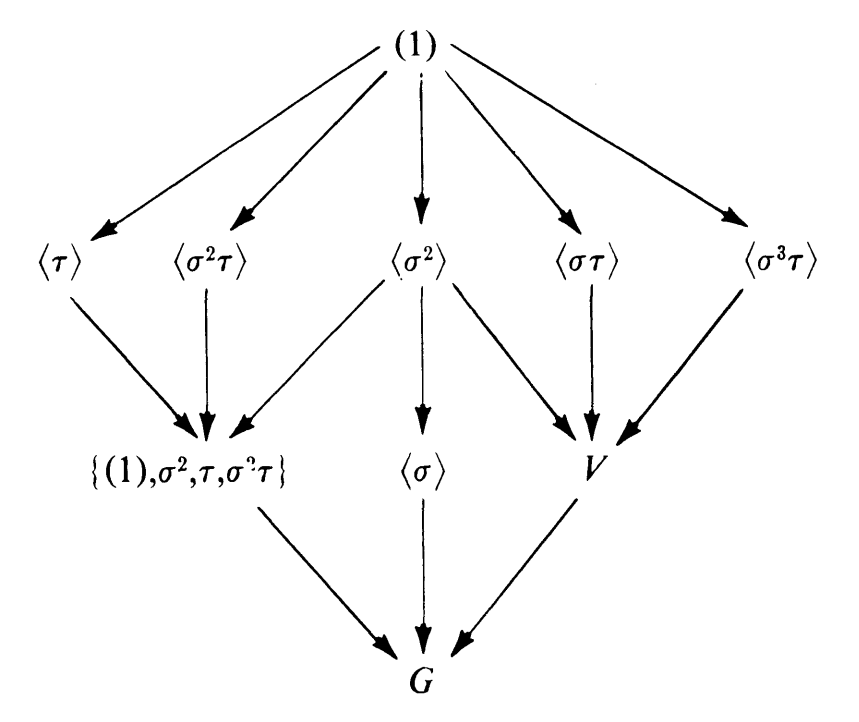
\includegraphics[scale=0.29]{Images/Subgroups.png}
    \caption{Subgroup lattice, where $H\to K$ means $H<K$}
\end{figure}
\begin{figure}[htbp]
    \center
    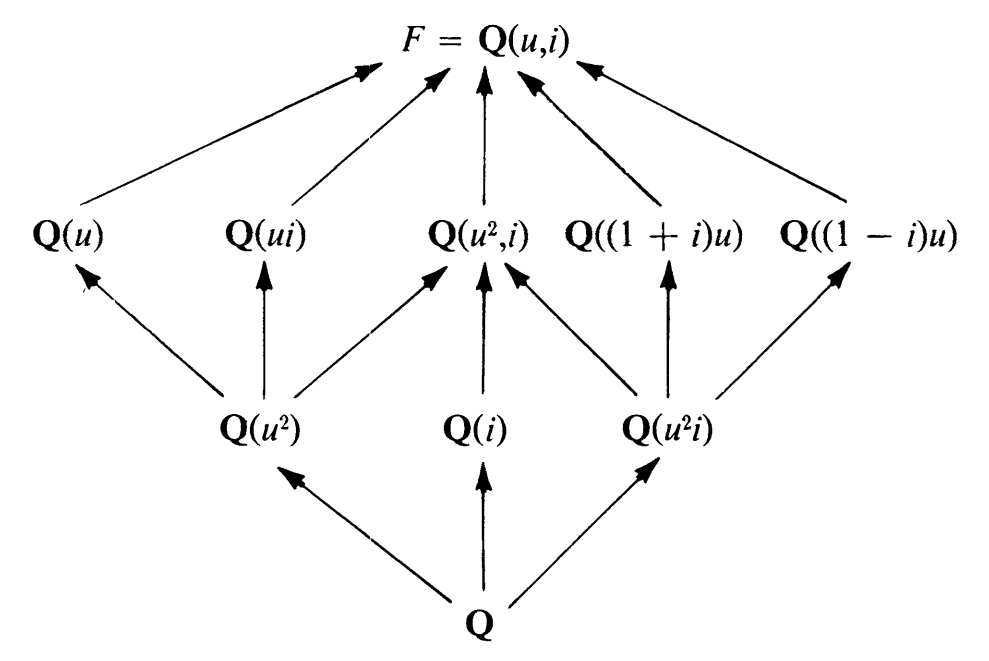
\includegraphics[scale=0.29]{Images/Intermediate Fields.png}
    \caption{Intermediate field lattice, where $M\to N$ means $M\subset N$}
\end{figure}
\end{example}
Specific techniques for computing Galois groups of polynomials of degree greater than $4$ are rather scarce. We shall we content with a very special case.
\begin{theorem}
If $p$ is prime and $f$ is an irreducible polynomial of degree $p$ over the field of rational numbers which has precisely two non-real roots in the field of complex numbers, then the Galois group of $f$ is (isomorphic to) $S_p$.
\end{theorem}
\begin{proof}
Let $G$ be the Galois group of $f$, then $p\mid |G|$. Therefore by Cauchy's theorem there exists some $\sigma\in G$ such that $\sigma$ is of order $p$. Since $\sigma\in S_n$, $\sigma$ is a $p$-cycle. Now complex conjugation is an $\mathbb{R}$-automorphism of $\mathbb{C}$ that moves every non-real elements. Therefore it interchanges the two non-real roots of $f$ and fix all others. This implies $G$ contains a transportation $\tau=(ab)$. We may suppose, by changing notation if necessary, that $\tau=(12)$ and $\sigma^k=(12\cdots p)$ for some $k$. However $\tau$ and $\sigma$ together generate $S_p$, hence $G=S_p$.
\end{proof}
\begin{center}
\begin{large}
    \textbf{Exercises for 6.4}
\end{large}
\end{center}
Unless stated otherwise $K$ is a field, $f\in K[x]$ and $F$ is a splitting field of $f$ over $K$.
\begin{problem}\em
Suppose $f\in K[x]$ splits in $F$ as $f=(x-u_1)^{n_1}\cdots (x-u_k)^{n_k}$ ($u_i$ distinct; $n_i\geq 1$). Let $v_0, ..., v_k$ be the coefficients of the polynomial $g=(x-u_1)(x-u_2)\cdots (x-u_k)$ and let $E=K(v_0, ..., v_k)$. Then \par
(i) $F$ is a splitting field of $g$ over $E$.\par
(ii) $F$ is Galois over $E$.\par
(iii) $\mathrm{Gal}(F/E)=\mathrm{Gal}(F/K)$.
\end{problem}
\begin{proof}
(i) Since $f$ splits in $F$ and $f$ and $g$ has the same roots (without counting the multiples), we have $g$ splits in $F$ and hence $F$ is a splitting field of $g$ over $E$.\par
(ii) Let $h\in E[x]$ be a polynomial in $E[x]$ that has a root in $F$. Then since $F$ is the splitting field over $E$, we have $h$ splits in $F$ and hence  $F/E$ is normal. By the definition of $E$ we have $h$ separable and hence $F/E$ is Galois.\par
(iii) Suppose $\sigma\in\mathrm{Aut}(F/K)$. Then $\sigma$ is a permutation of $\{u_1,\cdots,u_n\}$, where $u_i$ are the roots of a polynomial $g\in E[x]$. Therefore $\sigma$ actually fix $g$ and hence fix $E$. This implies $\sigma\in\mathrm{Gal}(F/E)$.
\end{proof}
\begin{problem}\em
Suppose $K$ is a subfield of $\mathbb{R}$ (so that $F$ may be taken to be a subfield of $\mathbb{C}$) and that $f$ is irreducible of degree $3$. Let $D$ be the discriminant of $f$. Then \par
(i) $D>0$ if and only if $f$ has three real roots.\par
(ii) $D<0$ if and only if $f$ has precisely one real root.
\end{problem}
\begin{proof}
We first show that if $\Delta^2>0$, then $\Delta\in\mathbb{R}$. Suppose $\Delta=a+b\mathrm{i}$, then $\Delta^2=a^2-b^2+2ab\mathrm{i}$. If $\Delta^2\in\mathbb{R}$, then $ab=0$. If $a=0$, then $\Delta^2=-b^2\le 0$, a contradiction! Therefore $\Delta=a\in\mathbb{R}$.\par
(i) Since $D=\Delta^2>0$, we have $\Delta\in\mathbb{R}$. Hence $\prod(u_i-u_j)\in\mathbb{R}$, which implies $u_i\in\mathbb{R}$.\par
(ii) Since $D=\Delta^2<0$, we have $\Delta\in\mathbb{C}-\mathbb{R}$. Hence $\prod(u_i-u_j)\in\mathbb{C}-\mathbb{R}$, which implies there exists at least one $u_i$ such that $u_i\in\mathbb{C}-\mathbb{R}$. However if there is only one such $u_i$, the square of $\Delta$ is either in $\mathbb{C}-\mathbb{R}$ or positive. Therefore there are two roots in $\mathbb{C}-\mathbb{R}$.
\end{proof}
\begin{problem}\em
Let $f$ be a separable cubic with Galois group $S_3$ and roots $u_1, u_2, u_3\in F$. Then the distinct intermediate fields of the extension of $K$ by $F$ are $F, K(\Delta), K(u_1), K(u_2), K(u_3), K$. The corresponding subgroups of the Galois group are $1, A_3, T_1, T_2, T_3$ and $S_3$ where $T_i=\{(1), (jk)\mid j\neq i\neq k\}$.
\end{problem}
\begin{proof}
Since the Galois group of $f$ is $S_3$, we have $\Delta\notin K$. Therefore we have the following Galois correspondence 
\begin{center}


\tikzset{every picture/.style={line width=0.75pt}} %set default line width to 0.75pt        

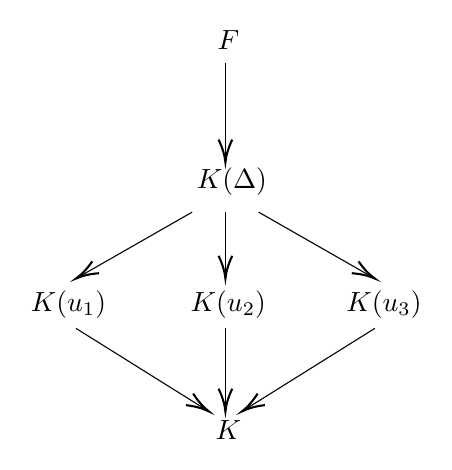
\begin{tikzpicture}[x=0.75pt,y=0.75pt,yscale=-1,xscale=1]
%uncomment if require: \path (0,476); %set diagram left start at 0, and has height of 476

%Straight Lines [id:da032329933164278346] 
\draw    (272,112) -- (272,158) ;
\draw [shift={(272,160)}, rotate = 270] [color={rgb, 255:red, 0; green, 0; blue, 0 }  ][line width=0.75]    (10.93,-3.29) .. controls (6.95,-1.4) and (3.31,-0.3) .. (0,0) .. controls (3.31,0.3) and (6.95,1.4) .. (10.93,3.29)   ;
%Straight Lines [id:da9414101801961103] 
\draw    (256,184) -- (201.74,215.01) ;
\draw [shift={(200,216)}, rotate = 330.26] [color={rgb, 255:red, 0; green, 0; blue, 0 }  ][line width=0.75]    (10.93,-3.29) .. controls (6.95,-1.4) and (3.31,-0.3) .. (0,0) .. controls (3.31,0.3) and (6.95,1.4) .. (10.93,3.29)   ;
%Straight Lines [id:da03991259947222936] 
\draw    (272,184) -- (272,214) ;
\draw [shift={(272,216)}, rotate = 270] [color={rgb, 255:red, 0; green, 0; blue, 0 }  ][line width=0.75]    (10.93,-3.29) .. controls (6.95,-1.4) and (3.31,-0.3) .. (0,0) .. controls (3.31,0.3) and (6.95,1.4) .. (10.93,3.29)   ;
%Straight Lines [id:da21039231506414402] 
\draw    (288,184) -- (342.26,215.01) ;
\draw [shift={(344,216)}, rotate = 209.74] [color={rgb, 255:red, 0; green, 0; blue, 0 }  ][line width=0.75]    (10.93,-3.29) .. controls (6.95,-1.4) and (3.31,-0.3) .. (0,0) .. controls (3.31,0.3) and (6.95,1.4) .. (10.93,3.29)   ;
%Straight Lines [id:da08651726223892764] 
\draw    (200,240) -- (262.3,278.94) ;
\draw [shift={(264,280)}, rotate = 212.01] [color={rgb, 255:red, 0; green, 0; blue, 0 }  ][line width=0.75]    (10.93,-3.29) .. controls (6.95,-1.4) and (3.31,-0.3) .. (0,0) .. controls (3.31,0.3) and (6.95,1.4) .. (10.93,3.29)   ;
%Straight Lines [id:da4999449076953608] 
\draw    (272,240) -- (272,278) ;
\draw [shift={(272,280)}, rotate = 270] [color={rgb, 255:red, 0; green, 0; blue, 0 }  ][line width=0.75]    (10.93,-3.29) .. controls (6.95,-1.4) and (3.31,-0.3) .. (0,0) .. controls (3.31,0.3) and (6.95,1.4) .. (10.93,3.29)   ;
%Straight Lines [id:da30117976366070653] 
\draw    (344,240) -- (281.7,278.94) ;
\draw [shift={(280,280)}, rotate = 327.99] [color={rgb, 255:red, 0; green, 0; blue, 0 }  ][line width=0.75]    (10.93,-3.29) .. controls (6.95,-1.4) and (3.31,-0.3) .. (0,0) .. controls (3.31,0.3) and (6.95,1.4) .. (10.93,3.29)   ;

% Text Node
\draw (267,95.4) node [anchor=north west][inner sep=0.75pt]    {$F$};
% Text Node
\draw (257,161.4) node [anchor=north west][inner sep=0.75pt]    {$K( \Delta )$};
% Text Node
\draw (177,220.4) node [anchor=north west][inner sep=0.75pt]    {$K( u_{1})$};
% Text Node
\draw (254,220.4) node [anchor=north west][inner sep=0.75pt]    {$K( u_{2})$};
% Text Node
\draw (329,220.4) node [anchor=north west][inner sep=0.75pt]    {$K( u_{3})$};
% Text Node
\draw (266,283.4) node [anchor=north west][inner sep=0.75pt]    {$K$};


\end{tikzpicture}
\end{center}
and the subgroups 
\begin{center}


\tikzset{every picture/.style={line width=0.75pt}} %set default line width to 0.75pt        

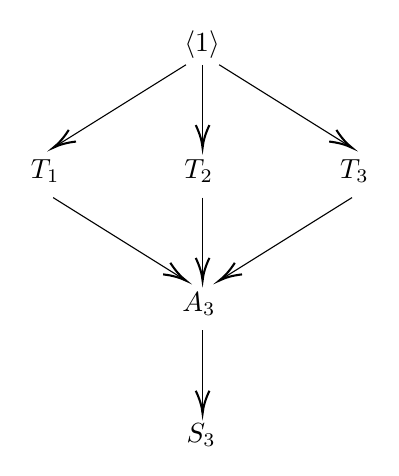
\begin{tikzpicture}[x=0.75pt,y=0.75pt,yscale=-1,xscale=1]
%uncomment if require: \path (0,476); %set diagram left start at 0, and has height of 476

%Straight Lines [id:da9414101801961103] 
\draw    (264,176) -- (201.7,214.94) ;
\draw [shift={(200,216)}, rotate = 327.99] [color={rgb, 255:red, 0; green, 0; blue, 0 }  ][line width=0.75]    (10.93,-3.29) .. controls (6.95,-1.4) and (3.31,-0.3) .. (0,0) .. controls (3.31,0.3) and (6.95,1.4) .. (10.93,3.29)   ;
%Straight Lines [id:da03991259947222936] 
\draw    (272,176) -- (272,214) ;
\draw [shift={(272,216)}, rotate = 270] [color={rgb, 255:red, 0; green, 0; blue, 0 }  ][line width=0.75]    (10.93,-3.29) .. controls (6.95,-1.4) and (3.31,-0.3) .. (0,0) .. controls (3.31,0.3) and (6.95,1.4) .. (10.93,3.29)   ;
%Straight Lines [id:da21039231506414402] 
\draw    (280,176) -- (342.3,214.94) ;
\draw [shift={(344,216)}, rotate = 212.01] [color={rgb, 255:red, 0; green, 0; blue, 0 }  ][line width=0.75]    (10.93,-3.29) .. controls (6.95,-1.4) and (3.31,-0.3) .. (0,0) .. controls (3.31,0.3) and (6.95,1.4) .. (10.93,3.29)   ;
%Straight Lines [id:da08651726223892764] 
\draw    (200,240) -- (262.3,278.94) ;
\draw [shift={(264,280)}, rotate = 212.01] [color={rgb, 255:red, 0; green, 0; blue, 0 }  ][line width=0.75]    (10.93,-3.29) .. controls (6.95,-1.4) and (3.31,-0.3) .. (0,0) .. controls (3.31,0.3) and (6.95,1.4) .. (10.93,3.29)   ;
%Straight Lines [id:da4999449076953608] 
\draw    (272,240) -- (272,278) ;
\draw [shift={(272,280)}, rotate = 270] [color={rgb, 255:red, 0; green, 0; blue, 0 }  ][line width=0.75]    (10.93,-3.29) .. controls (6.95,-1.4) and (3.31,-0.3) .. (0,0) .. controls (3.31,0.3) and (6.95,1.4) .. (10.93,3.29)   ;
%Straight Lines [id:da30117976366070653] 
\draw    (344,240) -- (281.7,278.94) ;
\draw [shift={(280,280)}, rotate = 327.99] [color={rgb, 255:red, 0; green, 0; blue, 0 }  ][line width=0.75]    (10.93,-3.29) .. controls (6.95,-1.4) and (3.31,-0.3) .. (0,0) .. controls (3.31,0.3) and (6.95,1.4) .. (10.93,3.29)   ;
%Straight Lines [id:da6118594202844929] 
\draw    (272,304) -- (272,342) ;
\draw [shift={(272,344)}, rotate = 270] [color={rgb, 255:red, 0; green, 0; blue, 0 }  ][line width=0.75]    (10.93,-3.29) .. controls (6.95,-1.4) and (3.31,-0.3) .. (0,0) .. controls (3.31,0.3) and (6.95,1.4) .. (10.93,3.29)   ;

% Text Node
\draw (262,158.4) node [anchor=north west][inner sep=0.75pt]    {$\left<1\right>$};
% Text Node
\draw (188,220.4) node [anchor=north west][inner sep=0.75pt]    {$T_{1}$};
% Text Node
\draw (262,220.4) node [anchor=north west][inner sep=0.75pt]    {$T_{2}$};
% Text Node
\draw (337,220.4) node [anchor=north west][inner sep=0.75pt]    {$T_{3}$};
% Text Node
\draw (261,284.4) node [anchor=north west][inner sep=0.75pt]    {$A_{3}$};
% Text Node
\draw (263,347.4) node [anchor=north west][inner sep=0.75pt]    {$S_{3}$};


\end{tikzpicture}
\end{center}
\end{proof}
\begin{problem}\em
If $\mathrm{char }K\neq 2, 3$ then the discriminant of $x^3+bx^2+cx+d$ is $-4c^3-27d^2+b^2(c^2-4bd)+18bcd$.
\end{problem}
\begin{proof}
This follows from a direct computation. Note that $\mathrm{char}K\ne 2,3$, hence the coefficients in the discriminant is valid.
\end{proof}
\begin{problem}\em
If $\mathrm{char }K\neq 2$ and $f\in K[x]$ is a cubic whose discriminant is a square in $K$, then $f$ is either irreducible or factors completely in $K$.
\end{problem}
\begin{proof}
Suppose $f$ is reducible in $K[x]$. Then there exists some $u\in K$ such that $u$ is a root of $f$. Note that the discriminant of $f$ is a square of $K$, therefore the Galois group of $f$ is $S_4$, hence there exists some permutations $\sigma$ such that $\sigma^k(u)$ consists of all root of $f$ when $k$ run over integers. Therefore $f$ splits in $K$ and hence factors completely in $K$.
\end{proof}
\begin{problem}\em
Over any base field $K$, $x^3-3x+1$ is either irreducible or splits over $K$.
\end{problem}
\begin{proof}
We compute the discriminant of the polynomial as follows: 
$$
D=\Delta ^2=-4\left( -3 \right) ^3-27=81=9^2,
$$
and since $\mathbb{Q}$ is the smallest number field we have $\mathbb{Q}\subset K$, hence $\Delta\in K$. Therefore by Exercise 6.51 we have $x^3-3x+1$ is either irreducible or splits over $K$.
\end{proof}
\begin{problem}\em
$S_4$ has no transitive subgroup of order $6$.
\end{problem}
\begin{proof}
We characterize the subgroups of order $6$ of $S_4$. Since the group of order $6$ must contain s Sylow $3$-subgroup, it is generated by a $3$-cycle and a $2$-cycle. Therefore all subgroups of $S_4$ of order $6$ is of the form $\{(ij)(ijk)\}$, where $\{i,j,k\}\subset\{1,2,3,4\}$. No such subgroups are transitive.
\end{proof}
\begin{problem}\em
Let $f$ be an (irreducible) separable quartic over $K$ and $u$ a root of $f$. There is no field properly between $K$ and $K(u)$ if and only if the Galois group of $f$ is either $A_4$ or $S_4$.
\end{problem}
\begin{proof}
Note that $[K(u):K]=4$. If there is a proper intermediate field $E$, then $[K(u):E]=[E:K]=2$. Therefore we have the following correspondence: 
$$
\begin{matrix}
	K&		\mapsto&		G\\
	\cap&		&		\land\\
	E&		\mapsto&		H\\
	\cap&		&		\land\\
	K\left( u \right)&		\mapsto&		L\\
	\cap&		&		\land\\
	K&		\mapsto&		1\\
\end{matrix}
$$
If $m=1$, then $G\cong V\cong\mathbb{Z}_2\oplus\mathbb{Z}_2$. Take $H=\mathbb{Z}_2\oplus\{0\}$ and $L=\{0\}$.\par
If $m=2$, then $G\cong D_4$ or $G\cong\mathbb{Z}_4$. If $G\cong D_4$, then take $H=\left<(ij)\right>$ and $L=\{0\}$. Otherwise take $H=\mathbb{Z}_2$ and $L=\{0\}$.\par
If $m=3$, then $G\cong A_4$. However there are no subgroups of $A_4$ of order $2$.\par
If $m=6$, then $G\cong S_4$. Then the only possible $H$ is $A_4$, however $A_4$ has no subgroups of order $2$.\par
Therefore if there exists some such intermediate fields, we have $m=1$ or $m=2$. Therefore there are no field properly between $K$ and $K(u)$ if and only if $m=3$ or $m=6$, i.e. the Galois group of $f$ is either $A_4$ or $S_4$.
\end{proof}
\begin{problem}\em
Let $x^4+ax^2+b\in K[x]$ (with $\mathrm{char }K\neq 2$) be irreducible with Galois group $G$.\par
(i) If $b$ is a square in $K$, then $G=V$.\par
(ii) If $b$ is not a square in $K$ and $b(a^2-4b)$ is a square in $K$, then $G\cong \mathbb{Z}_4$.\par
(iii) If neither $b$ nor $b(a^2-4b)$ is a square in $K$, then $G\cong D_4$.
\end{problem}
\begin{proof}
Note that the resolvant cubic of the polynomial $x^4+ax^2+b$ is $x^3-ax^2-4bx+4ab=(x-a)(x+2\sqrt{b})(x-2\sqrt{b})$. \par
(i) If $b$ is a square in $K$, then $m=1$, hence $G=V$.\par
(ii) If $b$ is not a square in $K$, note that $K(\alpha,\beta,\gamma)=K(\sqrt{b})$, we have $m=2$. Also note that 
$$
\begin{aligned}
x^4+ax^2+b&=\left( x^2-\frac{-a+\sqrt{a^2-4b}}{2} \right) \left( x^2-\frac{-a-\sqrt{a^2-4b}}{2} \right) 
\\
&=\left( x+\sqrt{\frac{-a+\sqrt{a^2-4b}}{2}} \right) \left( x-\sqrt{\frac{-a+\sqrt{a^2-4b}}{2}} \right) \left( x+\sqrt{\frac{-a-\sqrt{a^2-4b}}{2}} \right) \left( x-\frac{-a-\sqrt{a^2-4b}}{2} \right) ,
\end{aligned}
$$
it suffices to show that the four root actually lie in $K(\sqrt{b})$. Since $b(a^2-4b)$ is a square in $K$, we may suppose $\sqrt{a^2-4b}=t\sqrt{b}$ for some $t\in K$. Therefore 
$$
\sqrt{\frac{-a+\sqrt{a^2-4b}}{2}}=\sqrt{-\frac{a}{2}+\frac{t}{2}\sqrt{b}}=m+n\sqrt{b}
$$
for some $m,n\in K$, hence $x^4+ax^2+b$ is factored in $K(\sqrt{b})$, therefore $G=\mathbb{Z}_4$.\par
(iii) If $b(a^2-4b)$ is not a square in $K$, then $x^4+ax^2+b$ can't be factored in $K(\sqrt{b})$ and hence $G\cong D_4$.
\end{proof}
\begin{problem}\em
Determine all the subgroups of the Galois group and all of the intermediate fields of the splitting field (over $\mathbb{Q}$) of the polynomial $x^4-5\in \mathbb{Q}[x]$.
\end{problem}
\begin{proof}
Trivially the splitting field over $\mathbb{Q}$ of the polynomial $x^4-5$ is $\mathbb{Q}(\mathrm{i},\sqrt[4]{5})$. Let $\tau$ be the complex conjugation and $\sigma$ the rotation given by $z\mapsto\mathrm{i}z$, then we have the following diagram of intermediate fields 
$$
\begin{matrix}
	&		&		&		&		\mathbb{Q} (\mathrm{i},\sqrt[4]{5})&		&		\\
	&		&		&		\swarrow&		\downarrow&		\searrow&		\\
	&		&		\mathbb{Q} (\mathrm{i},\sqrt{5})&		&		\mathbb{Q} (\sqrt[4]{5})&		&		\mathbb{Q} (\mathrm{i}\sqrt[4]{5})\\
	&		\swarrow&		\downarrow&		\searrow&		\downarrow&		\swarrow&		\\
	\mathbb{Q} (\mathrm{i)}&		&		\mathbb{Q} (\mathrm{i}\sqrt{5})&		&		\mathbb{Q} (\sqrt{5})&		&		\\
	&		\searrow&		\downarrow&		\swarrow&		&		&		\\
	&		&		\mathbb{Q}&		&		&		&		\\
\end{matrix}
$$
and subgroups 
$$
\begin{matrix}
	&		&		&		&		\{1\}&		&		\\
	&		&		&		\swarrow&		\downarrow&		\searrow&		\\
	&		&		\langle \sigma ^2\rangle&		&		\langle \tau \rangle&		&		\langle \tau \sigma ^2\rangle\\
	&		\swarrow&		\downarrow&		\searrow&		\downarrow&		\swarrow&		\\
	\langle \sigma \rangle \cong \mathbb{Z} _4&		&		\langle \tau \sigma ,\sigma ^2\rangle \cong V&		&		\langle \tau ,\sigma ^2\rangle \cong V&		&		\\
	&		\searrow&		\downarrow&		\swarrow&		&		&		\\
	&		&		\langle \tau ,\sigma \rangle \cong D_4&		&		&		&		\\
\end{matrix}
$$
\end{proof}
\begin{problem}\em
Let $K$ be a subfield of the real numbers and $f\in K[x]$ an irreducible quartic. If $f$ has exactly two real roots, the Galois group of $f$ is $S_4$ or $D_4$.
\end{problem}
\begin{proof}
Since the polynomial has two real roots, the complex conjugation $\sigma$ lies in the Galois group of $f$. Note that $f$ is irreducible, the Galois group of $f$ is transitive. Hence the only candidates are $S_4$, $A_4$, $D_4$, $\mathbb{Z}_4$ and $\mathbb{Z}_2\oplus\mathbb{Z}_2$. However $\sigma$ is an odd permutation, therefore $\sigma\notin A_4$, so not in the subgroup $\mathbb{Z}_4$ of $A_4$. For $\mathbb{Z}_2\oplus\mathbb{Z}_2$, note that $\mathbb{Z}_2\oplus\mathbb{Z}_2=\{e,(12)(34),(13)(24),(14)(23)\}$, which does not contain a transposition.
\end{proof}
\subsection{Finite Fields}
In this section finite fields (sometimes called \textbf{Galois fields}) are characterized in terms of splitting fields and their structure completely determined. We begin with two theorems and a lemma that apply to fields which need not be finite. In each case, of course, we are interested primarily in the implications for finite fields.
\begin{theorem}
Let $F$ be a field and let $P$ be the intersection of all subfields of $F$. Then $P$ is a field with no proper subfields. If $\mathrm{char}F=p$ is a prime, then $P\cong\mathbb{Z}_p$. If $\mathrm{char}F=0$, then $P\cong\mathbb{Q}$, the field of rational numbers.
\end{theorem}
\begin{note}\em
The field $P$ is called the \textbf{prime subfield} of $F$.
\end{note}
\begin{proof}
We first show that $P$ is a subfield of $F$. Since $0$ and $1_F$ must lie in $P$, $P$ is nonempty. Suppose $x,y\in P$, then $x,y\in E$ for all $E$ a subfield of $F$. Therefore $x-y\in E$ and $x^{-1}y\in E$ for all $E\subset F$, hence $P=\bigcap E$ is also a field. Now if $E$ is a subfield of $F$, then by definition of $P$ we have $E\cap P=E$, hence $E=P$ and $P$ is the smallest subfield of $F$.\par
Now suppose $\mathrm{char}F=p$. Consider the map $\varphi:\mathbb{Z}\to P$ given by $m\mapsto m1_F$, then $\mathrm{Ker}\varphi=(p)$ and hence $\mathrm{Im}\varphi\cong\mathbb{Z}/(p)=\mathbb{Z}_p$. Since $\mathrm{Im}\varphi$ is a subfield of $P$, we have $\mathrm{Im}\varphi=P$ and hence $P\cong\mathbb{Z}_p$. Similarly we may prove $P\cong\mathbb{Q}$ when $\mathrm{char}F=0$.
\end{proof}
\begin{corollary}
If $F$ is a finite field, then $\mathrm{char}F=p\ne 0$ for some prime $p$, and $|F|=p^n$ for some integer $n\ge 1$.
\end{corollary}
\begin{proof}
Since $F$ is finite, the prime subfield of $F$ is finite and hence not isomorphic to $\mathbb{Q}$. Therefore $\mathrm{char}F\ne 0$. Since $F$ is a field, we therefore conclude that $\mathrm{char}F=p$ for some prime $p$. Now since $F$ is a finite dimensional vector space over $\mathbb{Z}_p$, we have $F\cong\mathbb{Z}_p\oplus\cdots\oplus\mathbb{Z}_p$ and hence $|F|=p^n$ for some $n\ge 1$.
\end{proof}
In the sequel we shall always identity the prime subfield of a field as $\mathbb{Z}_p$ or $\mathbb{Q}$ under the isomorphism given in Theorem 6.52. For instance, we shall write $\mathbb{Z}_p\subset F$, and $1_F=1\in\mathbb{Z}_p$.
\begin{theorem}
If $F$ is a field and $G$ is a finite subgroup of the multiplicative group of nonzero elements of $F$, then $G$ is a cyclic group. In particular, the multiplicative group of all nonzero elements of finite fields is cyclic.
\end{theorem}
\begin{proof}
Suppose $G\cong\mathbb{Z}_{m_1}\oplus\mathbb{Z}_{m_2}\oplus\cdots\oplus\mathbb{Z}_{m_k}$ and $m_1\mid m_2\mid\cdots\mid m_k$, or otherwise the condition is trivial. Therefore $m_k\left(\bigoplus_{i=1}^k\mathbb{Z}_{m_i}\right)=0$, it follows that every $u\in G$ is a root of $x^{m_k}-1_F\in F[x]$. Note that the polynomial has at most $m_k$ distinct roots in $F$, we have $G\cong\mathbb{Z}_{m_k}$.
\end{proof}
\begin{corollary}
If $F$ is a finite field, then $F$ is a simple extension of its prime subfield $\mathbb{Z}_p$, that is, $F=\mathbb{Z}_p(u)$ for some $u\in F$.
\end{corollary}
\begin{proof}
Let $u$ be the generator of the multiplicative group of nonzero elements of $F$.
\end{proof}
\begin{lemma}\em
If $F$ is a field of characteristic $p$ and $r\ge 1$ is an integer, then the map $\varphi:F\to F$ given by $u\mapsto u^{p^r}$ is a $\mathbb{Z}_p$-monomorphism of fields. If $F$ is finite, then $\varphi$ is a $\mathbb{Z}_p$-automorphism of $F$.
\end{lemma}
\begin{proof}
Note that in the field of characteristic $p$ we have $(u+v)^p=u^p+v^p$, therefore if $u^{p^r}=v^{p^r}$, we have $u^{p^r}-v^{p^r}=(u-v)^{p^r}=0$, hence $u-v=0$ and $u=v$. Therefore $\varphi$ is a monomorphism. Now if $k\in\mathbb{Z}_p$, we have $k^{p^r}=k$ and hence $\varphi$ fix $\mathbb{Z}_p$.
\end{proof}
We can now give a useful characterization of finite fields.
\begin{proposition}
Let $p$ be a prime and $n\ge 1$ an integer. Then $F$ is a finite field with $p^n$ elements if and only if $F$ is a splitting field of $x^{p^n}-x$ over $\mathbb{Z}_p$.
\end{proposition}
\begin{proof}
If $|F|=p^n$, then the multiplicative group of nonzero elements of $F$ has order $p^n-1$ and hence every nonzero element $u\in F$ satisfies $u^{p^n-1}=1_F$. Therefore $u$ is a root of $x^{p^n-1}-1_F$ and therefore a root of $x(x^{p^n-1}-1_F)=x^{p^n}-x$. Since $0\in F$ is also a root of $x^{p^n}-x$, we have $x^{p^n}-x$ splits in $F$ and hence $F$ is a splitting field over $\mathbb{Z}_p$ of the polynomial $x^{p^n}-x$.\par
Conversely, suppose $x^{p^n}-x$ splits in $F$. Note that $x^{p^n}-x$ has $p^n$ distinct elements in $F$. If $\varphi$ is the monomorphism as defined in Lemma 6.15, we have $u$ is a root of $x^{p^n}-x$ if and only if $\varphi(u)=u$. Let $E$ be the set of all $u\in F$ such that $\varphi(u)=u$. Therefore suppose $u$ and $v\in E$ , we have $(u+v)^{p^n}=u+v$, $(uv)^{p^n}=uv$ and $(u^{-1})^{p^n}=u^{-1}$, therefore the set of all such $u$ that $\varphi(u)=u$ is a field of order $p^n$, and hence $F=\mathbb{Z}_p(E)=E$.
\end{proof}
\begin{corollary}
If $p$ is a prime and $n\ge 1$ an integer, then there exists a field with $p^n$ elements. Any two finite fields with the same number of elements are isomorphic.
\end{corollary}
\begin{proof}
To show the existence, consider a splitting field over $\mathbb{Z}_p$ of the polynomial $x^{p^n}-x$. Note that any field of order $p^n$ is a splitting field over $\mathbb{Z}_p$ of the polynomial $x^{p^n}-x$, we have any two finite fields with the same number of elements are isomorphic.
\end{proof}
\begin{corollary}
If $K$ is a finite field and $n\ge 1$ is an integer, then there exists a simple extension field $F=K(u)$ of $K$ such that $F$ is finite and $[F:K]=n$. Any two $n$-dimensional extension fields of $K$ are $K$-isomorphic.
\end{corollary}
\begin{proof}
Given $K$ of order $p^r$. Let $F$ be a splitting field over $K$ of $f=x^{p^{nr}}-x$. Note that for all $u\in K$, we have $u^{p^r}=u$, hence by induction we have $u^{p^{rn}}=u$. Therefore $K$ is the field of $\mathbb{Z}_p$ adjoined with \textit{some} roots of $f$. Therefore by Exercise 6.31 we have $F/\mathbb{Z}_p$ is a splitting field of $f$. Hence $F$ consists of precisely the $p^{nr}$ roots of $f$. Therefore $p^{nr}=\left| F \right|=\left| K \right|^{\left[ F:K \right]}=\left( p^r \right) ^{\left[ F:K \right]}$, hence $[F:K]=n$. By Corollary 6.55 we know that $F$ is a simple extension of $K$.\par
Now if there is another extension field $F_1$ such that $[F_1:K]=n$, then $[F_1:\mathbb{Z}_p]=[F_1:K][K:\mathbb{Z}_p]=p^{nr}$, hence $F_1$ is a splitting field over $\mathbb{Z}_p$ of $f$ and hence $F_1\cong F$.
\end{proof}
\begin{corollary}
If $K$ is a finite field and $n\ge 1$ an integer, then there exists an irreducible polynomial of degree $n$ in $K[x]$.
\end{corollary}
\begin{proof}
If there were no such irreducible polynomials, then for all $u\in\overline{K}$ we have $[K(u):K]\ne n$. However by Corollary 6.28 there exists some $u$ such that $[K(u):K]=n$, a contradiction!
\end{proof}
\begin{proposition}
If $F$ is a finite dimensional extension field of a finite field $K$, then $F$ is finite and is Galois over $K$. The Galois group $\mathrm{Gal}(F/K)$ is cyclic.
\end{proposition}
\begin{proof}
Let $\mathbb{Z}_p$ be the prime subfield of $K$. Then $F$ is a finite dimensional over $\mathbb{Z}_p$. Suppose $[F:\mathbb{Z}_p]=n$, then $|F|=p^n$. By Proposition 6.56 $F$ is a splitting field over $\mathbb{Z}_p$ of the polynomial $x^{p^n}-x$, hence a splitting field over $K$. Since the zeros of the polynomial $x^{p^n}-x$ are distinct, we have $F/K$ is separable and hence $F/K$ a Galois extension. By Lemma 6.15 the map $\varphi:F\to F$ given by $u\mapsto u^p$ is a $\mathbb{Z}_p$-automorphism. Clearly $\varphi^n$ is the identity map and $n$ is the least positive integer $k$ such that $\varphi^k$ is an identity. Since $|\mathrm{Aut}(G/\mathbb{Z}_p)|=n$ by the Fundamental theorem, we have $|\mathrm{Aut}(G/\mathbb{Z}_p)|$ is generated by $\varphi$, which is cyclic. Note that the subgroup of a cyclic group is cyclic, we have $\mathrm{Gal}(F/K)$ cyclic.
\end{proof}
\begin{center}
\begin{large}
    \textbf{Exercises for 6.5}
\end{large}
\end{center}
$F$ always denotes an extension field of a field $K$.
\begin{problem}\em
If $K$ is a finite field of characteristic $p$, describe the structure of the additive group of $K$.
\end{problem}
\begin{proof}
Since $K$ is a finite field of characteristic $p$, we have $|K|=p^m$ for some $m=[K:\mathbb{Z}_p]$. Therefore $K$ may be seen as a $m$-dimensional vector space over $\mathbb{Z}_p$, hence we have $K\cong\mathbb{Z}_p\oplus\mathbb{Z}_p\oplus\cdots\oplus\mathbb{Z}_p$ ($m$ summonds). Therefore we obtain the structure of the additive group $(K,+)=(\mathbb{Z}_p^m,+)$.
\end{proof}
\begin{problem}\em
(Fermat) If $p\in \mathbb{Z}$ is prime, then $a^p=a$ for all $a\in \mathbb{Z}_p$ or equivalently, $c^p\equiv c\pmod{p}$ for all $c\in \mathbb{Z}$.
\end{problem}
\begin{proof}
Consider $\mathbb{Z}_p$ as the splitting field of the polynomial $x^p-x$. Therefore we have for all $a\in\mathbb{Z}_p$ we have $a^p-a=0$. Therefore $a^p=a$ in $\mathbb{Z}_p$ and $c^p\equiv c(\mathrm{mod}\ p)$ for all $c\in\mathbb{Z}$.
\end{proof}
\begin{problem}\em
If $|K|=p^n$, then every element of $K$ has a unique $p$th root in $K$.
\end{problem}
\begin{proof}
Suppose $\alpha\in K$. We consider the polynomial $x^p-\alpha$. Since the derivative of $x^p-\alpha$ is zero, it has multiple roots. Indeed suppose $\beta$ is a root of $x^p-\alpha$, we have $(x-\beta)^p=x^p-\beta^p=x^p-\alpha$, hence $\beta$ is the only root of $x^p-\alpha$ without counting multiples. Now we show that $\beta\in K$. Consider the mapping $\alpha\mapsto\alpha^p$, by Lemma 6.15 and the fact that $K$ is a finite field we have the mapping is an automorphism, hence $\alpha^p\in K$.
\end{proof}
\begin{problem}\em
If the roots of a monic polynomial $f\in K[x]$ (in some splitting field of $f$ over $K$) are distinct and form a field, then $\mathrm{char}K=p$ and $f=x^{p^n}-x$ for some $n\geq 1$.
\end{problem}
\begin{proof}
Suppose $F$ is a splitting field over $K$ of $f$. Then $F\supset E\supset K$, where $E$ is the set of all root of $f$. Now since $F/E$ is a splitting field over $E$, we have $F=E$. Since $E$ is a finite field, we may suppose $|E|=p^n$ for some prime $p$ and $n\in\mathbb{N}$. Therefore $|E|=|K|^{[E:K]}$ implies $|K|=p$ and $[E:K]=n$. This gives $\mathrm{char}K=p$, $K=\mathbb{Z}_p$ and $f=x^{p^n}-x$, $n\ge 1$.
\end{proof}
\begin{problem}\em
Construct a field with $9$ elements and give its addition and multiplication tables.
\end{problem}
\begin{proof}
An example of a field with $9$ elements is $\mathbb{Z}_3\oplus\mathbb{Z}_3\oplus\mathbb{Z}_3$. We omit the addition and multiplication tables.
\end{proof}
\begin{problem}\em
If $|K|=q$ and $\gcd{(n, q)}=1$ and $F$ is a splitting field of $x^n-1_K$ over $K$, then $[F:K]$ is the least positive integer $k$ such that $n\mid (q^k-1)$.
\end{problem}
\begin{proof}
We first show that $n\mid(q^k-1)$. Since $F$ is a splitting field of the polynomial $x^n-1_K$ over $K$, we have $|F|=|K|^{[F:K]}=q^k$. Consider $F^\times=F-\{0\}$, then $|F^\times|=q^k-1$. Note that there exists some $u\in F^\times$ such that $u^n=1_K$, hence $u$ is an element of order $n$. Therefore by Cauchy's theorem we have $n\mid|F^\times|=q^k-1$.\par
To show that $k$ is the least element such that $n\mid(q^k-1)$, suppose there exists another $j<k$ satisfy $n\mid(q^j-1)$. Then there exists a finite field $E$ of order $q^j$ that contain an element $v$ of order $n$. Therefore $v$ is a root of $x^n-1_K$ and hence $E$ a splitting field of $x^n-1$ over $K$. However by the uniqueness of splitting fields, we have $j=k$, a contradiction!
\end{proof}
\begin{problem}\em
If $|K|=q$ and $f\in K[x]$ is irreducible, then $f$ divides $x^{q^n}-x$ if and only if $\deg{f}$ divides $n$.
\end{problem}
\begin{proof}
Suppose first $f\mid h$, where $h=x^{q^n}-x$. We suppose $\mathrm{deg}f=d$. Since $h$ splits in $\mathbb{Z}_{q^n}$, we have $f$ splits in $\mathbb{Z}_{q^n}$. Suppose $\alpha$ is a root of $f$, then $\alpha\in\mathbb{Z}_{q^n}$ and $\mathbb{Z}_q(\alpha):\mathbb{Z}_q]=d$. Therefore $n=[\mathbb{Z}_{q^n}:\mathbb{Z}_q]=[\mathbb{Z}_{q^n}:\mathbb{Z}_q(\alpha)][\mathbb{Z}_{q}(\alpha):\mathbb{Z}_q]=[\mathbb{Z}_{q^n}:\mathbb{Z}_q(\alpha)]d$, hence $d\mid n$. Conversely, suppose $d\mid n$. Say $n=pd$ for some $p$. We consider the quotient field (it is a field since $f$ is irreducible over $\mathbb{Z}_q$) $\mathbb{Z}_q[x]/(f)\cong\mathbb{Z}_{q^d}$, where the isomorphism follows from identifying $\mathbb{Z}_{p^d}$ as a simple extension of $\mathbb{Z}_p$ adjoining a root of $h$. Therefore suppose $x+(f)\in\mathbb{Z}_q[x]/(f)$, we have $(x+(f))^{q^n}=(x+(f))^{q^{pd}}=x+(f)$. Hence $x^{q^n}-x\in (f)$ and $f\mid h$.
\end{proof}
\begin{problem}\em
If $|K|=p^r$ and $|F|=p^n$, then $r\mid n$ and $\mathrm{Aut}_K F$ is cyclic with generator $\varphi$ given by $u\mapsto u^{p^r}$.
\end{problem}
\begin{proof}
Note that $[F:\mathbb{Z}_p]=n$ and $[K:\mathbb{Z}_p]=r$, we have $[F:K]=n/r\in\mathbb{Z}$, whence $r\mid n$. Now since any finite extension of finite fields are Galois, we have $|\mathrm{Gal}(F/K)|=[F:K]$ is a cyclic group as a subgroup of $\left<\phi\right>$, where $\phi:u\mapsto u^p$. Therefore $\mathrm{Gal}(F/K)=\left<\varphi\right>$ with $\varphi:u\mapsto u^{p^r}$.
\end{proof}
\begin{problem}\em
If $n\geq 3$, then $x^{2^n}+x+1$ is reducible over $\mathbb{Z}_2$.
\end{problem}
\begin{proof}
We observe that 
$$
\begin{aligned}
x^{2^n}+x+1&=\left( x^{2^n}+x^{2^{n-1}}+1 \right) +\left( x^{2^{n-1}}+x^{2^{n-2}}+1 \right) +\cdots +\left( x^2+x+1 \right) 
\\
&=\sum_{k=0}^{n-1}{\left( x^{2^{k+1}}+x^{2^k}+1 \right)}=\sum_{k=0}^{n-1}{\left( x^2+x+1 \right) ^{2^k}}
\\
&=\left( x^2+x+1 \right) \left( \sum_{k=0}^{n-1}{\left( x^2+x+1 \right) ^{2^k-1}} \right) ,
\end{aligned}
$$
therefore $x^2+x+1\mid x^{2^n}+x+1$ in $\mathbb{Z}_2$.
\end{proof}
\begin{problem}\em
Every element in a finite field may be written as the sum of two squares.
\end{problem}
Since any finite field has order $p^n$ with $p$ prime. Since $\mathbb{Z}_{p^n}\cong\mathbb{Z}\oplus\cdots\oplus\mathbb{Z}$ ($n$ summands), it suffices to prove for $\mathbb{Z}_p$. If $p=2$, trivial. We now prove the condition of $p\ge 3$.\par
Consider $S=\{x^2:x\in\mathbb{Z}_p\}$. For $k\in\mathbb{Z}_p$, we define $S(k)=\{k-x^2:x\in\mathbb{Z}_p\}$. Note that the map $x\mapsto x^2$ is a two-to-one endomorphism of $\mathbb{Z}_p^\times$ (since for all $x\in\mathbb{Z}_p$, we have $(p-x)^2=p^2-2px+x^2=x^2$ and hence the image of $x$ and $p-x$ coincide), we have $|S|=\frac{p+1}{2}$. Therefore there exists some $x^2\in S$ and $k-y^2\in S(k)$ such that $x^2=k-y^2$, which is $x^2+y^2=k$.
\subsection{Separability}
Our study of separability will be greatly facilitated by the simultaneous consideration of an concept that is, in a sense, the complete opposite of separability.
\begin{definition}
Let $F$ be an extension field of $K$. An algebraic element $u\in F$ is \textbf{purely inseparable} over $K$ if its irreducible polynomial $f$ in $K[x]$ factors in $F[x]$ as $f=(x-u)^m$. $F$ is a \textbf{purely inseparable extension} of $K$ if every element of $F$ is purely inseparable over $K$.
\end{definition}
Thus $u$ is separable over $K$ if its irreducible polynomial $f$ of degree $n$ has $n$ distinct roots in some splitting field of $K$, and purely inseparable over $K$ if $f$ has precisely one root. It is clearly possible that an element is either separable and purely inseparable over $K$.
\begin{theorem}
Let $F$ be an extension field of $K$. Then $u\in F$ is both separable and purely inseparable over $K$ if and only if $u\in K$.
\end{theorem}
\begin{proof}
Suppose $u\in F$ is both separable and purely inseparable. Then the irreducible polynomial of $u$ is of the form 
$$
f\left( x \right) =\prod_{i=1}^n{\left( x-u_i \right)}=\left( x-u \right) ^m.
$$
Therefore $f(x)=x-u$ and hence $u\in K$. Conversely, if $u\in K$, then the irreducible polynomial of $f=x-u\in K[x]$. Hence $u$ is both separable and purely inseparable.
\end{proof}
If $\mathrm{char}K=0$, then every irreducible polynomial over $K$ is separable. Therefore the only elements that are purely inseparable over $K$ are the elements of $K$ itself. Consequently we shall now consider the condition $\mathrm{char}K=p$. In order to characterize purely inseparable extensions we need 
\begin{lemma}\em
Let $F$ be an extension field of $K$ with $\mathrm{char}K=p\ne 0$. If $u\in F$ is separable over $K$, then $u^{p^n}$ is separable over $K$ for some $n\ge 0$.
\end{lemma}
\begin{proof}
We prove by induction. Suppose $u\in F$ is of degree one, then the conclusion follows trivially. Now suppose $\mathrm{deg}u=n>1$. Then the irreducible polynomial $f$ of $u$ has degree greater than one and $f^\prime(u)=0$, which implies that $f$ is a polynomial of $x^p$, whence we may regard $f$ as a polynomial of $x^p$ of degree less than $n$. Therefore by our induction hypothesis we have $(u^p)^{p^m}$ is separable over $K$ for some $m\ge 0$.
\end{proof}
\begin{theorem}
If $F$ is an algebraic extension field of a field $K$ of characteristic $p\ne 0$, then the following statements are equivalent:\par
(i) $F$ is purely inseparable over $K$;\par
(ii) The irreducible polynomial of any $u\in F$ is of the form $x^{p^n}-a\in K[x]$;\par
(iii) If $u\in F$, then $u^{p^n}\in K$ for some $n\ge 0$;\par
(iv) The only elements of $F$ which are separable over $K$ are the elements of $K$ itself;\par
(v) $F$ is generated over $K$ by a set of purely inseparable elements.
\end{theorem}
\begin{proof}
We first show that the first three statements are equivalent.\par
(i)$\Rightarrow$(ii): This is the most tricky part. The rest proof of this theorem is rather trivial. Suppose $u\in F$. Since $F$ is a purely inseparable extension field of $K$, we have the irreducible polynomial of $u$ is $f=(x-u)^m$. Suppose $m=np^r$, where $(n,p)=1$. Then $f=(x^{p^r}-u^{p^r})^n$. Since $f\in K[x]$, the coefficient of $x^{p^r(n-1)}$ lies in $K$, and hence $\pm nu^{p^r}\in K$. We claim that $u^{p^r}\in K$. Suppose $u^{p^r}=v$. Since $(p,n)=1$, by Bezout's theorem we have $kp+ln=1$ for some $k,l\in\mathbb{Z}$. Therefore $kpv+lnv=v$. Now $lnv\in K$ and $kpv=0$ since $\mathrm{char}K=p$, hence $v\in K$. Therefore $f=(x^{p^r}-v)^n$ and $u$ is purely inseparable, this is to say $n=1$ and hence $f=x^{p^r}-v$.\par
(ii)$\Rightarrow$(iii): Suppose $u\in F$, then the irreducible polynomial of $u$ is $x^{p^n}-a$ for some $a\in K$. Therefore $u^{p^n}\in K$ for some $n$.\par
(iii)$\Rightarrow$(i): Suppose $u\in F$, then there exists some $n\in\mathbb{Z}_+$ such that $u^{p^n}\in K$. Therefore $f=(x-u)^{p^n}$ has a root $u$. We may select the least $n$ such that $u^{p^n}\in K$, and hence such $f$ is irreducible and the irreducible polynomial of $f$. Therefore $u$ is purely inseparable over $K$.\par
(i)$\Rightarrow$(iv): Suppose $u\in F$. Then $u$ is purely inseparable over $K$. Now if $u$ is separable over $K$, we have $u$ being both purely inseparable and separable over $K$, hence $u\in K$.\par
(iv)$\Rightarrow$(iii): Suppose $u\in F$. By Lemma 6.16 we know that there exists some $n\ge 0$ such that $u^{p^n}$ is separable over $K$. However the only elements that are separable over $K$ are the elements of $K$ itself, hence $u^{p^n}\in K$.\par
(i)$\Rightarrow$(v): Let $X$ be the set of all purely inseparable elements in $F$ over $K$, then $F=K(X)$.\par
(v)$\Rightarrow$(iii): If $u$ is purely inseparable over $K$, then $u\in K(x_1,\cdots,x_m)$ for some $x_i$ purely inseparable over $K$, therefore $u=\sum k_ix_i$ and hence $u$ is also inseparable.
\end{proof}
\begin{corollary}
If $F$ is a finite dimensional purely inseparable extension field of $K$ and $\mathrm{char}K=p\ne 0$, then $[F:K]=p^n$ for some $n\ge 0$.
\end{corollary}
\begin{proof}
Suppose $F=K(u_1,\cdots,u_m)$, where each $u_i$ is purely inseparable over $K$. Then $u_i$ is purely inseparable over $K(u_1,\cdots,u_{i-1})$ by definition of purely inseparable elements. Therefore we may consider the tower of field extensions: 
$$
K\subset K\left( u_1 \right) \subset K\left( u_1,u_2 \right) \subset \cdots K\left( u_1,\cdots ,u_n \right) =F.
$$
Notice that by Lemma 6.16 we have each $[K(u_1,\cdots,u_i):K(u_1,\cdots,u_{i-1})]$ is a power of $p$, and hence $[F:K]=p^n$ for some $n\ge 0$.
\end{proof}
One more preliminary is needed for the principal theorem on separability.
\begin{lemma}\em
If $F$ is an extension field of $K$, $X$ is a subset of $F$ such that $F=K(X)$, and every element of $X$ is separable over $K$, then $F$ is a separable extension of $K$.
\end{lemma}
\begin{proof}
Suppose $v\in F$, then $v\in K(u_1,\cdots,u_n)$ for some $u_i\in X$. Suppose $f_i$ is the irreducible polynomial of $u_i$ in $K$, then by the definition of $X$ we have $f_i$ is separable over $K$. Now suppose $E$ is a splitting field over $K(u_1,\cdots,u_n)$ of $\{f_1,\cdots,f_n\}$. Then $E$ is also a splitting field over $K$ of $\{f_1,\cdots,f_n\}$. Therefore $E$ is Galois over $K$, and hence separable over $K$.
\end{proof}
\begin{theorem}
Let $F$ be an algebraic extension field of $K$, $S$ be the set of all elements of $F$ which are separable over $K$, and $P$ the set of all elements of $F$ which are purely inseparable over $K$.\par
(i) $S$ is a separable extension field of $K$.\par
(ii) $F$ is a purely inseparable over $S$.\par
(iii) $P$ is purely inseparable extension field of $K$.\par
(iv) $P\cap S=K$.\par
(v) $F$ is separable over $P$ if and only if $F=SP$.\par
(vi) If $F$ is normal over $K$, then $S$ is Galois over $K$, $F$ is Galois over $P$ and $\mathrm{Gal}(S/K)\cong\mathrm{Gal}(F/P)\cong\mathrm{Aut}(F/K)$.
\end{theorem}
\begin{proof}
(i) Clearly every element of $S$ is separable over $K$. It suffices to show that $S$ is a field. Indeed, suppose $u,v\in S$, then consider the field $K(u,v)$, by Lemma 6.17 we have it is a separable extension of $K$. Therefore $u-v\in S$ and $uv^{-1}\in S$ provided $v\ne 0$. This proved that $S$ is a field.\par
(ii) Suppose first that $\mathrm{char}K=0$. Then every element over $K$ is separable and hence $S=F$. Therefore the extension $F/S$ is trivial and hence purely inseparable. Now if $\mathrm{char}K=p$, for an arbitrarily chosen $u\in F$ we have $u^{p^n}$ is separable over $K$ for some $n\ge 0$. Therefore $u^{p^n}\in S$ for some $n\ge 0$ and hence $F/S$ is purely inseparable by Theorem 6.63.\par
(iii) The prove goes similar to (i) and we omit the details.\par
(iv) Suppose $u\in P\cap S$, then $u$ is purely inseparable and separable over $K$, therefore $u\in K$. Conversely, if $u\in K$, then $u\in P$ and $u\in S$, therefore $K=P\cap S$.\par
(v) Suppose $F$ is separable over $P$. Then $F$ is also separable over $SP$. However since $F$ is purely inseparable over $S$, we have $F$ purely inseparable over $SP$ and hence $F/SP$ is purely inseparable and separable. This could only happen when $F=SP$. Conversely, suppose $F=SP$, then $F=P(S)$. By Lemma 6.17 we have $F$ is separable over $P$.\par
(vi) We first show that the fix field of $\mathrm{Aut}(F/K)$ is $P$, which implies that $F/P$ is Galois and $\mathrm{Aut}(F/K)\cong\mathrm{Gal}(F/P)$. Now suppose the fixed field of $\mathrm{Aut}(F/K)=K_0$. Suppose first $u\in P$ and $\sigma\in\mathrm{Aut}(F/K)$. Then since $u$ is purely inseparable over $K$, we have $\sigma(u)=u$ since $\sigma$ is also a root of the irreducible polynomial of $u$. Therefore $u$ is fixed by $\sigma$ and hence $u\in K_0$. To prove the converse inclusion, suppose $u\in K_0$. Now suppose $v\in F$ is another root of the irreducible polynomial $f$ of $u$, we have an isomorphism $\tau:K(u)\to K(v)$ such that $\tau(u)=v$. Now since the extension $F/K$ is normal, we have $F$ a splitting field over $K$ of $f$, and hence there exists an extension of $\tau$ (we shall continue to denote the extension isomorphism as $\tau$) that is an automorphism of $F$. Therefore since $\tau(u)=v$, we have $u=\tau(u)=v$ and hence $f=(x-u)^m$ for some $m$. Therefore $u\in P$ and $P\supset K_0$. This implies $P=K_0$ and hence we have shown that $F/P$ is Galois and $\mathrm{Gal}(F/P)=\mathrm{Aut}(F/K)$.\par
To prove the rest part of the theorem, we note that every $\sigma\in\mathrm{Gal}(F/P)$ must send separable elements into separable elements. Therefore $\theta:\mathrm{Gal}(F/P)\to\mathrm{Aut}(S/K)$ given by $\sigma\mapsto\sigma\mid_S$ defines a homomorphism. It suffices to show that $\theta$ is an isomorphism. First note that $F/K$ is normal, therefore $F$ is a splitting field of $K$. Now for each $\sigma\in\mathrm{Aut}(S/K)$ we may extend $\sigma$ onto $F$ (denoted as $\widetilde{\sigma}$), and hence $\theta(\widetilde{\sigma})=\sigma$. Therefore $\theta$ is an epimorphism. Now since $F$ is Galois over $P$, we have $F/P$ is separable. Therefore by (v) we have $F=SP$ and hence $\theta$ is a monomorphism. This implies $\theta$ is indeed an isomorphism and hence $\mathrm{Gal}(F/P)\cong\mathrm{Aut}(S/K)$. Finally suppose $u\in S$ that is fixed by all $\sigma\in\mathrm{Aut}(S/K)$, we have $u$ is also in the fixed field $P$ of $\mathrm{Gal}(F/P)$ since $\theta$ is an epimorphism. Therefore $u\in S\cap P=K$ and hence $S/K$ is Galois. Combine the preceding discussion we conclude that $\mathrm{Gal}(F/P)\cong\mathrm{Gal}(S/K)\cong\mathrm{Aut}(F/K)$.
\end{proof}
\begin{corollary}
If $F$ is a separable extension field of $E$ and $E$ is a separable extension field of $K$, then $F$ is separable over $K$.
\end{corollary}
\begin{proof}
Let $S$ as defined in Theorem 6.65. Then $E\subset S$ and $F$ is purely inseparable over $S$. But $F$ is separable over $E$ and hence over $S$, hence $F=S$ and $F$ is separable over $K$.
\end{proof}
\begin{corollary}
Let $F$ be an algebraic extension field of $K$, with $\mathrm{char}K=p\ne 0$. If $F$ is separable over $K$, then $F=KF^{p^n}$ for each $n\ge 1$. If $[F:K]$ is finite and $F=KF^p$, then $F$ is separable over $K$. In particular, $u\in F$ is separable over $K$ if and only if $K(u^p)=K(u)$.
\end{corollary}
\begin{proof}
We first suppose $F$ is separable over $K$, then $F$ is separable over $KF^{p^n}$. However $F$ is purely inseparable over $KF^{p^n}$ by Theorem 6.63, hence the only possibility is that $F=KF^{p^n}$.\par
Now suppose $[F:K]$ is finite. Then there exists some $u_1,\cdots,u_m$ such that $F=K(u_1,\cdots,u_m)=S(u_1,\cdots,u_m)$. Since each $u_i$ is purely inseparable over $S$, there exists some $n\ge 0$ such that $u_i^{p^n}\in S$ for every $i$. Since $F=S(u_1,\cdots,u_m)$ we have $F^{p^n}\subset S$. Clearly every element of $S$ is purely inseparable over $F^{p^n}$, therefore $S$ is purely inseparable over $KF^{p^n}$. However by definition of $S$ we have $S$ is separable over $K$, hence $S$ is separable over $KF^{p^n}$, this implies $S=KF^{p^n}$. Now since $\mathrm{char}K=p$, we have that for any $t\ge 1$, 
$$
F^{p^t}=\left[ K\left( u_1,\cdots ,u_m \right) \right] ^{p^t}=K^{p^t}\left( u_{1}^{p^t},\cdots ,u_{m}^{p^t} \right) .
$$
Consequently for any $t\ge 1$ we have 
$$
KF^{p^t}=K\left[ K\left( u_1,\cdots ,u_m \right) \right] ^{p^t}=K\left[ K^{p^t}\left( u_{1}^{p^t},\cdots ,u_{m}^{p^t} \right) \right] =K\left( u_{1}^{p^t},\cdots ,u_{m}^{p^t} \right) .
$$
Now if $F=KF^p$, we may select generators $u_i^{p^t}$ in place of $u_i$ and therefore we obtain 
$$
F=KF^p=K\left( u_{1}^{p^n},\cdots ,u_{m}^{p^n} \right) =KF^{p^n}=S.
$$
Therefore $F$ is separable over $K$, and the proof is finished.
\end{proof}
Next we consider separability from a different point of view. All that is essential for understanding the sequel is Definition 6.68 and the subsequent remarks.
\begin{definition}
Let $F$ be an algebraic extension field of $K$ and $S$ the largest subfield of $F$ separable over $K$. The dimension $[S:K]$ is called the \textbf{separable degree} of $F$ over $K$ and is denoted $[F:K]_s$. The dimension $[F:S]$ is called the \textbf{inseparable degree} (or \textbf{degree of inseparability}) of $F$ over $K$ and is denoted $[F:K]_i$.
\end{definition}
\begin{note}\em
By definition it is trivial that $[F:K]_s=[F:K]$ and $[F:K]_i=1$ if and only if $F$ is separable over $K$, while $[F:K]_s=1$ and $[F:K]_i=[F:K]$ if and only if $F$ is purely inseparable over $K$. In any case, we have 
$$
\left[ F:K \right] =\left[ F:S \right] \left[ S:K \right] =\left[ F:K \right] _i\cdot \left[ F:K \right] _s.
$$
If $[F:K]$ is finite and $\mathrm{char}K=p\ne 0$, then $[F:K]_i$ is a power of $p$, since $F$ is a purely inseparable extension of $S$ and such finite dimensional extensions are of dimension a power of $p$ by Corollary 6.64.
\end{note}
The following lemma will enable us to give an alternate description of $[F:K]_s$ and to show that for any intermediate field $E$, we have $[F:E]_s[E:K]_s=[F:K]_s$.
\begin{lemma}\em
Let $F$ be an extension field of $E$, $E$ an extension field of $K$ and $N$ a normal extension field of $K$ containing $F$. If $r$ is the cardinal number of distinct $E$-monomorphisms $F\to N$ and $t$ is the canonical number of distinct $K$-monomorphisms $E\to N$, then $rt$ is the cardinal number of distinct $K$-monomorphisms $F\to N$.
\end{lemma}
\begin{proof}
For convenience we shall assume that $r$ and $t$ are finite. The same proof will work in general case with only slight modifications of notation. Let $\tau_1,\cdots,\tau_r$ be all distinct $E$-monomorphisms $F\to N$ and $\sigma_1,\cdots,\sigma_t$ be all distinct $K$-monomorphisms $E\to N$. Since $N$ is a normal extension field of $K$, we may extend each $\sigma_i$ onto an $K$-automorphism of $N$, which we shall still denote as $\sigma_i$. We claim that all distinct $K$-monomorphisms of $F\to N$ are of the form $\sigma_i\tau_j$. Trivially $\sigma_i\tau_j:F\to N$ is a $K$-monomorphism. Now we show that each $\sigma_i\tau_j$ are distinct. Suppose $\sigma_i\tau_j=\sigma_k\tau_l$, then $\sigma_k^{-1}\sigma_i\tau_j=\tau_l$ and hence $\sigma_k^{-1}\sigma_i\mid_E=1_E$. Therefore $\sigma_i=\sigma_k$ and hence $\tau_j=\tau_l$. Now suppose $\delta:F\to N$ is a $K$-monomorphism, we shall show that $\delta=\sigma_i\tau_j$ for some $i,j$. Note that $\delta\mid_E=\sigma_i$ for some $i$, therefore $\sigma_i^{-1}\delta=\tau_j$ for some $j$, and hence $\delta=\sigma_i\tau_j$. This proved that $\sigma_i\tau_j$ are all of the distinct $K$-monomorphisms $F\to N$, and hence of cardinality $rt$.
\end{proof}
\begin{proposition}
Let $F$ be a finite dimensional extension field of $K$ and $N$ a normal extension field of $K$ containing $F$. The number of distinct $K$-monomorphisms $F\to N$ is precisely $[F:K]_s$, the separable degree of $F$ over $K$.
\end{proposition}
\begin{proof}
Let $S$ be the maximal subfield of $F$ consisting of all separable elements of $F$ over $K$. Then every $K$-monomorphism $S\to N$ may be extended to a $K$-automorphism of $N$ since $N$ is normal over $K$, and hence a splitting field over $K$. We claim that the number of distinct $K$-monomorphisms $F\to N$ is the same as the number of distinct $K$-monomorphisms $S\to N$. If $\mathrm{char}K=0$, this follows trivially since $S=F$ in such case. Therefore we shall now focus on the condition of $\mathrm{char}K=p\ne 0$.\par
Suppose $\sigma$ and $\tau$ are two $K$-monomorphisms $F\to N$ such that $\sigma\mid_S=\tau\mid_S$. We claim that $\sigma=\tau$. Suppose $u\in F$, then there exists some $n\ge 0$ such that $u^{p^n}\in S$. Therefore we have 
$$
\sigma ^{p^n}\left( u \right) =\sigma \left( u^{p^n} \right) =\tau \left( u^{p^n} \right) =\tau ^{p^n}\left( u \right) ,
$$
hence $\sigma(u)=\tau(u)$. Since $u$ is arbitrarily chosen, we may conclude that $\sigma=\tau$. Now it suffices to assume that $F$ is separable over $K$, in which case $[F:K]_s=[F:K]$, and by the property of separability, for any intermediate field $E$ of the field extension $F/K$, we have $[F:E]_s=[F:E]$ and $[E:K]_s=[E:K]$.\par
Now we show $[F:K]$ equals to the number of distinct $K$-monomorphisms $F\to N$ by induction. If $n=1$, then $F=K$ and the only $K$-monomorphisms $F\to N$ is the trivial injection, since such monomorphisms extends to an automorphism of $N$. If $n>1$, choose $u\in F-K$. Then $[K(u):K]=r>1$. If $r<n$, then $K(u)$ is an intermediate field of the separable extension $F/K$ and hence $[F:K]_s=[F:K(u)]_s\cdot[K(u):K]_s$. Now the statement follows from the induction hypothesis and Lemma 6.18. If $r=n$, then $F=K(u)$ and every $K$-monomorphism $\sigma:F\to N$ is determined by $\sigma(u)=v$. Since $v$ is a root of the irreducible polynomial of $u$, there are at most $\mathrm{deg}f=n$ distinct such monomorphisms. However note that the extension $N$ of $K$ is normal and separable, we have $f$ splits in $N$ and has $n$ distinct roots. Therefore there are $n=[F:K]_s$ distinct $K$-monomorphisms $F\to N$, and the proof is finished.
\end{proof}
\begin{corollary}
If $F$ is an extension field of $E$ and $E$ is an extension field of $K$, then $[F:E]_s[E:K]_s=[F:K]$ and $[F:E]_i[E:K]_i=[F:K]$.
\end{corollary}
\begin{proof}
It suffices to prove the first part of the corollary and the rest follows analogously. If one of the extensions here is of infinite degree, then trivially we have $\infty=\infty$. Otherwise by Proposition 6.69 we have $[F:E]_s$ equals to the number of distinct $E$-monomorphisms $F\to N$ and $[E:K]_s$ equals to the number of distinct $K$-monomorphisms $E\to N$, where $N$ is a normal extension field of $K$ containing $F$. Then by Lemma 6.18 we have $[F:E]_s[E:K]_s$ equals to the number of distinct $K$-monomorphisms $F\to N$, which is $[F:K]_s$ by Proposition 6.69.
\end{proof}
\begin{corollary}
Let $f\in K[x]$ be an irreducible monic polynomial over a field $K$, $F$ a splitting field of $f$ over $K$ and $u_1$ a root of $f$ in $F$. Then \par
(i) Every root of $f$ has multiplicity $[K(u_1):K]_i$ so that in $F[x]$, so that 
$$
f=\prod_{i=1}^n{\left( x-u_i \right) ^{\left[ K\left( u_1 \right) :K \right]}}.
$$\par
(ii) $u_1^{[K(u_1):K]_i}$ is separable over $K$.
\end{corollary}
\begin{proof}
(i) We shall assume that $\mathrm{char}K=p\ne 0$ since the case $\mathrm{char}K=0$ is trivial. Suppose for any $i>1$ there exists an isomorphism $\sigma:K(u_1)\to K(u_i)$ with $\sigma(u_1)=u_i$ that extends to a $K$-isomorphism $\sigma$ of $F$. Since $f\in K[x]$ we therefore have 
$$
\prod_{i=1}^n{\left( x-u_i \right) ^{r_i}}=f=\sigma f=\prod_{i=1}^n{\left( x-\sigma \left( u_i \right) \right) ^{r_i}}.
$$
Therefore by the unique factorization we have $(x-u_i)^{r_i}=(x-\sigma(u_1))^{r_1}$, whence $r_i=r_1$. This implies 
$$
f=\prod_{i=1}^n{\left( x-u_i \right) ^{r_1}}=\left[ \prod_{i=1}^n{\left( x-u_i \right)} \right] ^r
$$
and hence $\mathrm{deg}f=[k(u_1):K]=nr$. Now that there are $n$ distinct $K$-monomorphisms $K(u_1)\to F$ since there are $n$ distinct roots, and each root corresponds to a monomorphism. Therefore 
$$
\left[ K\left( u_1 \right) :K \right] _i=\frac{\left[ K\left( u_1 \right) :K \right]}{\left[ K\left( u_1 \right) :K \right] _s}=\frac{nr}{n}=r.
$$
This proved (i).\par
(ii) Since $r$ is a power of $p$, we therefore have 
$$
f=\prod_{i=1}^n{\left( x-u_i \right) ^r}=\prod_{i=1}^n{\left( x^r-u_{i}^{r} \right)}.
$$
Thus $f$ is a polynomial in $x^r$ with coefficients in $K$, say $f=\sum a_ix^{ri}$. Consequently, $u_1^r$ is a root of 
$$
g\left( x \right) =\sum_{i=1}^n{a_ix^i}=\prod_{i=1}^n{\left( x-u_{i}^{r} \right)}\in K\left[ x \right] .
$$
Since $u_i$ are distinct, $g\in K[x]$ is separable. Therefore $u_1^r=u_1^{[K(u_1):K]_i}$ over $K$.` 
\end{proof}
We conclude this section with the \textbf{primitive element theorem}.
\begin{proposition}
Let $F$ be a finite dimensional extension field of $K$.\par
(i) If $F$ is separable over $K$, then $F$ is a simple extension of $K$.\par
(ii) $F$ is a simple extension of $K$ if and only if there are only finitely many intermediate fields.
\end{proposition}
\begin{note}\em
An element $u$ such that $F=K(u)$ is said to be \textbf{primitive}.
\end{note}
\begin{proof}
Since $F$ is Galois over $K$, there exists some $\overline{N}$ being the normal closure of $K$ such that $\overline{N}/K$ is Galois. Since $[F:K]$ is finite, we have $[\overline{N}:K]$ finite and hence $|\mathrm{Gal}(\overline{N}/K)|=[\overline{N}:K]<\infty$. Therefore (i) is a consequence of (ii). We shall now prove (ii).\par
Suppose $K$ is finite, then by the characterization of finite fields we have (ii) trivially holds. Therefore we suppose $K$ is an infinite field. If there are only finitely many intermediate fields, then $F=K(u)$ for some $u\in F$ by the proof of Lemma 6.12. Conversely, suppose $F=K(u)$ with $u$ algebraic over $K$. Let $E$ be an intermediate field and $g\in E[x]$ the irreducible polynomial of $u$ over $E$. Suppose $g=x^n+a_{n-1}x^{n-1}+\cdots+a_0$, then $[F:E]=n$. Note also that $[F:K(a_0,\cdots,a_{n-1})]=n$ since $\{1_K,x,\cdots,x^{n-1}\}$ is a basis of $F$ over $K(a_0,\cdots,a_{n-1})$. Therefore $E=K(a_0,\cdots,a_{n-1})$. Thus every intermediate field $E$ is uniquely determined by the irreducible polynomial of $u$ over $K$, then $g\mid f$. Since $f$ can only have a finite number of distinct monic divisors, there are only finitely many intermediate fields.
\end{proof}
\begin{center}
\begin{large}
    \textbf{Exercises for 6.6}
\end{large}
\end{center}
Unless stated otherwise $F$ is always an extension field of a field $K$.
\begin{problem}\em
Let $\mathrm{char}K=p\neq 0$ and let $n\geq 1$ be an integer such that $\gcd{(p, n)}=1$. If $v\in F$ and $nv\in K$, then $v\in K$.
\end{problem}
\begin{proof}
Since $\gcd{(p,n)}=1$, by Bezout's theorem we know that there exists some $k,l\in\mathbb{Z}$ such that $kp+ln=1$. Therefore $kpv+lnv=lnv=v\in K$. This finished the proof.
\end{proof}
\begin{problem}\em
If $u\in F$ is purely inseparable over $K$, then $u$ is purely inseparable over any intermediate field $E$. Hence if $F$ is purely inseparable over $K$, then $F$ is purely inseparable over $E$.
\end{problem}
\begin{proof}
Let $u\in F$ purely inseparable over $K$, then the irreducible polynomial of $u$ in $K[x]$ is $f=(x-u)^m$ for some $m\ge 1$. Since $E\supset K$, we have $f\in E[x]$. Hence $u$ is purely inseparable over $E$.
\end{proof}
\begin{problem}\em
If $F$ is purely inseparable over an intermediate field $E$ and $E$ is purely inseparable over $K$, then $F$ is purely inseparable over $K$.
\end{problem}
\begin{proof}
Since $F/E$ and $E/K$ are both purely inseparable, we have $[F:E]_i=[F:E]$ and $[E:K]_i=[E:K]$. Therefore 
$$
\left[ F:K \right] _i=\left[ F:E \right] _i\left[ E:K \right] _i=\left[ F:E \right] \left[ E:K \right] =\left[ F:K \right] ,
$$
hence $F/K$ is purely inseparable.
\end{proof}
\begin{problem}\em
If $u\in F$ is separable over $K$ and $v\in F$ is purely inseparable over $K$,
then $K(u, v)=K(u+v)$. If $u\neq 0, v\neq 0$, then $K(u, v)=K(uv)$.
\end{problem}
\begin{proof}
If $\mathrm{char}K=0$, then every algebraic element over $K$ is separable. Therefore the statement is trivial. Now we suppose $\mathrm{char}K=p\ne 0$.\par
Since $v\in F$ is purely inseparable over $K$, we have $v^{p^m}\in K$ for some $m\in\mathbb{Z}_+$. Therefore $u^{p^m}=[(u+v)-v]^{p^m}\in K(u+v)$ and hence $u$ is purely inseparable over $K(u+v)$. However note that $u$ is separable over $K$, we have $u$ is also separable over $K(u+v)$. This implies $u\in K(u+v)$. Therefore $v=(u+v)-u\in K(u+v)$ and hence $K(u,v)\subset K(u+v)$. The converse inclusion is trivial.\par
Now if $u\ne 0$ and $v\ne 0$, substitute the addition into multiplication and substitute subtraction with multiplication of an inverse element, we may proof that $K(u,v)=K(uv)$ in an analogous way. 
\end{proof}
\begin{problem}\em
If $\mathrm{char}K=p\neq 0$ and $a\in K$ but $a\notin K^p$, then $x^{p^n}-a\in K[x]$ is irreducible for every $n>1$.
\end{problem}
\begin{proof}
Let $f=x^{p^n}-a\in K[x]$. Suppose there exists some $u\in\overline{K}$ such that $f(u)=0$, then $u^{p^n}=a\in K$ and hence $u$ is purely inseparable over $K$. Therefore $f=(x-u)^{p^k}$ for some $k$. This implies the only possible factors of $f$ are of the form $(x-u)^m$. We may select a smallest $n\in\mathbb{Z}_+$ such that such $u\in\overline{K}$ exists. Then the only possible factor of $f$ is $x-u$, however $u=a^{p^k}\in K^p$ while $a\notin K^p$, a contradiction!
\end{proof}
\begin{problem}\em
If $f\in K[x]$ is monic irreducible, $\deg{f}\geq 2$, and $f$ has all its roots equal (in a splitting field), then $\mathrm{char}K=p\neq 0$ and $f=x^{p^n}-a$ for some $n\geq 1$ and $a\in K$.
\end{problem}
\begin{proof}
Suppose $f=(x-u)^m$ for some $m\ge 2$. If $\mathrm{char}K=0$, then $m$ is separable over $K$ and hence $m=1$, a contradiction! Therefore $\mathrm{char}K=p\ne 0$. Now $f$ is the irreducible polynomial of a purely inseparable element $u\in\overline{K}$, therefore $f=x^{p^n}-a$ for some $a\in K$.
\end{proof}
\begin{problem}\em
Let $F, K, S, P$ be as in Theorem 6.65 and suppose $E$ is an intermediate field.\par
Then
(i) $F$ is purely inseparable over $E$ if and only if $S\subseteq E$.\par
(ii) If $F$ is separable over $E$, then $P\subseteq E$.\par
(iii) If $E\cap S=K$, then $E\subseteq P$.
\end{problem}
\begin{proof}
(i) Suppose $F$ is purely inseparable over $E$. If there exists some $u\in F$ such that $u\in S-E$, then $u$ is separable over $E$, a contradiction! Conversely, suppose $S\subset E$, then since $F$ is purely inseparable over $S$, we have $F$ is purely inseparable over $E$.\par
(ii) follows with an analogous discussion as (i) and we omit the details.\par
(iii) Suppose $u\in E$. Then the irreducible polynomial of $u$ is $g(x^{p^r})$ with $g$ irreducible and separable, $r>0$ since $\mathrm{char}K=p\ne 0$. Therefore $u^{p^r}$ is a root of $g$ and hence $u^{p^r}$ is separable over $K$. This implies $u$ is purely inseparable over $K$ and hence $u\in P$. Therefore $E\subset P$.
\end{proof}
\begin{problem}\em
If $\mathrm{char}K=p\neq 0$ and $[F:K]$ is finite and not divisible by $p$, then $F$ is separable over $K$.
\end{problem}
\begin{proof}
Suppose there exists some $u\in K$ such that $K(u)$ is inseparable over $K$, then the irreducible polynomial $f$ of $u$ in $K[x]$ satisfies $f(u)=f^\prime(u)=0$. Therefore $\gcd(f,f^\prime)\ne 1$. Now $\gcd(f,f^\prime)=f$ since $f$ is irreducible and hence $f^\prime\equiv 0$. Therefore $f\in K[x^p]$, which is reducible, a contradiction!
\end{proof}
\begin{problem}\em
Let $\mathrm{char}K=p\neq 0$. Then an algebraic element $u\in F$ is separable over $K$ if and only if $K(u)=K(u^{p^n})$ for all $n\geq 1$.
\end{problem}
\begin{proof}
Suppose $u\in F$ is separable over $K$. Then $K(u)$ is separable over $K$ and hence $K(u)=K[K(u)]^{p^n}=K(u^{p^n})$ for all $n\ge 1$. Conversely, suppose $K(u)=K(u^p)$, then $K(u)=K[K(u)]^p$. Since $u$ is algebraic over $K$, we have $[K(u):K]<\infty$ and hence $K(u)$ is a separable extension over $K$.
\end{proof}
\begin{problem}\em
Let $\mathrm{char}K=p\neq 0$ and let $f\in K[x]$ be irreducible of degree $n$.
Let $m$ be the largest nonnegative integer such that $f$ is a polynomial in $x^{p^m}$ but is not a polynomial in $x^{p^{m+1}}$. Then $n=n_0 p^m$. If $u$ is a root of $f$, then $[K(u):K]_s=n_0$ and $[K(u):K]_i=p^m$.
\end{problem}
\begin{proof}
We may suppose $f$ is monic. Then suppose $u$ is a root of $f$, say $u_1=u$, we have 
$$
f=\left( \prod_{i=1}^{\left[ K\left( u \right) :K \right] _s}{\left( x-u_i \right)} \right) ^{\left[ K\left( u \right) :K \right] _i}.
$$
Therefore by a comparison of degree, we have $n_0=[K(u):K]_s$ and $p^m=[K(u):K]_i$, which finished the proof.
\end{proof}
\begin{problem}\em
If $f\in K[x]$ is irreducible of degree $m>0$, and $\mathrm{char}K$ does not divide $m$, then $f$ is separable.
\end{problem}
\begin{proof}
If $\mathrm{char}K=0$, then the condition is trivial. If $\mathrm{char}K=p\ne 0$, then $p\nmid m$, therefore $f^\prime\ne 0$ and hence $\gcd(f,f^\prime)=1$. This implies $f$ is irreducible.
\end{proof}
\begin{problem}\em
$F$ is purely inseparable over $K$ if and only if $F$ is algebraic over $K$ and for any extension field $E$ of $F$, the only $K$-monomorphism $F\to E$ is the inclusion map.
\end{problem}
\begin{proof}
Suppose $F$ is purely inseparable over $K$. Then trivially $F$ is algebraic over $K$, and the number of $K$-monomorphisms $\sigma:N\to E$ is $[E:K]_s=1$, where $N$ is the normal closure of $K$. Therefore there are only one $\tau:\sigma\mid_F$ is a $K$-monomorphism $F\to E$.\par
Conversely, by our hypothesis there are only one $K$-monomorphism $\sigma:F\to E$, whence $[F:k]_s=1$ and hence $F$ is purely inseparable over $K$.
\end{proof}
\begin{problem}\em
The following conditions on a field $K$ are equivalent:\par
(i) every irreducible polynomial in $K[x]$ is separable;\par
(ii) every algebraic closure $\overline{K}$ of $K$ is Galois over $K$;\par
(iii) every algebraic extension field of $K$ is separable over $K$;\par
(iv) either $\mathrm{char}K=0$ or $\text{char }K=p$ and $K=K^p$.\par
A field $K$ that satisfies (i)-(iv) is said to be perfect. Show that every finite field is perfect.
\end{problem}
\begin{proof}
We shall first show that every finite field is a perfect field. Note that if $K$ is a finite field, then $K=\bigoplus\mathbb{Z}_p$. Therefore 
$$
K^p=\left( \bigoplus{\mathbb{Z} _p} \right) ^p\cong \bigoplus{\mathbb{Z} _{p}^{p}}\cong \bigoplus{\mathbb{Z} _p}=K,
$$
which is (iv).\par
Now we show that the first four statements are equivalent.\par
(i)$\Rightarrow$(ii): Let $u\in\overline{K}$, then the irreducible polynomial $f$ of $u$ in $K[x]$ is separable. Hence $\overline{K}$ is a normal separable extension field of $K$, hence Galois over $K$.\par
(ii)$\Rightarrow$(iii): Suppose $u$ is algebraic over $K$. Then $u\in\overline{K}$. Therefore the irreducible polynomial $f\in K[x]$ of $u$ is separable over $K$. Hence $K(u)$ is separable over $K$.\par
(iii)$\Rightarrow$(iv): Suppose $\mathrm{char}K\ne 0$. Then $\mathrm{char}K=p\ne 0$. Consider $\sigma:u\mapsto u^p$, which is a $\mathbb{Z}_p$-monomorphism. We claim that it is an epimorphism. To see this, suppose $v\in K$ such that for all $u\in K$, we have $u^p\ne v$. Then we claim that $f=x^p-v$ is irreducible and inseparable. If $\alpha$ is a root of $f$, then $f=(x-\alpha)^p$ and hence purely inseparable. Note that $\alpha^p\notin K$, or otherwise $\alpha^p=u$, a contradiction! Therefore the only possible irreducible factor of $f$ is $(x-\alpha)^k$, however 
$$
\left( x-\alpha \right) ^k=\sum_{i=0}^k{C_{k}^{i}x^i\left( -\alpha \right) ^{k-i}}=x^k+k\alpha \cdot x^{k-1}+\cdots +\alpha ^k\in K\left[ x \right] ,
$$
whence $k\alpha\in K$. This implies $k=p$, hence $f$ is irreducible, a contradiction!\par
(iv)$\Rightarrow$(i): If $\mathrm{char}K=0$, trivial. Hence we may suppose $\mathrm{char}K=p\ne 0$. Then $K=K^p$. Suppose we now have an irreducible polynomial $g\in K[x]$. If $g$ is inseparable, then $g^\prime\equiv 0$, hence $g\in K[x^p]$. However 
$$
g=\sum_{i=1}^n{a_k\left( x^p \right) ^k}=\sum_{i=1}^n{a_k\left( x^k \right) ^p}=\sum_{i=1}^n{\left( b_kx^k \right) ^p}=\left( \sum_{i=1}^n{b_kx^k} \right) ^p,
$$
which contradict to the fact that $g$ is irreducible.
\end{proof}
\begin{problem}\em
If $F=K(u, v)$ with $u, v$ algebraic over $K$ and $u$ separable over $K$, then $F$ is a simple extension of $K$.
\end{problem}
\begin{proof}
If $K$ is a finite field, then the statement is trivial. Now we shall suppose $K$ is an infinite field. Let $w=u+\lambda v$ for some $\lambda\in K$. We claim that for all but a finite number of $\lambda\in K$, we have $K(u,v)=K(w)$. To see this, it suffices to show that $u\in K(w)$ and $v\in K(w)$. In order to prove $v\in K(w)$, it suffices to show that the irreducible polynomial of $v$ in $K(w)$ is of degree one. Now suppose $f$ and $g$ are the irreducible polynomials of $u$ and $v$. Then $f(u)=f(w-\lambda v)=0$. Hence $v$ is a root of the polynomial $h(x)=f(w-\lambda x)\in K(w)[x]$. Therefore the irreducible polynomial of $v$ in $K(w)$ must divide both $g$ and $h$. We suppose now $\gcd(g,h)$ is a polynomial of order $\ge 2$. Take $L$ be a splitting field of $g$ and $h$ over $K$. Then there exists some $v^\prime\in L$ such that $f(w-\lambda v^\prime)=0$. Since $v$ is separable, we may suppose $v^\prime\ne v$. Therefore we have $u^\prime=w-\lambda v^\prime$ is also a root of $f$. Substitute $w=u+\lambda v$, we obtain $\lambda=(v^\prime-v)/(u-u^\prime)\in L$. Note that there are only finitely many such $\lambda$, therefore for all but a finite number of elements in $K$ we have the irreducible polynomial of $v$ in $K(w)$ is of degree one, hence $v\in K(w)$ for such $w=u+\lambda v$. Therefore $u=w-\lambda v\in K(w)$ and hence $K(w)=K(u,v)$ is a simple extension of $K$.
\end{proof}
\subsection{Cyclic Extensions}
The basic idea of the following sections is to analyze Galois field extensions whose Galois group has a prescribed structure. In this section we shall characterize most finite dimensional Galois extensions with cyclic Galois groups. In order to do this we shall first need to introduce some concepts.
\begin{definition}
Let $F$ be a finite dimensional extension field of $K$ and $\overline{K}$ an algebraic closure of $K$ containing $F$. Let $\sigma_1,\cdots,\sigma_r$ be all the distinct $K$-monomorphisms $F\to\overline{K}$. If $u\in F$, the \textbf{norm} of $u$, denoted $N_K^F(u)$, is defined to be 
$$
N_{K}^{F}\left( u \right) =\left( \sigma _1\left( u \right) \sigma _2\left( u \right) \cdots \sigma _r\left( u \right) \right) ^{\left[ F:K \right] _i}=\left( \prod_{i=1}^r{\sigma _i\left( u \right)} \right) ^{\left[ F:K \right] _i}.
$$
We define the \textbf{trace} of $u$, denoted $T_K^F(u)$, to be the element 
$$
T_{K}^{F}\left( u \right) =\left[ F:K \right] _i\left( \sigma _1\left( u \right) +\sigma _2\left( u \right) +\cdots +\sigma _r\left( u \right) \right) =\left[ F:K \right] _i\cdot \sum_{i=1}^r{\sigma _i\left( u \right)}.
$$
\end{definition}
Note that the trace is essentially the additive analogue of the norm. In many instances this means a proof involving the one will translate into a proof of the analogous fact for another. We shall write $N_K^F(u)=N(u)$ when no confusion will be made.
\begin{example}\em
Consider $F=\mathbb{C}$ and $K=\mathbb{R}$. Then the only $\mathbb{R}$-monomorphisms $\mathbb{C}\to\mathbb{C}$ are the identity and the complex conjugation. Consequently $N(a+b\mathrm{i})=a^2+b^2$ and $T(a+b\mathrm{i})=2a$.
\end{example}
The principal applications to be given here of the norm and trace occur when $F$ is Galois over $K$. In this case the Galois group is finite and there is a more convenient description of the norm and trace, which is sometimes taken as a definition.
\begin{theorem}
If $F$ is a finite dimensional Galois extension of $K$, then for any $u\in F$ we have 
$$
N_{K}^{F}\left( u \right) =\prod_{\sigma \in \mathrm{Gal}\left( F/K \right)}{\sigma \left( u \right)},\hspace{0.5cm}T_{K}^{F}\left( u \right) =\sum_{\sigma \in \mathrm{Gal}\left( F/K \right)}{\sigma \left( u \right)}.
$$
\end{theorem}
\begin{proof}
Let $\overline{K}$ be an algebraic closure of $K$. Then since $F$ is Galois over $K$, we have $F$ normal over $K$. Hence the $K$-monomorphisms $F\to\overline{K}$ are precisely the elements in $\mathrm{Gal}(F/K)$. Since $F$ is separable over $K$, we have $[F:K]_i=1$ and hence the proof is finished by definitions of norm and trace.
\end{proof}
Suppose $F$ is Galois over $K$ and $\mathrm{Gal}(F/K)=\{\sigma_1,\cdots,\sigma_n\}$. Then since $\mathrm{Gal}(F/K)$ is a group, the elements $\sigma_i\sigma_1,\sigma_i\sigma_2,\cdots,\sigma_i\sigma_n$ are simply a rearrangement of elements in $\mathrm{Gal}(F/K)$ for all $\sigma_i\in\mathrm{Gal}(F/K)$. Therefore $N_K^F(u)\in K$ and $T_K^F(u)\in K$. The following theorem asserts that this is also true even when $F/K$ is not Galois.
\begin{theorem}
Let $F$ be a finite dimensional extension field of $K$, then for all $u,v\in F$ we have \par
(i) $N_K^F(u)N_K^F(v)=N_K^F(uv)$ and $T_K^F(u)+T_K^F(v)=T_K^F(u+v)$;\par
(ii) If $u\in K$, then $N_K^F(u)=u^{[F:K]}$ and $T_K^F(u)=[F:K]u$;\par
(iii) $N_K^F(u)$ and $T_K^F(u)$ are elements of $K$. More precisely we have 
$$
N_{K}^{F}\left( u \right) =\left[ \left( -1 \right) ^na_0 \right] ^{\left[ F:K\left( u \right) \right]}\in K,\hspace{0.5cm}T_{K}^{F}\left( u \right) =-\left[ F:K\left( u \right) \right] a_{n-1}\in K,
$$
where $f=x^n+a_{n-1}x^{n-1}+\cdots+a_1x+a_0\in K[x]$ is the irreducible polynomial of $u\in F$.\par
(iv) If $E$ is an intermediate field, then 
$$
N_{K}^{E}\left( N_{E}^{F}\left( u \right) \right) =N_{K}^{F}\left( u \right) ,\hspace{0.5cm}T_{K}^{E}\left( u \right) +T_{E}^{F}\left( u \right) =T_{K}^{F}\left( u \right) .
$$
\end{theorem}
\begin{proof}
(i) For the norm, we observe that 
$$
\begin{aligned}
N_{K}^{F}\left( u \right) N_{K}^{F}\left( v \right) &=\left( \prod_{i=1}^n{\sigma _i\left( u \right)} \right) ^{\left[ F:K \right] _i}\cdot \left( \prod_{i=1}^n{\sigma _i\left( v \right)} \right) ^{\left[ F:K \right] _i}
\\
&=\left( \prod_{i=1}^n{\sigma _i\left( u \right) \sigma _i\left( v \right)} \right) ^{\left[ F:K \right] _i}=\left( \prod_{i=1}^n{\sigma _i\left( uv \right)} \right) ^{\left[ F:K \right] _i}=N_{K}^{F}\left( uv \right) .
\end{aligned}
$$
Now for trace, we observe that 
$$
\begin{aligned}
T_{K}^{F}\left( u \right) +T_{K}^{F}\left( v \right) &=\left[ F:K \right] _i\left( \sum_{i=1}^n{\sigma _i\left( u \right)} \right) +\left[ F:K \right] _i\left( \sum_{i=1}^n{\sigma _i\left( v \right)} \right) 
\\
&=\left[ F:K \right] _i\left( \sum_{i=1}^n{\left( \sigma _i\left( u \right) +\sigma _i\left( v \right) \right)} \right) =\left[ F:K \right] _i\left( \sum_{i=1}^n{\sigma _i\left( u+v \right)} \right) =T_{K}^{F}\left( u+v \right) .
\end{aligned}
$$\par
(ii) If $u\in K$, then $u$ is fixed by all $\sigma_i$'s, and hence 
$$
N_{K}^{F}\left( u \right) =\left( \prod_{i=1}^n{\sigma _i\left( u \right)} \right) ^{\left[ F:K \right] _i}=u^{\left[ F:K \right] _s\left[ F:K \right] _i}=u^{\left[ F:K \right]}
$$
and 
$$
T_{K}^{F}\left( u \right) =\left[ F:K \right] _i\cdot \sum_{i=1}^n{\sigma _i\left( u \right)}=\left[ F:K \right] _i\left[ F:K \right] _s\cdot u=\left[ F:K \right] u.
$$\par
(iii) Let $E=K(u)$. An algebraic closure which contains $F$ is also an algebraic closure of $E$. Recall that the distinct $K$-monomorphisms $F\to\overline{K}$ is characterized in the form of $\sigma_k\tau_j$, where $1\le k\le t$ and $1\le j\le r$, $t=[E:K]_s$. Now we have 
$$
N_{K}^{F}\left( u \right) =N_{K}^{E}\left( N_{E}^{F}\left( u \right) \right) =N_{K}^{E}\left( u^{\left[ F:E \right]} \right) =\left( \prod_{k=1}^t{\sigma _k\left( u \right)} \right) ^{\left[ F:E \right] \left[ E:K \right] _i}
$$
and 
$$
T_{K}^{F}\left( u \right) =T_{K}^{E}\left( T_{E}^{F}\left( u \right) \right) =T_{K}^{E}\left( \left[ F:E \right] u \right) =\left[ F:E \right] \left[ E:K \right] _i\cdot \sum_{k=1}^t{\sigma _k\left( u \right)},
$$
where the result of (iv) is used here. Since $\sigma_i:K(u)\to K(\sigma_i(u))$ is an isomorphism, $\sigma_1(u)$, $\cdots$, $\sigma_t(u)$ are the distinct roots of $f$. Therefore 
$$
f=\left( \prod_{k=1}^t{\left( x-\sigma _i\left( u \right) \right)} \right) ^{\left[ E:K \right] _i}=\left[ x^t-\left( \sum_{k=1}^t{\sigma _k\left( u \right)} \right) x^{t-1}+\cdots +\left( \left( -1 \right) ^t\prod_{k=1}^t{\sigma _k\left( u \right)} \right) \right] ^{\left[ E:K \right] _i},
$$
now if $[E:K]_i=1$, the condition is trivial. If $[E:K]_i>1$, then $[E:K]_i$ is a positive power of $p=\mathrm{char}K$, and then the conclusion follows from a simple calculation.\par
(iv) We adopt the notations in (iii), with $E$ any intermediate field. Then by an analogous argument toward Corollary 6.70 we finished the proof.
\end{proof}
In addition to the norm we shall also need the following definition.
\begin{definition}
Let $S$ be a nonempty set of automorphisms of a field $F$. $S$ is \textbf{linearly independent} provided that for any $a_1,\cdots,a_n\in F$ and $\sigma_1,\cdots,\sigma_n\in S$, $\sum a_i\sigma_i(u)=0$ for all $u\in F$ implies $a_i=0$ for every $i$.
\end{definition}
We have the following lemma: 
\begin{lemma}\em
If $S$ is a set of distinct automorphisms of a field $F$, then $S$ is linearly independent.
\end{lemma}
\begin{proof}
If $S$ is not linearly independent, then there exist nonzero $a_i\in F$ and distinct $\sigma_i\in S$ such that for all $u\in F$, we have 
$$
a_1\sigma _1\left( u \right) +a_2\sigma _2\left( u \right) +\cdots +a_n\sigma _n\left( u \right) =0.
$$
Among all such relations we may choose a minimal $n$. Trivially $n>1$. Now since $\sigma_1$ and $\sigma_2$ are distinct, we may choose $v\in F$ such that $\sigma_1(v)\ne\sigma_2(v)$, and hence 
$$
\sum_{i=2}^n{a_i\left[ \sigma _i\left( v \right) -\sigma _1\left( v \right) \right]}=\sum_{i=1}^n{a_i\sigma _i\left( u \right) \sigma _i\left( v \right)}-\sum_{i=1}^n{a_i\sigma _i\left( u \right) \sigma _1\left( v \right)}=\sum_{i=1}^n{a_i\sigma _i\left( uv \right)}-\sigma \left( v \right) \sum_{i=1}^n{a_i\sigma _i\left( u \right)}=0.
$$
However this contradict to the minimality of $n$.
\end{proof}
An extension field $F$ of a field $K$ is said to be \textbf{cyclic} if $F$ is algebraic and Galois over $K$, and the Galois group $\mathrm{Gal}(F/K)$ is cyclic. If $|\mathrm{Gal}(F/K)|=n<\infty$, then $F$ is said to be a \textbf{cyclic extension of degree $n$} and $[F:K]=n$ by properties of Galois extension. The following theorem (often called \textbf{Hilbert 90} or \textbf{Satz 90}) is the crucial link between cyclic extensions and the norm and trace.
\begin{theorem}
Let $F$ be a cyclic extension field of $K$ of degree $n$, $\sigma$ a generator of $\mathrm{Gal}(F/K)$ and $u\in F$. Then \par
(i) $T(u)=0$ if and only if $u=v-\sigma(v)$ for some $v\in F$;\par
(ii) $N(u)=0$ if and only if $u=v\sigma(v)^{-1}$ for some nonzero $v\in F$.
\end{theorem}
\begin{proof}
For convenience we shall sometimes denote $\sigma(u)=\sigma u$. Since $\sigma$ generated whole $\mathrm{Gal}(F/K)$, we have $\sigma^n=1_F$ and $\sigma,\sigma^2,\cdots,\sigma^{n-1}$ distinct automorphisms of $F$. Therefore we have $T(u)=\sum_{i=0}^{n-1}\sigma(u)$ and $N(u)=\prod_{i=0}^{n-1}\sigma(u)$.\par
(i) If $u=v-\sigma v$, then 
$$
T\left( v-\sigma v \right) =T\left( v \right) -T\left( \sigma v \right) =\sum_{i=0}^{n-1}{\sigma v}-\sum_{i=1}^n{\sigma v}=0.
$$
Conversely, we assume $T(u)=0$. We shall first choose $w\in F$ such that $T(w)=1_K$ as follows. By Lemma 6.19 there exists some $z\in F$ such that $0\ne\sum_{i=0}^{n-1}\sigma^iz=T(z)$. Since $T(z)\in K$, we have $\sigma[T(z)^{-1}z]=T(z)^{-1}\sigma(z)$. Therefore if we take $w=T(z)^{-1}z$, we have 
$$
T\left( w \right) =T\left( T\left( z \right) ^{-1}z \right) =\sum_{i=0}^{n-1}{\sigma ^i\left( T\left( z \right) ^{-1}z \right)}=T\left( z \right) ^{-1}\sum_{i=0}^{n-1}{\sigma ^iz}=T\left( z \right) ^{-1}T\left( z \right) =1_K.
$$
Now define $v=\sum_{i=0}^{n-2}{\sum_{j=0}^i{\sigma ^ju}\sigma ^iw}$, we therefore have 
$$
\begin{aligned}
v-\sigma v&=\sum_{i=0}^{n-2}{\sum_{j=0}^i{\sigma ^ju}\sigma ^iw}-\sigma \left( \sum_{i=0}^{n-2}{\sum_{j=0}^i{\sigma ^ju}\sigma ^iw} \right) 
\\
&=\sum_{i=0}^{n-2}{\sum_{j=0}^i{\sigma ^ju}\sigma ^iw}-\sum_{i=0}^{n-2}{\sum_{j=0}^i{\sigma ^{j+1}u}\sigma ^{i+1}w}=u\sum_{i=0}^{n-1}{\sigma ^iw}=uT\left( w \right) =u,
\end{aligned}
$$
which finished the proof.\par
(ii) If $u=v\sigma(v)^{-1}$, then 
$$
N\left( u \right) =\prod_{i=0}^{n-1}{\sigma ^i\left( v\sigma \left( v \right) ^{-1} \right)}=\prod_{i=0}^{n-1}{\sigma ^i\left( v \right) \sigma ^{i+1}\left( v \right) ^{-1}}=v\sigma ^n\left( v \right) ^{-1}=1_K.
$$
Conversely suppose $N(u)=1_K$, we have $u\ne 0$. By Lemma 6.19 there exists some $y\in F$ such that the element $v=\sum_{i=0}^{n-1}{\prod_{j=0}^i{\sigma ^ju}\sigma ^iy}$ is nonzero. Therefore 
$$
u^{-1}v=u^{-1}\sum_{i=0}^{n-1}{\prod_{j=0}^i{\sigma ^ju}\sigma ^iy}=y+\sum_{i=1}^{n-1}{\prod_{j=1}^i{\sigma ^ju\sigma ^iy}}=\sum_{i=1}^n{\prod_{j=1}^n{\sigma ^ju\sigma ^iy}}=\sigma \left( \sum_{i=0}^{n-1}{\prod_{j=0}^i{\sigma ^ju}\sigma ^iy} \right) =\sigma \left( v \right) ,
$$
hence $u=v\sigma(v)^{-1}$ and the proof is finished.
\end{proof}
We now have in hand all the necessary equipment for an analysis of cyclic extensions. We begin by reducing the problem to simpler form.
\begin{proposition}
Let $F$ be a cyclic extension field of $K$ of degree $n$ and suppose $n=mp^t$ where $0\ne p=\mathrm{char}K$ and $(m,p)=1$. Then there exists a chain of intermediate fields 
$$
F\supset E_0\supset E_1\supset \cdots \supset E_{t-1}\supset E_t=K
$$
such that $F$ is a cyclic extension of $E_0$ of degree $m$ and $E_i$ is a cyclic extension of $E_{i-1}$ of degree $p$ for all $0\le i\le t$.
\end{proposition}
\begin{proof}
Since $\mathrm{Gal}(F/K)$ is cyclic, every subgroup of $\mathrm{Gal}(F/K)$ is cyclic and normal, hence by the Fundamental theorem we know that for every intermediate field $E$ of $F/K$, $F$ is cyclic over $E$ and $E$ is cyclic over $K$. Now since $m\mid|\mathrm{Gal}(F/K)|$, there exists a unique subgroup $H$ of $\mathrm{Gal}(F/K)$ of order $m$. Let $E_0$ be the fixed field of $H$, then $F$ is cyclic over $E_0$ of degree $m$ and $E_0$ is cyclic over $K$ of degree $p^t$. Choose subgroups of $\mathrm{Gal}(F/K)$ of order $p^i$ inductively to obtain a chain of subgroups 
$$
1=G_0<G_1<G_2<\cdots <G_{t-1}<G_t=\mathrm{Gal}\left( F/E_0 \right) ,
$$
where $|G_i|=p^i$, $[G_i:G_{i-1}]=p$ and $G_i/G_{i-1}$ cyclic of order $p$. For each $G_i$ corresponds a fixed field $E_i$ satisfies 
$$
E_0\supset E_1\supset \cdots \supset E_{t-1}\supset E_t=K
$$
and $[E_i:E_{i-1}]=[G_i:G_{i-1}]=p$, $\mathrm{Gal}(E_i/E_{i-1})\cong G_i/G_{i-1}$. This finished the proof.
\end{proof}
By the result of Proposition 6.78 we may, in principle, restrict our attention on two cases: $n=\mathrm{char}K=p\ne 0$ and $\mathrm{char}K=0$ or $\mathrm{char}K=p$ which satisfies $(p,n)=1$. The first case is treated as follows: 
\begin{proposition}
Let $K$ be a field of characteristic $p\ne 0$. $F$ is a cyclic extension field of $K$ of degree $p$ if and only if $F$ is the splitting field over $K$ of the irreducible polynomial $x^p-x-a\in K[x]$. In this case $F=K(u)$ with $u$ a root of the polynomial $x^p-x-a$.
\end{proposition}
\begin{proof}
Suppose first $F$ is a cyclic extension field of $K$ of degree $p$. Let $\sigma$ be the generating element of $\mathrm{Gal}(F/K)$. Then note that 
$$
T_{K}^{F}\left( 1_K \right) =\left[ F:K \right] \cdot 1_K=p\cdot 1_K=0,
$$
by Hilbert 90 there exists some $v\in F$ such that $1_K=v-\sigma(v)$. If $u=-v$, then $\sigma(u)=u+1_K\ne u$, therefore $u\notin K$. Since $[F:K]=p$ there are no intermediate fields, hence the only possible case is $F=K(u)$. Note that 
$$
\sigma \left( u^p-u \right) =\sigma \left( u^p \right) -\sigma \left( u \right) =\left( u+1_K \right) ^p-\left( u+1_K \right) =u^p-u,
$$
we therefore conclude that $u^p-u\in K$. Suppose $u^p-u=a$, therefore $u$ is a root of the polynomial $x^p-x-a\in K[x]$. Recall that the prime subfield of $K$ is $\mathbb{Z}_p$, therefore since $u$ is a root of $x^p-x-a$, for any $i\in\mathbb{Z}_p$ we have 
$$
\left( u+i \right) ^p-\left( u+i \right) -a=u^p+i^p-u-i-a=u^p-u-a=0,
$$
whence $u+i$ is also a root of $x^p-x-a$. There are $p$ distinct $u+i$'s in $F$, hence $F$ is a splitting field of $x^p-x-a$, which finished the proof.\par
Conversely, suppose $F$ is a splitting field of $x^p-x-a$ and $x^p-x-a$ irreducible in $K[x]$. If $u$ is a root of $x^p-x-a$, then the preceding paragraph shows that $u+i$ also a root of $x^p-x-a$, where $i\in\mathbb{Z}_p$ and hence $K(u)$ is a spitting field of $x^p-x-a$. Since $x^p-x-a$ is of degree $p$, hence $F=K(u)$, $F$ is separable over $K$ and hence $F$ Galois over $K$. Suppose $\tau\in\mathrm{Gal}(F/K)$, then $\tau$ is completely determined by $\tau(u)$. The only possible choices are $\tau(u)=u+i$, where $i\in\mathbb{Z}_p$. Therefore it defines a homomorphism $\phi:\mathrm{Gal}(F/K)\to\mathbb{Z}_p$ given by $\tau\mapsto i$ if $\tau(u)=u+i$. Trivially $\mathrm{Ker}\phi=0$ and hence $\mathrm{Gal}(F/K)\cong\mathrm{Im}\phi$ is either $1$ or $\mathbb{Z}_p$. If $\mathrm{Gal}(F/K)=1$, then $F=K$ and hence $x^p-x-a$ is reducible over $K$, a contradiction! Therefore $\mathrm{Gal}(F/K)\cong\mathbb{Z}_p$ is cyclic.
\end{proof}
\begin{corollary}
If $K$ is a field of characteristic $p\ne 0$ and $x^p-x-a\in K[x]$, then $x^p-x-a$ is either irreducible or splits in $K[x]$.
\end{corollary}
\begin{proof}
Let $F$ be the splitting field of $x^p-x-a$ over $K$. Then by the proof of Proposition 6.79, we have either $\mathrm{Gal}(F/K)=1$ or $\mathrm{Gal}(F/K)=\mathbb{Z}_p$, which corresponds to the condition of $x^p-x-a$ being splits in $K$ and irreducible.
\end{proof}
Proposition 6.79 completely characterized the structure of a cyclic extension field of the first type. In order to determine the structure of a cyclic extension of degree $n$ we shall need to introduce an additional assumption on the ground field $K$.\par
Let $K$ be a field and $n$ a positive integer. An element $\zeta\in K$ is said to be an \textbf{$n$-th root of unity} provided $\zeta^n=1_K$. It is easy to see that the set of all $n$-th roots of unity in $K$ forms a multiplicative subgroup of the multiplicative group of nonzero elements in $K$. This subgroup is trivially cyclic and has order at most $n$. An element $\zeta\in K$ is said to be a \textbf{primitive $n$-th root of unity} provided $\zeta$ is an $n$-th root of unity and $\zeta$ has order $n$ in the multiplicative group of $n$-th roots of unity. In particular, a primitive $n$-th root of unity generates the cyclic group of all $n$-th roots of unity.
\begin{example}\em
$1_K$ is an $n$-th root of unity in the field $K$ for all $n\ge 1$. If $\mathrm{char}K=p\ne 0$ and $n=p^k$, then $1_K$ is the only $n$-th root of unity in $K$. The subfield $\mathbb{Q}(\mathrm{i})$ of $\mathbb{C}$ contains both primitive forth roots of unity but no cubic roots of unity except $1$. For each $n>0$, $e^{2\pi\mathrm{i}/n}\in\mathbb{C}$ is a primitive $n$-th root of unity.
\begin{figure}[htbp]
    \center
    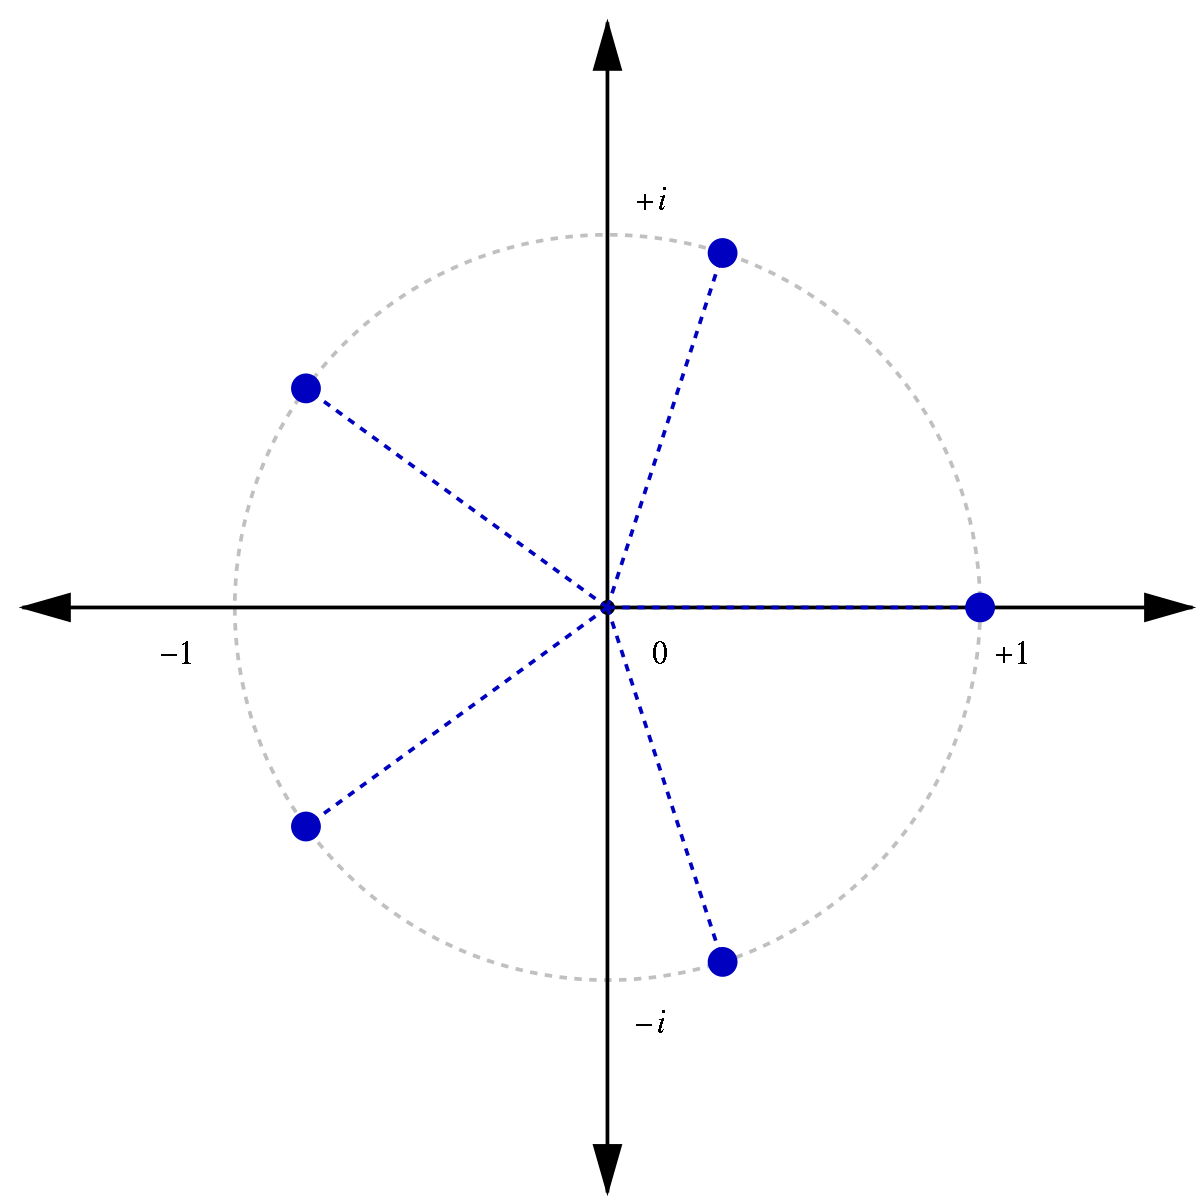
\includegraphics[scale=0.19]{Images/1200px-One5Root.svg.png}
    \caption{Fifth roots of unity}
\end{figure}
\end{example}
In order to finish our characterization of cyclic extensions we need the following lemma.
\begin{lemma}\em
Let $n$ be a positive integer and $K$ a field which contains a primitive $n$-th root of unity $\zeta$.\par
(i) If $d\mid n$, then $\zeta^{n/d}=\eta$ is a primitive $d$-th root of unity in $K$.\par
(ii) If $d\mid n$ and $u$ is a nonzero root of $x^d-a\in K[x]$, then $x^d-a$ has $d$ distinct roots, namely $u$, $\eta u$, $\cdots$, $\eta^{d-1}u$, where $\eta\in K$ is a primitive $d$-th root of unity. Furthermore $K(u)$ is a splitting field of $x^d-a$ over $K$ and is Galois over $K$.
\end{lemma}
\begin{proof}
(i) Suppose $d\mid n$, note that $\eta^d=(\zeta^{n/d})^d=\zeta^n=1_K$, therefore $\eta$ is the $d$-th primitive root of unity.\par
(ii) We first show that $\eta^iu$ is a root of the polynomial $x^d-a\in K[x]$. Note that 
$$
\left( \eta ^iu \right) ^d=\eta ^{id}u^d=\left( \eta ^d \right) ^iu^d=1_{K}^{i}u^d=u^d=a,
$$
whence $u,\eta u,\cdots,\eta^{n-1}u$ are distinct roots of the polynomial $x^d-a$. Now suppose $F=K(u)$, trivially $K(\eta^iu)=K(u)$ since $\zeta\in K$, therefore $K(u)$ is a splitting field of $x^d-a$ over $K$. Note also $F/K$ is separable, we therefore conclude that $F/K$ is a Galois extension.
\end{proof}
\begin{theorem}
Let $n$ be a positive integer and $K$ a field which contains a primitive $n$-th root of unity $\zeta$. Then the following statements are equivalent: \par
(i) $F$ is cyclic over $K$ of degree $d\mid n$;\par
(ii) $F$ is a splitting field over $K$ of a polynomial of the form $x^n-a\in K[x]$. Under which circumstances we have $F=K(u)$, where $u$ is a root of $x^n-a$;\par
(iii) $F$ is a splitting field over $K$ of an irreducible polynomial $x^d-b\in K[x]$. Under which circumstances we have $F=K(v)$, where $v$ is a root of $x^d-b$.
\end{theorem}
\begin{proof}
(ii)$\Rightarrow$(i): Suppose $F$ is a splitting field over $K$ of a polynomial of the form $x^n-a\in K[x]$. By Lemma 6.20 we have $F=K(u)$, where $u$ is a root of $x^n-a$, and $F/K$ is a Galois extension. Now suppose $\sigma\in\mathrm{Gal}(F/K)$, then $\sigma$ is completely determined by $\sigma(u)=\zeta^iu$, where $\zeta$ is the primitive $n$-th unit root. Therefore we may define a homomorphism $\theta:\mathrm{Gal}(F/K)\to\mathbb{Z}_n$ given by $\sigma\mapsto\zeta^i$ provided $\sigma(u)=\zeta^iu$. It is routine to verify $\theta$ is well-defined and a monomorphism. Therefore $\mathrm{Gal}(F/K)$ is a subgroup of $\mathbb{Z}_n$, whence a cyclic group of order $d\mid n$.\par
(i)$\Rightarrow$(iii): Suppose $F$ is cyclic over $K$ of degree $d\mid n$. Then $\mathrm{Gal}(F/K)$ is cyclic. Suppose $\mathrm{Gal}(F/K)=\left<\sigma\right>$. Let $\eta=\zeta^{n/d}$ be the primitive $d$-th root of unity. Note that 
$$
N_{K}^{F}\left( \eta \right) =\eta ^{\left[ F:K \right]}=\left( \zeta ^{n/d} \right) ^d=\zeta ^n=1_K,
$$
we therefore by Hilbert 90 to conclude that there exists some $w\in F$ such that $\eta=w\sigma(w)^{-1}$. Suppose $v=w^{-1}$, we claim that $v^d\in K$. To see this, note that 
$$
\sigma \left( v^d \right) =\sigma \left( v \right) ^d=\left( \eta v \right) ^d=\eta ^dv^d=1_Kv^d=v^d,
$$
whence $v^d$ is fixed by $\sigma$ and hence in $K$. Now suppose $b=v^d$, we have $v$ a root of $x^d-b\in K[x]$, and $K(v)$ is a splitting field over $K$ of $x^d-b$. We further show that $x^d-b$ is irreducible. Consider $\sigma^i:K(u)\to K(\eta^iu)$. Since $\eta^i\in K$, we have $K(u)\cong K(\eta^iu)$ for all $i\in\mathbb{Z}_d$ and hence $x^d-b$ is irreducible. Now it suffices to show that $F=K(v)$. To see this, note that $[K(v):K]=[F:K]=d$, hence $K(v)=F$.\par
(iii)$\Rightarrow$(ii): If $v\in F$ is a root of $x^d-b\in K[x]$, then $F=K(v)$ by Lemma 6.20. Now note that 
$$
\left( \zeta v \right) ^n=\zeta ^nv^n=1_Kv^{d\left( n/d \right)}=b^{n/d}\in K,
$$
therefore $\zeta v$ is a root of $x^n-a\in K[x]$, where $a=b^{n/d}$. By Lemma 6.20 we have $F=K(\zeta v)$ a splitting field of $x^n-a\in K[x]$. However $F=K(v)=K(\zeta v)$ since $\zeta\in K$, which finished the proof.
\end{proof}
It is clear that the primitive $n$-th root of unity plays an important role in the proof of the preceding results. Characterization of the splitting fields of polynomials of the form $x^n-a\in K[x]$ is considerably more difficult when $K$ does not contain a primitive $n$-th root of unity. The case when $a=1_K$ is considered in the next section.
\begin{center}
\begin{large}
    \textbf{Exercises for 6.7}
\end{large}
\end{center}
\begin{problem}\em
If $\overline{K}$ is replaced by any normal extension $N$ of $K$ containing $F$, then this new definition of norm and trace is equivalent to the original one. In particular, the new definition does not depend on the choice of $N$.
\end{problem}
\begin{proof}
Note that if $\overline{K}$ is substituted with $N$, a homomorphism $\sigma:K\to N$ must be a homomorphism $\sigma:K\to\overline{K}$. Therefore it suffices to show that the number of different homomorphisms of $K\to\overline{K}$ and $K\to N$ are the same. Since $\overline{K}$ is normal over $K$ and $\overline{K}\supset F$, then the number of different $\sigma:F\to\overline{K}$ equals to $[F:K]_s$. Similarly we have number of different $\sigma:F\to N$, where $N$ is a normal extension field over $K$ that contains $F$, equals to $[F:K]_s$. Therefore two definitions are equivalent.
\end{proof}
\begin{problem}\em
Let $F$ be a finite dimensional extension of a finite field $K$. The norm ${N_K}^F$ and the trace ${T_K}^F$ (considered as maps $F\to K$) are surjective.
\end{problem}
\begin{proof}
We shall first consider the trace condition. Note that $T_K^F$ is a linear functional, therefore it is either trivial or surjective. Note that if $F$ is a finite dimensional extension of a finite field $K$, then $F/K$ is separable and hence 
$$
T_{K}^{F}\left( u \right) =\left[ F:K \right] _i\cdot \sum_{i=1}^n{\sigma _i\left( u \right)},\hspace{0.5cm}u\in F
$$
is nontrivial, therefore $T_K^F$ is surjective. Note also $N_K^F$ is a linear functional with respect to multiplication, we finished the proof.
\end{proof}
\begin{problem}\em
Let $\overline{\mathbb{Q}}$ be a (fixed) algebraic closure of $\mathbb{Q}$ and $v\in \overline{\mathbb{Q}}, v\notin \mathbb{Q}$. Let $E$ be a subfield of $\overline{\mathbb{Q}}$ maximal with respect to the condition $v\notin E$. Prove that every finite dimensional extension of $E$ is cyclic.
\end{problem}
\begin{proof}
Let $F$ be an extension field of $E$ of finite dimension. We may suppose $F$ is a normal extension field of $E$, or otherwise take the normal closure of $F$ in $E$. Now by definition of $E$ we have $F\supset E(v)$. If $\mathrm{Gal}(F/E)=G$, and the group fixing $E(v)$ is $H$, then $H\subset G$, and any proper subgroup of $G$ is contained in $H$, since for any $E\subset L\subset F$, $L\ne E$, we have $L\supset E(v)$. Therefore if $g\in G$, $g\notin H$, we have the cyclic group $\left<g\right>$ must equal to $G$, hence $G$ is cyclic. This finished the proof.
\end{proof}
\begin{problem}\em
Let $K$ be a field,
$\overline{K}$ an algebraic closure of $K$ and $\sigma\in \mathrm{Gal}(\overline{K}/K)$. Let 
$$F=\{u\in \overline{K}: \sigma(u)=u\}.$$
Then $F$ is a field and every finite dimensional extension of $F$ is cyclic.
\end{problem}
\begin{proof}
$F$ is trivially a field. We now show that if $E/F$ finite dimensional, then $E/F$ is cyclic. Suppose $N/F$ is a normal extension such that $[N:F]<\infty$. It suffices to show that $N/F$ is cyclic. Take $\sigma\in G=\mathrm{Gal}(N/F)$, and let $H=\left<\sigma\right>$ a subgroup of $G$. We now show that $H=G$. Let $N^H$ be the fixed field of $H$, therefore if $x\in H$, then $x$ is fixed by elements in $H$, whence fixed by $\sigma$, hence $x\in F$. Therefore $[N^H:F]=1$, which implies $[G:H]=1$ and hence $G=H$ is cyclic.
\end{proof}
\begin{problem}\em
If $F$ is a cyclic extension of $K$ of degree $p^n$ ($p$ prime) and $L$ is an intermediate field such that $F=L(u)$ and $L$ is cyclic over $K$ of degree $p^{n-1}$, then $F=K(u)$.
\end{problem}
\begin{proof}
Suppose $\mathrm{Gal}(F/K)=\left<\sigma\right>\cong\mathbb{Z}_{p^n}$. Therefore we have $\mathrm{Gal}(F/L)=\left<\sigma^{p^{n-1}}\right>$. Now suppose $\sigma^{p^i}\in\mathrm{Gal}(F/K(u))$, then $\sigma^{p^i}(u)=u$, and hence the only possibility would be $i=n$, which implies $\mathrm{Gal}(F/K(u))$ is trivial. Therefore $F=K(u)$.
\end{proof}
\begin{problem}\em
If $\mathrm{char}F=p\neq 0$, let $K_p=\{u^p-u: u\in K\}$.\par
(i) A cyclic extension field $F$ of $K$ of degree $p$ exists if and only if $K\neq K_p$.\par
(ii) If there exists a cyclic extension of degree $p$ of $K$, then there exists a cyclic extension of degree $p^n$ for every $n\geq 1$.
\end{problem}
\begin{proof}
(i) Suppose there exists an extension field $F$ of $K$ of degree $p$, we prove by contradiction. Suppose $K_p=K$, then $F$ is the splitting field over $K$ of the irreducible polynomial $x^p-x-a\in K[x]$. However since $a\in K$, there exists some $u\in K$ such that $u^p-u=a$, which implies $u$ is a root of $x^p-x-a\in K[x]$, whence the polynomial is not irreducible, a contradiction! Conversely, suppose $K=K_p$, then every polynomial of the form $x^p-x-a\in K[x]$ splits in $K$, whence the only splitting field of $x^p-x-a$ over $K$ are trivial. Hence there are no cyclic extensions of degree $p$ of $K$.\par
(ii) We proof by induction. Suppose $n=1$, then the proposition is trivial. Now if $n>1$, suppose $E/K$ is a cyclic extension of degree $p^{n-1}$ with $\mathrm{Gal}(E/K)=\left<\sigma\right>\cong\mathbb{Z}_{p^{n-1}}$. Now take $z\in E$ such that $T_K^E(z)\ne 0$, define $v=T_K^E(z)^{-1}z$, we have $T_K^E(v)=1_K$ and $v\in E$. Therefore by Hilbert 90 there exists some $u\in E$ such that $\sigma(u)-u=v^p-v$. Now $x^p-x-u\in E[x]$ is irreducible and suppose $w$ is a root of $x^p-x-u$, we have $K(w)$ a desired extension field.
\end{proof}
\begin{problem}\em
If $n$ is an odd integer such that $K$ contains a primitive $n$th root of unity and $\mathrm{char}K\neq 2$, then $K$ also contains a primitive $2n$th root of unity.
\end{problem}
\begin{proof}
Let $\zeta$ be the primitive $n$-th root of unity in $K$. Then consider $-\zeta^2$, which generates a cyclic group of order $2n$ since 
$$
\left( -\zeta ^2 \right) ^{2n}=\left( -1 \right) ^{2n}\left( \zeta ^2 \right) ^{2n}=\zeta ^{4n}=\left( \zeta ^n \right) ^4=1_K,
$$
which finished the proof.
\end{proof}
\begin{problem}\em
Which roots of unity are contained in the following fields: $\mathbb{Q}(\mathrm{i})$, $\mathbb{Q}(\sqrt{2})$, $\mathbb{Q}(\sqrt{3})$, $\mathbb{Q}(\sqrt{5})$, $\mathbb{Q}(\sqrt{-2})$, $\mathbb{Q}(\sqrt{-3})$?
\end{problem}
\begin{proof}
We shall denote $\zeta_n$ the primitive $n$-th root of unity. Note first $\mathbb{Q}(\mathrm{i})$ contains $\zeta_2$ and $\zeta_4$, and $\mathbb{Q}(\sqrt{2})$, $\mathbb{Q}(\sqrt{3})$, $\mathbb{Q}(\sqrt{5})$, as subspaces of $\mathbb{R}$, contains $\zeta_2$. Now we analyze $\mathbb{Q}(\sqrt{-2})$ and $\mathbb{Q}(\sqrt{-3})$. Note first $\mathbb{Q}(\zeta_n)/\mathbb{Q}$ is a cyclic extension field of order $\varphi(n)$, where $\varphi(n)$ is the Euler totient function, and $[\mathbb{Q}(\sqrt{-3}):\mathbb{Q}]=[\mathbb{Q}(\sqrt{-2}):\mathbb{Q}]=2$, we have $\varphi(n)=2$ and hence $n=2,3,4,6$. Note 
$$
\zeta _2=-1,\hspace{0.5cm}\zeta _3=-\frac{1}{2}-\frac{\sqrt{3}}{2}\mathrm{i},\hspace{0.5cm}\zeta _4=\mathrm{i},\hspace{0.5cm}\zeta _6=\frac{1}{2}+\frac{\sqrt{3}}{2}\mathrm{i},
$$
we have $\mathbb{Q}(\sqrt{-2})$ contains $\zeta_2$ and $\mathbb{Q}(\sqrt{-3})$ contains $\zeta_2$, $\zeta_3$ and $\zeta_6$.
\end{proof}
\subsection{Cyclotomic Extensions}
We shall examine splitting fields of the polynomial $x^n-1_K$ in this section, with special attention to the case $K=\mathbb{Q}$.\par
A splitting field $F$ over a field $K$ of $x^n-1_K\in K[x]$ (where $n\ge 1$) is called a \textbf{cyclotomic extension} of order $n$. If $\mathrm{char}K=p\ne 0$ and $n=mp^t$ with $(p,m)=1$, then $x^n-1_K=(x^m-1_K)^{p^t}$ and hence the cyclotomic extension of order $n$ coincides with the one of order $m$. Thus we shall usually assume that $\mathrm{char}K$ does not divide $n$, i.e. $\mathrm{char}K=0$ or $\mathrm{char}K$ is relatively prime to $n$.\par
The dimension of a cyclotomic extension field of order $n$ is related to the \textbf{Euler function} $\varphi(n)$ of elementary number theory, which assigns to each positive integer $n$ the number $\varphi(n)$ of integers $i$ such that $1\le i\le n$ and $(i,n)=1$. For example, $\varphi(6)=2$ and $\varphi(p)=p-1$ provided $p$ is a prime.
\begin{theorem}
Let $n$ be a positive integer, $K$ a field such that $\mathrm{char}K$ does not divide $n$ and $F$ a cyclotomic extension of $K$ of order $n$.\par
(i) $F=K(\zeta)$, where $\zeta\in F$ is a primitive $n$-th root of unity;\par
(ii) $F$ is an abelian extension of dimension $d$, i.e. the $F$ is an algebraic Galois extension of $K$ with $\mathrm{Gal}(F/K)$ abelian, and $d\mid \varphi(n)$, here $\varphi(n)$ is the Euler function. If $n$ is a prime then $F/K$ is a cyclic extension.\par
(iii) $\mathrm{Gal}(F/K)$ is isomorphic to a subgroup of order $d$ of the multiplicative group of units $\mathbb{Z}_n$.
\end{theorem}
\begin{proof}
(i) Note that $F$ contains a primitive $n$-th root of unity $\zeta$. By definition $1_K$, $\zeta$, $\cdots$, $\zeta^{n-1}\in K(\zeta)$ are the $n$ roots of the polynomial $x^n-1_K\in K[x]$, whence $F=K(\zeta)$.\par
(ii) Trivially the polynomial $x^n-1_K$ is separable over $K$, hence $F/K$ is a Galois extension. Suppose $\sigma\in\mathrm{Gal}(F/K)$, then $\sigma$ is completely determined by $\sigma(\zeta)$. For some $i$, we have $\sigma(\zeta)=\zeta^i$ and for some $j$ we have $\sigma^{-1}(\zeta)=\zeta^j$, whence $\zeta=\sigma^{-1}\sigma(\zeta)=\zeta^{ij}$, hence $ij\equiv 1\pmod{n}$. Note that this implies $i$ a unit in $\mathbb{Z}_n$. Consider the homomorphism $\mathrm{Gal}(F/K)\to G$ given by $\sigma\mapsto\overline{\iota}$, where $\overline{\iota}$ is the image of $i$ such that $\sigma(\zeta)=\zeta^i$ in $G$ and $G$ is the multiplicative subgroup of $\mathbb{Z}_n$ consists of all units in $\mathbb{Z}_n$. It is routine to show that the homomorphism is well-defined and a monomorphism. Therefore $\mathrm{Gal}(F/K)\cong\mathrm{Im}f$ is abelian with order $d$ dividing $\varphi(n)$, since $|G|=\varphi(n)$.\par
(iii) has already been proved in (ii). Note that if $n$ is a prime, then $\mathbb{Z}_n$ is a field, and hence $\mathrm{Gal}(F/K)$ is cyclic by Theorem 6.54.
\end{proof}
Let $n$ be a positive integer, $K$ a field such that $\mathrm{char}K$ does not divide $n$, and $F$ a cyclotomic extension of order $n$ of $K$. The \textbf{$n$-th cyclotomic polynomial} over $K$ is the monic polynomial $\Phi_n(x)=(x-\zeta_1)(x-\zeta_2)\cdots(x-\zeta_r)$, where $\zeta_r$ are distinct primitive $n$-th roots of unity in $F$.
\begin{example}\em
It is easily computed some cyclotomic polynomials when $n$ is small. For instance, we have $\Phi_1(x)=x-1_K$, $\Phi_2(x)=(x-(-1_K))=x+1_K$. If $K=\mathbb{Q}$, then we have 
$$
\Phi _3\left( x \right) =\left( x-\left( -\frac{1}{2}+\frac{\sqrt{3}}{2}\mathrm{i} \right) \right) \left( x-\left( -\frac{1}{2}-\frac{\sqrt{3}}{2}\mathrm{i} \right) \right) =x^2+x+1
$$
and 
$$
\Phi _4\left( x \right) =\left( x-\mathrm{i} \right) \left( x+\mathrm{i} \right) =x^2+1.
$$
\end{example}
These examples suggests the following properties of cyclotomic polynomials.
\begin{proposition}
Let $n$ be a positive integer, $K$ a field such that $\mathrm{char}K$ does not divide $n$ and $\Phi_n(x)$ the $n$-th cyclotomic polynomial of $K$.\par
(i) $x^n-1_K=\prod_{d\mid n}\Phi_d(x)$;\par
(ii) The coefficients of $\Phi_n(x)$ lie in the prime subfield $P$ of $K$. If $\mathrm{char}K=0$ and $P$ is identified with the field $\mathbb{Q}$ of rationals, then the coefficients are actually integers.\par
(iii) $\mathrm{deg}\Phi_n(x)=\varphi(n)$, where $\varphi$ is the Euler function.
\end{proposition}
\begin{proof}
(i) Suppose $F/K$ is a cyclotomic extension of order $n$, then $\mathrm{Gal}(F/K)=\left<\zeta\right>$ and hence 
$$
x^n-1_K=\prod_{\eta \in \mathrm{Gal}\left( F/K \right)}{\left( x-\eta \right)}=\prod_{d\mid n}{\prod_{\substack{\eta \in \mathrm{Gal}\left( F/K \right) \\ \left| \eta \right|=d}}{\left( x-\eta \right)}}=\prod_{d\mid n}{\Phi _d\left( x \right)},
$$
which finished the proof.\par
(ii) We proof by induction. For $n=1$, we have $\Phi_1(x)=x-1_K$ and the statement is trivial. Now suppose the statement is true for all $k<n$. Define $f(x)=\prod_{\substack{d\mid n \\ d<n}}\Phi_d(x)$, we therefore have $x^n-1_K=f(x)\Phi_n(x)$ by (i). On the other hand $f(x)$ is monic, and $f\in P[x]$. By the division algorithm over $P[x]$ we have $x^n-1_K=f(x)k(x)+r(x)$, where $k,r\in P[x]\subset F[x]$. However by the uniqueness of division algorithm (over $F[x]$) we must have $r=0$ and $k=\Phi_n$, whence $\Phi_n=k\in P[x]$, which finished the proof. For $K=\mathbb{Q}$, the proof is analogous with $P$ replaced by $\mathbb{Z}$.\par
(iii) Trivially $\mathrm{deg}\Phi_n$ equals to the number of distinct primitive $n$-th roots of unity. Note that if $\zeta$ is a primitive $n$-th root of unity, then $\zeta^k$ is also a primitive $n$-th root of unity if and only if $(k,n)=1$, hence $\mathrm{deg}\Phi_n$ equals to the number of elements in $\{k\in\mathbb{Z}:(k,n)=1\}$, which is precisely $\varphi(n)$.
\end{proof}
\begin{note}\em
Proposition 6.83 offered a recursive method to determine the cyclotomic polynomials. Suppose we would like to calculate $\Phi_6$ over $\mathbb{Q}$. Then since we have already known $\Phi_1$, $\Phi_2$ and $\Phi_3$, we have 
$$
\Phi _6\left( x \right) =\frac{x^n-1}{\prod_{\substack{d\mid n \\ d<n}}{\Phi _d\left( x \right)}}=\frac{x^6-1}{\left( x-1 \right) \left( x+1 \right) \left( x^2+x+1 \right)}=x^2-x+1.
$$
Furthermore, we have 
$$
\Phi _{12}\left( x \right) =\frac{x^{12}-1}{\Phi _1\left( x \right) \Phi _2\left( x \right) \Phi _3\left( x \right) \Phi _6\left( x \right)}=x^4-x^2+1.
$$
\end{note}
We now investigate the cyclotomic polynomials over $\mathbb{Q}$.
\begin{proposition}
Suppose $F$ is a cyclotomic extension field of $\mathbb{Q}$ and $\Phi_n$ the $n$-th cyclotomic polynomial over $\mathbb{Q}$.\par
(i) $\Phi_n(x)$ is irreducible over $\mathbb{Q}[x]$.\par
(ii) $[F:\mathbb{Q}]=\varphi(n)$, where $\varphi$ is the Euler function.\par
(iii) $\mathrm{Gal}(F/\mathbb{Q})$ is isomorphic to the multiplicative group of units in $\mathbb{Z}_n$.
\end{proposition}
\begin{proof}
(i) It suffices to show that $\Phi_n(x)$ is an irreducible monic polynomial over $\mathbb{Z}[x]$. Suppose $h(x)$ is an irreducible factor of $\Phi_n(x)$ over $\mathbb{Z}$, then there exists some $f\in\mathbb{Z}[x]$ such that $\Phi_n(x)=f(x)h(x)$. Suppose $\mathrm{deg}f\ge 1$. Let $\zeta$ be a root of $h$ and $p$ a prime number such that $(p,n)=1$. Since $h$ is an irreducible factor of $\Phi_n$, we have $\zeta$ a primitive $n$-th root of unity. We now claim that $\zeta^p$ is also a root of $h$. Since $\zeta^p$ is also a primitive $n$-th root of unity by $(p,n)=1$, we have $\zeta^p$ either a root of $h$ or a root of $f$. Suppose $\zeta^p$ is a root of $f$, then $\zeta$ is a root of $f(x^p)$. Since $h(x)$ is irreducible over $\mathbb{Q}[x]$, we have $h(x)\mid f(x^p)$ and hence $f(x^p)=h(x)k(x)$ for some $k(x)\in\mathbb{Q}[x]$. Consider the division algorithm in $\mathbb{Z}[x]$ which states $f(x^p)=h(x)k_1(x)+r(x)$, we therefore have $k_1(x)=k(x)\in\mathbb{Z}[x]$. Now we $\bmod{p}$ on both side of $f(x^p)=h(x)k(x)$ and obtain $\overline{f}(x^p)=\overline{f}(x)^p=\overline{h}(x)\overline{k}(x)$, with $\overline{f}\equiv f\pmod{p}$. Now suppose $\overline{l}(x)$ is a irreducible factor of $\overline{h}(x)$, then $\mathrm{l}(x)\mid \overline{f}(x)^p$, whence $\mathrm{l}\mid\overline{f}$ by the unique factorization over $\mathbb{Z}_p[x]$. Now note that $x^n-1_K=\Phi_n(x)m(x)=f(x)h(x)m(x)$, we therefore by $\bmod{p}$ have 
$$
x^n-\overline{1_K}=\overline{x^n-1_K}=\overline{f}\left( x \right) \overline{h}\left( x \right) \overline{m}\left( x \right) .
$$
Note that $\overline{h}(x)$ and $\overline{f}(x)$ have a common divisor $\overline{l}(x)$, which states that $\overline{x^n-1_K}$ has a multiplicative root, a contradiction! Therefore $\zeta^p$ is a root of $h(x)$. Now suppose $r\in\mathbb{Z}$ with $(r,n)=1$, then suppose $r=p_1^{k_1}p_2^{k_2}\cdots p_s^{k_s}$ with $p_i$ prime and $k_i\in\mathbb{Z}_+$, then $(p_i,n)=1$ and hence, using the preceding result repeatedly, $\zeta^r$ is a root of $h$. However this implies $\prod_{\substack{1\le r\le n \\ r\mid n}}(x-\zeta^r)=\Phi_n(x)$ divides $h(x)$, which implies $\Phi_n(x)=h(x)$ and the proof is finished.\par
(ii) Note that 
$$
\left[ F:\mathbb{Q} \right] =\left[ \mathbb{Q} \left( \zeta \right) :\mathbb{Q} \right] =\mathrm{deg}\Phi _n=\varphi \left( n \right) .
$$\par
(iii) Since the multiplicative group of units in $\mathbb{Z}_n$ is of order $\varphi(n)$, and $|\mathrm{Gal}(F/\mathbb{Q})|=\varphi(n)$, we therefore have $\mathrm{Gal}(F/\mathbb{Q})$ is isomorphic to the multiplicative group of units in $\mathbb{Z}_n$.
\end{proof}
A nontrivial theorem of Kronecker states that every abelian extension of $\mathbb{Q}$ is contained in a cyclotomic extension, which we only mention but not proof this result here.
\begin{center}
\begin{large}
    \textbf{Exercises for 6.8}
\end{large}
\end{center}
\begin{problem}\em
If $i\in \mathbb{Z}$, let $\overline{i}$ denote the image of $i$ in $\mathbb{Z}_n$ under the canonical projection $\mathbb{Z}\to \mathbb{Z}_n$. Prove that $\overline{i}$ is a unit in the ring $\mathbb{Z}_n$ if and only if $\gcd{(i, n)}=1$. Therefore the multiplicative group of units in $\mathbb{Z}_n$ has order $\varphi(n)$.
\end{problem}
\begin{proof}
It suffices to proof that $(i,n)=1$ if and only if there exists some $j\in\mathbb{Z}$ such that $ij\equiv 1\pmod{n}$. Suppose $(i,n)=1$, then there exists some integers $j,h\in\mathbb{Z}$ such that $ij+hn=1$, hence $ij=-hn+1\equiv 1\pmod{n}$. Conversely, suppose there exists some $j\in\mathbb{Z}$ such that $ij\equiv 1\pmod{n}$, then $ij-1=kn$ for some $k\in\mathbb{Z}$. Suppose $\gcd(i,n)=d$, then $d\mid i$ and $d\mid n$, whence $d\mid ij-kn=1$, hence $d=1$.
\end{proof}
\begin{problem}\em
Establish the following properties of the Euler function $\varphi$.\par
(a) If $p$ is prime and $n>0$, then $\varphi(p^n)=p^n(1-1/p)=p^{n-1}(p-1)$.\par
(b) If $\gcd{(m, n)}=1$, then $\varphi(mn)=\varphi(m)\varphi(n)$.\par
(c) If $n=p_1^{k_1}\cdots p_r^{k_r}$ ($p_i$ distinct primes; $k_i>0$), then $\varphi(n)=n(1-1/p_1)(1-1/p_2)\cdots (1-1/p_r)$.\par
(d) $\sum_{d\mid n}\varphi(d)=n$.\par
(e) $\varphi(n)=\sum_{d\mid n}d\mu(n/d)$, where $\mu$ is the Moebius function defined by
$$
\mu(n)=
\left\{\begin{array}{ll}
1 & \text{if }n=1 \\
(-1)^t & \text{if }n \text{ is a product of }t\text{ distinct primes}\\
0 & \text{if }p^2\text{ divides }n\text{ for some prime }p.
\end{array}\right.
$$
\end{problem}
\begin{proof}
Our proof is due to Apostol: \textit{Introduction to Analytic Number Theory}.\par
(a) Trivially $\varphi(p)=p-1$. Now for $n>1$, the only possible divisor of $p^n$ are $p, 2p,\cdots, p^2, (p+1)p,\cdots, p^n$, whence $\varphi(p^n)=p^n-p^{n-1}=p^{n-1}(p-1)$.\par
(e) We first show that $\sum_{d\mid n}\mu(d)=\lfloor 1/n \rfloor$. The condition $n=1$ is trivial. Now if $n>1$, suppose $n=p_1^{\alpha_1}p_2^{\alpha_2}\cdots p_k^{\alpha_k}$. Then 
$$
\begin{aligned}
\sum_{d\mid n}{\mu \left( d \right)}&=1+\mu \left( p_1 \right) +\cdots +\mu \left( p_n \right) -\mu \left( p_1p_2 \right) -\cdots -\mu \left( p_{k-1}p_k \right) +\cdots +\frac{\left( -1 \right) ^k}{p_1p_2\cdots p_k}
\\
&=1+C_{k}^{1}\left( -1 \right) +C_{k}^{2}\left( -1 \right) ^2+\cdots +C_{k}^{k}\left( -1 \right) ^k=\left( 1-1 \right) ^k=0,
\end{aligned}
$$
which finished the proof. Now we show $\varphi(n)=\sum_{d\mid n}d\mu(n/d)$. Indeed we have 
$$
\varphi \left( n \right) =\sum_{k=1}^n{\left\lfloor \frac{1}{\left( n,k \right)} \right\rfloor}=\sum_{k=1}^n{\sum_{d\mid \left( n,k \right)}{\mu \left( d \right)}}=\sum_{k=1}^n\sum_{\substack{d\mid n \\ d\mid k}}\mu(d)=\sum_{d\mid n}{\sum_{q=1}^{n/d}{\mu \left( d \right)}}=\sum_{d\mid n}{\frac{n}{d}\mu \left( d \right)},
$$
which finished the proof.\par
(d) Denote $S=\{1,2,\cdots,n\}$. Suppose $A(d)=\{k\in S:(k,n)=d\}$, then $\{A(d)\}_{d\mid n}$ forms a partition of $S$ and hence if we denote the number of elements in $A(d)$ as $f(d)$, we have $\sum_{d\mid n}f(d)=n$. However $(k,n)=d$ if and only if $(k/d,n/d)=1$, whence 
$$
\sum_{d\mid n}{\varphi \left( d \right)}=\sum_{d\mid n}{\varphi \left( \frac{n}{d} \right)}=\sum_{d\mid n}{f\left( d \right)}=n.
$$\par
(c) Note that if $n=p_1^{\alpha_1}p_2^{\alpha_2}\cdots p_k^{\alpha_k}$, then 
$$
\prod_{p\mid n}{\left( 1-\frac{1}{p} \right)}=\prod_{i=1}^k{\left( 1-\frac{1}{p_i} \right)}=1-\sum_i{\frac{1}{p_i}}+\sum_{i,j}{\frac{1}{p_ip_j}}-\cdots +\frac{\left( -1 \right) ^k}{p_1p_2\cdots p_k}=\sum_{d\mid n}{\frac{\mu \left( d \right)}{d}},
$$
combined with (e) to finish the proof.\par
(b) Note that by (c) we have 
$$
\frac{\varphi \left( mn \right)}{mn}=\frac{\prod_{p\mid m}{\left( 1-\frac{1}{p} \right)}\prod_{p\mid n}{\left( 1-\frac{1}{p} \right)}}{\prod_{p\mid \left( m,n \right)}{\left( 1-\frac{1}{p} \right)}}=\prod_{p\mid m}{\left( 1-\frac{1}{p} \right)}\prod_{p\mid n}{\left( 1-\frac{1}{p} \right)}=\frac{\varphi \left( m \right)}{m}\cdot \frac{\varphi \left( n \right)}{n},
$$
hence $\varphi(mn)=\varphi(m)\varphi(n)$.
\end{proof}
\begin{problem}\em
Let $\varphi$ be the Euler function.\par
(a) $\varphi(n)$ is even for $n>2$.\par
(b) Find all $n>0$ such that $\varphi(n)=2$.\par
(c) Find all pairs $(n, p)$ (where $n, p>0$, and $p$ is prime) such that $\varphi(n)=n/p$.
\end{problem}
\begin{proof}
(a) Suppose $n>2$, then apart from numbers of the form $2^m$ there exists an odd prime $p$ divides $n$. Suppose $n=2^m$. Since $2$ is a prime, we have $\varphi(2^m)=2^m-2^{m-1}=2^{m-1}$, which is even since $m\ge 2$. Otherwise there exists a prime $p\mid n$ and hence 
$$
\varphi \left( n \right) =n\prod_{p\mid n}{\left( 1-\frac{1}{p} \right)}=\frac{n\left( p-1 \right)}{p}\prod_{\substack{q\mid n \\ q\ne p}}\left( 1-\frac{1}{q} \right),
$$
which is divisible by $p-1$, and hence by $2$. Therefore $\varphi(n)$ is even for $n>2$.\par
(b) Note that 
$$
\varphi \left( n \right) =n\prod_{p\mid n}{\left( 1-\frac{1}{p} \right)}\ge \prod_{p\mid n}{p\left( 1-\frac{1}{p} \right)}=\prod_{p\mid n}{\left( p-1 \right)},
$$
therefore if $n>6$, we have $\varphi(n)>2$ and hence the only possible candidate for the solution are $n\le 6$. Verify one by one to obtain the solution of $\varphi(n)=2$ being $n=3,4$ and $6$.\par
(c) Pending...
\end{proof}
\begin{problem}\em
(a) If $p$ is an odd prime and $n>0$, then the multiplicative group of units in the ring $\mathbb{Z}_{p^n}$ is cyclic of order $p^{n-1}(p-1)$.\par
(b) Part (a) is also true if $p=2$ and $1\leq n\leq 2$.\par
(c) If $n\geq 3$, then the multiplicative group of units in $\mathbb{Z}_{2^n}$ is isomorphic to $\mathbb{Z}_2\oplus \mathbb{Z}_{2^{n-2}}$.
\end{problem}
\begin{proof}
(a) Denote the multiplicative group of units in the ring $\mathbb{Z}_{p^n}$ as $\mathbb{Z}_{p^n}^\times$. Then by Exercise 6.90 we have $|\mathbb{Z}_{p^n}^\times|=\varphi(p^n)=p^{n-1}(p-1)$. Now it suffices to show that $\mathbb{Z}_{p^n}^\times$ is cyclic. We break the proof into several steps.\par
We first show the following conclusion: Suppose $G$ is an abelian group, $a,b\in G$ with $|a|=m$, $|b|=n$, then there exists some elements $c\in G$ such that $|c|=[m,n]$ (the least common divisor of $m$ and $n$). To show this, note first if $k\mid n$ with $a$ of order $n$, then there exists some elements, for instance, $a^{n/d}$, has order $k$. Therefore we have elements of order $(m,n)$, $m/(m,n)$ and $n/(m,n)$, and note that if $a$ is of order $m$ and $b$ is of order $n$, then $ab$ is of order $mn$, we have shown that there exists some elements in $G$ of order $[m,n]$. Similarly we may extend this result to the condition of finding an element of order of the least common divisor of finitely many elements.\par
We now show that if $d\mid p-1$, where $p$ is a prime, then the polynomial $x^d-1$ has exactly $d$ distinct roots in $\mathbb{Z}_p^\times$. To see this, note first if $d\mid p-1$, then there exists some $d^\prime\in\mathbb{Z}$ such that $dd^\prime=p-1$. Therefore we have 
$$
\frac{x^{p-1}-1}{x^d-1}=\frac{\left( x^d \right) ^{d^{\prime}}-1}{x^d-1}=\sum_{k=1}^{d^{\prime}}{\left( x^d \right) ^{k-1}}=g\left( x \right) ,
$$
and hence $x^{p-1}-1=(x^d-1)g(x)$. Now we $\bmod{p}$ on both side, suppose $x^d-\overline{1}$ has less than $d$ roots in $\mathbb{Z}_p^\times$, then since $\mathrm{deg}g=dd^\prime-d$, we have the number of roots in $x^{p-1}-\overline{1}$ is less than $p-1$, a contradiction! Therefore there are precisely $d$ roots of $x^d-1$ in $\mathbb{Z}_p^\times$.\par
Now we show that $\mathbb{Z}_p^\times$ is cyclic. Suppose not. Then suppose $i\in\mathbb{Z}_p^\times$, we denote $|i|=m_i$. Let $d=[m_1,\cdots,m_{p-1}]$, by the preceding results we know that there exists some $g\in\mathbb{Z}_p^\times$ such that $|g|=d$. Now consider the polynomial $x^d-1$, it has only $d$ roots in $\mathbb{Z}_p^\times$. However if $i\in\mathbb{Z}_p^\times$, then $|i|=m_i\mid d$ and hence 
$$
i^d-1=\left( i^{m_i} \right) ^{d/m_i}-1=1^{d/m_i}-1=0,
$$
which implies every element in $\mathbb{Z}_p^\times$ is a root of $x^d-1$, which is a contradiction.\par
Now we show that $\mathbb{Z}_{p^2}^\times$ is also a cyclic group. To see this, suppose $x$ is a generator of $\mathbb{Z}_p^\times$, we claim that either $x$ or $x+p$ is a generator of $\mathbb{Z}_{n^2}^\times$, which implies $\mathbb{Z}_{p^2}^\times$ is also a cyclic group. Suppose $x$ has order $a$ in $\mathbb{Z}_{p^2}^\times$, then $a$ divides $p(p-1)$. Moreover, since $x^a\equiv 1\pmod{p^2}$, we have $x^a\equiv 1\pmod{p}$ and hence $p-1\mid a$. Therefore $a=p-1$ or $a=p(p-1)$. If $a=p(p-1)$, then we are done. Otherwise we have $x+p$ has order $p-1$ or $p(p-1)$ by the same reason, but since $p^2$ does not divide $px^{p-2}$, we must have $x+p$ has order $p(p-1)$, which proved that $\mathbb{Z}_{p^2}^\times$ is cyclic with generator $x$ or $x+p$.\par
To prove the circumstance of a the higher condition, we mention the following lifting lemma (without a proof): For any $y$ and $n\ge 1$, we have $y^p\equiv 1\pmod{p^{n+1}}$ if and only if $y\equiv 1\pmod{p^n}$. Now we return to the final result. We shall prove it via induction. The condition for $n=2$ has been proven in the preceding context. Now suppose $\mathbb{Z}_{p^n}^\times$ is cyclic, and now we consider the condition of $\mathbb{Z}_{p^{n+1}}^\times$. Let $z$ be the generator of the cyclic group $\mathbb{Z}_{p^n}^\times$, then we have $z$ has order either $p^n(p-1)$ or $p^{n-1}(p-1)$, where in the first case we have $z$ a generator of $\mathbb{Z}_{p^{n+1}}^\times$. For the second case, we apply the preceding lemma with $y=z^{p^{n-2}(n-1)}$ to see a contradiction. Until now, we eventually finished the proof of the problem.\par
(b) There are only two different circumstances: $\mathbb{Z}_2^\times$ and $\mathbb{Z}_4^\times$, where it suffices to determine the structure of each group and we omit the details.\par
(c) We shall show that every element in $\mathbb{Z}_{2^n}^\times$ is of the form $(-1)^a5^b$, where $a\in\{0,1\}$ and $0\le b\le 2^{n-2}$. To see this, we first show that $5$ is an element of order $2^{n-2}$ in $\mathbb{Z}_{2^n}^\times$. Trivially (by a conclusion that if $a\in\mathbb{Z}$ is odd, then $a^{2^{k-2}}\equiv 1\pmod{2^k}$) the order of $5$ divides $2^{n-2}$. To show that the order of $5$ is indeed $2^{n-2}$, we prove that $5^{2^{n-3}}\equiv 1+2^{n-1}\pmod{2^n}$. The proof of this result easily follows from an induction and we omit the details. Also note that $-1$ has order $2$ and $-1$ does not lie in the group generated by $5$, we finished the proof of this statement. To conclude the final result, consider the homomorphism $\phi:\mathbb{Z}_{2^n}^\times\to\mathbb{Z}_2\oplus\mathbb{Z}_{2^{n-2}}$ given by $(-1)^a5^b\mapsto (a,b)$. It is routine to verify the homomorphism $\phi$ is well-defined and an isomorphism, which finished the proof.
\end{proof}
\begin{problem}\em
If $f(x)=\sum_{i=0}^{t}a_i x^i$, let $f(x^s)$ be the polynomial $\sum_{i=0}^{t}a_i x^{is}$. Establish the following properties of the cyclotomic polynomials $\Phi_n(x)$ over $\mathbb{Q}$.\par
(a) If $p$ is prime and $k\geq 1$, then $\Phi_{p^k}(x)=\Phi_p(x^{p^k-1})$.\par
(b) If $n=p_1^{r_1}\cdots p_k^{r_k}$ ($p_i$ distinct primes; $r_i>0$), then 
$$\Phi_n(x)=\Phi_{p_1\cdots p_k}(x^{p_1^{r_1-1}\cdots p_k^{r_k-1}}).$$\par
(c) If $n$ is odd, then $\Phi_{2n}(x)=\Phi_n(-x)$.\par
(d) If $p$ is a prime and $p\nmid n$, then $\Phi_{pn}(x)=\Phi_n(x^p)/\Phi_n(x)$.\par
(e) $\Phi_n(x)=\prod_{d\mid n}(x^{n/d}-1)^{\mu(d)}$, where $\mu$ is the Moebius function.\par
(f) $\Phi_n(1)=p$ if $n=p^k$ ($k>0$), $0$ if $n=1$, and $1$ otherwise.
\end{problem}
\begin{proof}
(a) We shall prove that if $p\mid m$, then $\Phi_{mp}(x)=\Phi_m(x^p)$. Note that 
$$
\Phi _{mp}\left( x \right) =\prod_{\substack{1\le i\le mp \\ \left( i,mp \right) =1}}=\left( x-\zeta ^i \right)=\prod_{\substack{1\le i\le m \\ \left( i,m \right) =1}}\prod_{1\le j\le p-1}{\left( x-\zeta ^{mj+i} \right)},
$$
where $\zeta$ is a primitive $mp$-th root of unity, and that 
$$
\Phi _m\left( x^p \right) =\prod_{\substack{\left( i,m \right) =1 \\ 1\le i\le m}}\left( x^p-\zeta ^{mi} \right)=\prod_{\substack{1\le i\le m \\ \left( i,m \right) =1}}\prod_{1\le j\le p-1}{\left( x-\zeta ^{mj+i} \right)}=\Phi _{mp}\left( x \right) ,
$$
we finished the proof. Apply the preceding result with $m=p^{k-1}$.\par
(b) By the results in (a) we have 
$$
\Phi _n\left( x \right) =\Phi _{p_{1}^{r_1}p_{2}^{r_2}\cdots p_{k}^{r_k}}\left( x \right) =\Phi _{p_1p_2\cdots p_k}\left( x^{p_{1}^{r_1-1}p_{2}^{r_2-1}\cdots p_{k}^{r_k-1}} \right) .
$$\par
(e) We shall prove this result via the Moebius inversion formula: Suppose $f$ and $g$ are functions defined on $\mathbb{Z}$, then 
$$
f\left( n \right) =\sum_{d\mid n}{g\left( d \right)}\Longleftrightarrow g\left( n \right) =\sum_{d\mid n}{f\left( d \right) \mu \left( \frac{n}{d} \right)}.
$$
Note that $x^n-1=\prod_{d\mid n}{\Phi _d\left( x \right)}$, we have 
$$
\log \left( x^n-1 \right) =\sum_{d\mid n}{\log \Phi _d\left( x \right)}
$$
and hence by Moebius inversion formula we have 
$$
\log \Phi _n\left( x \right) =\sum_{d\mid n}{\log \left( x^d-1 \right) \cdot \mu \left( \frac{n}{d} \right)}=\log \left( \prod_{d\mid n}{\left( x^d-1 \right) ^{\mu \left( n/d \right)}} \right) ,
$$
whence 
$$
\Phi _n\left( x \right) =\prod_{d\mid n}{\left( x^d-1 \right) ^{\mu \left( n/d \right)}}=\prod_{d\mid n}{\left( x^{n/d}-1 \right) ^{\mu \left( d \right)}}.
$$\par
(c) We shall prove this result via (e). Note that 
$$
\begin{aligned}
\Phi _{2n}\left( x \right) &=\prod_{d\mid 2n}{\left( x^d-1 \right) ^{\mu \left( 2n/d \right)}}=\prod_{d\mid n}{\left( x^d-1 \right) ^{\mu \left( 2n/d \right)}}\cdot \prod_{d\mid n}{\left( x^{2d}-1 \right) ^{\mu \left( n/d \right)}}=\prod_{d\mid n}{\left( x^d+1 \right) ^{\mu \left( n/d \right)}}
\\
&=\prod_{d\mid n}{\left( -x^d-1 \right) ^{\mu \left( n/d \right)}}\cdot \left( -1 \right) ^{\sum_{d\mid n}{\mu \left( \frac{n}{d} \right)}}=\prod_{d\mid n}{\left[ \left( -x \right) ^d-1 \right] ^{\mu \left( n/d \right)}}=\Phi _n\left( -x \right) ,
\end{aligned}
$$
which finished the proof.\par
(d) Note that $x^n-1=\prod_{d\mid n}{\Phi _d\left( x \right)}$, we have 
$$
x^{np}-1=\prod_{d\mid n}{\Phi _d\left( x^p \right)}=\prod_{d\mid np}{\Phi _d\left( x \right)}=\prod_{d\mid n}{\Phi _d\left( x \right) \Phi _{dp}\left( x \right)}.
$$
Now we prove by induction. If $n=1$, the statement is trivial. Now suppose the result is true for all $d\mid n$ and $d<n$, then we may cancel out in the preceding equality and hence obtain $\Phi_{pn}(x)=\Phi_n(x^p)/\Phi_n(x)$.\par
(f) Since $x^n-1=\prod_{d\mid n}{\Phi _d\left( x \right)}$, we have 
$$
\frac{x^n-1}{x-1}=1+x+x^2+\cdots +x^{n-1}=\prod_{\substack{d\mid n,d>1}}\Phi _d\left( x \right)
$$
and hence 
$$
\prod_{\substack{d\mid n,d>1}}\Phi _d\left( x \right)=p.
$$
Now the conclusion if (f) follows from this result and Moebius inversion formula.
\end{proof}
\begin{problem}\em
Calculate the $n$th cyclotomic polynomials over $\mathbb{Q}$ for all positive $n$ with $n\leq 20$.
\end{problem}
\begin{problem}\em
Let $F_n$ be a cyclotomic extension of $\mathbb{Q}$ of order $n$. Determine the structure of $\mathrm{Aut}_{\mathbb{Q}}F_n$ for every $n$.
\end{problem}
\begin{problem}\em
Let $F_n$ be a cyclotomic extension of $\mathbb{Q}$ of order $n$.\par
(a) Determine $\mathrm{Aut}_{\mathbb{Q}}F_5$ and all intermediate fields.\par
(b) Do the same for $F_8$.\par
(c) Do the same for $F_7$; if $\zeta$ is a primitive $7$th root of unity what is the irreducible polynomial over $\mathbb{Q}$ of $\zeta+\zeta^{-1}$?
\end{problem}
\begin{problem}\em
If $n>2$ and $\zeta$ is a primitive $n$th root of unity over $\mathbb{Q}$, then $[\mathbb{Q}(\zeta+\zeta^{-1}):\mathbb{Q}]=\varphi(n)/2$.
\end{problem}
\begin{problem}\em
(Wedderburn) A finite division ring $D$ is a field.\par
Here is an outline of the proof (in which $E^*$ denotes the multiplicative group of nonzero elements of a division ring $E$).\par
(a) The center $K$ of $D$ is a field and $D$ is a vector space over $K$, whence $|D|=q^n$ where $q=|K|\geq 2$.\par
(b) If $0\neq a\in D$, then $N(a)=\{d\in D\mid da=ad\}$ is a subdivision ring of $D$ containing $K$. Furthermore, $|N(a)|=q^r$ where $r\mid n$.\par
(c) If $0\neq a\in D-K$, then $N(a)^*$ is the centralizer of $a$ in the group $D^*$ and $[D^*:N(a)^*]=(q^n-1)/(q^r-1)$ for some $r$ such that $1\leq r<n$ and $r\mid n$.\par
(d) $q^n-1=q-1+\sum_{r}(q^n-1)/(q^r-1)$, where the last sum taken over a finite number of integers $r$ such that $1\leq r<n$ and $r\mid n$.\par
(e) For each primitive $n$th root of unity $\zeta\in \mathbb{C}$, $|q-\zeta|>q-1$, where $|a+bi|=\sqrt{a^2+b^2}$ for $a+bi\in \mathbb{C}$. Consequently, $|g_n(q)|>q-1$, where $g_n$ is the $n$th cyclotomic polynomial over $\mathbb{Q}$.\par
(f) The equation in (d) is impossible unless $n=1$, whence $K=D$.
\end{problem}